\documentclass[a4paper,twoside,11pt,usenames,dvipsnames]{article}
\NeedsTeXFormat{LaTeX2e}

%% Include layout, additional commands and abbreviations
%%
%% Layout definitions
%%

\usepackage[english]{babel}
\usepackage[T1]{fontenc}
\usepackage[scaled=0.91]{helvet}
\usepackage{sfmath}
\usepackage{amsmath}
\usepackage{fancyhdr}
\usepackage{fancyvrb}
\usepackage[small,bf]{caption}
\usepackage{lastpage}
\usepackage{multirow}
\usepackage{tabularx}
\usepackage{longtable}
\usepackage{graphicx}
\usepackage{url}
\usepackage[usenames,dvipsnames]{color}

\definecolor{darkblue}{rgb}{0,0,0.5}
\definecolor{red}{rgb}{1,0,0}
\definecolor{green}{rgb}{0,1,0}
\definecolor{orange}{rgb}{1,0.5,0}

\usepackage[pdftex,
            colorlinks=true,
            pdfstartview=FitV,
            linkcolor=darkblue,
            citecolor=darkblue,
            urlcolor=blue,
            plainpages=false,
            pdfpagelabels,
            linktocpage,
            backref,
            pagebackref]{hyperref}

\hypersetup{
  pdftitle={CR2RES Reflex Tutorial},
  pdfauthor={CR2RES Pipeline Team},
  pdfkeywords={CR2RES, Data Reduction, Pipeline, Reflex, Tutorial},
  pdfsubject={CR2RES Reflex Tutorial}
}
\usepackage[public]{dmd-doc}

%%% Local Variables: 
%%% mode: latex
%%% TeX-master: t
%%% End:

%%
%% Abbreviations and extra command definitions
%%

%%
%% Release information
%%

\newcommand{\instrument}{\mbox{CRIRES{\fontfamily{pbk}\fontseries{db}\selectfont+}}}
\newcommand{\release}{0.9.4}

%%
%% Abbreviations
%%

\newcommand{\eg}{{e.g.~}}
\newcommand{\ie}{{i.e.~}}

\newcommand{\degr}{\hbox{$^\circ$}}
\newcommand{\arcmin}{\hbox{$^\prime$}}
\newcommand{\arcsec}{\hbox{$^{\prime\prime}$}}
\newcommand{\celsius}{\hbox{$^{\circ}\mathsf{C}$}}

\newcommand{\CPL}{\textit{Common Pipeline Library}\/}
\newcommand{\esorex}{\mbox{EsoRex}}
\newcommand{\gasgano}{\mbox{Gasgano}}
\newcommand{\reflex}{\textit{\mbox{Reflex}}\/}

%%
%% Additional commands
%%

\newcommand{\tbspa}{\rule[1ex]{0pt}{1.1ex}}
\newcommand{\tbspb}{\rule[-1.0ex]{0pt}{1.0ex}}
\newcommand{\tcen}{\raisebox{-7pt}[7pt][0pt]}

\newcommand{\units}[1]{\ensuremath{\:\mathsf{#1}}}

\newcommand{\figref}[1]{\figurename~\ref{#1}}
\newcommand{\tabref}[1]{\tablename~\ref{#1}}

\newcommand{\red}[1]{\color{red}{#1}\color{black}}

\newcommand{\putgraph}[4]{
    \begin{figure}[ht]
        \begin{center}
    \includegraphics[width=#1]{#2}
    \end{center}
    \caption{\it #4.}
    \label{fig:#3}
    \end{figure}
}

\newcommand{\putgraphhere}[4]{
    \begin{figure}[h!]
        \begin{center}
    \includegraphics[width=#1]{#2}
    \end{center}
    \caption{\it #4.}
    \label{fig:#3}
    \end{figure}
}



\pdmProgram{Directorate Of Engineering (DOE)}
\pdmProject{Science Operation Software Department}
\pdmTitle{\instrument\ Pipeline User Manual}
\pdmDocId{ESO-413896}
\pdmDocVersion{1}
\pdmDocType{Manual (MAN)}
\pdmDocDate{2023-05-01}

\pdmPreparedBy{Jung, Yves}
\pdmApprovedBy{Castro, Sandra}
\pdmValidatedBy{Ballester, Pascal}

\setlongtables
\makeindex

\bibliographystyle{plain}

\begin{document}
\pagenumbering{arabic}
\pdmmaketitle
\clearpage
%%\emptypage{This page was intentionally left blank}

\section*{Authors}
\begin{tabularx}{\linewidth}{|p{0.25\linewidth}|X|}
  \hline
  \multicolumn{1}{|l|}{\textbf{Name}}\tbspa &
  \multicolumn{1}{l|}{\textbf{Affiliation}} \tbspb \\
  \hline
  \tbspa
    Thomas Marquart & Uppsala University 
  \tbspb\\
  \tbspa
  Alexis Lavail & Uppsala University 
\tbspb\\
  \tbspa
    Yves Jung & ESO 
  \tbspb\\
  \hline
\end{tabularx}
\clearpage
%%\emptypage{This page was intentionally left blank}

\section*{Changelog}
\begin{tabular}{|p{0.07\linewidth}|p{0.12\linewidth}|l|l|}
  \hline
  \textbf{Version} &
  \textbf{Date} &
  \textbf{Affected Section(s)} &
  \textbf{Remarks}\\
  \hline
  0.9.9    & 2021-10-01 & All      & First public version\\
  1.1.0 & 2022-02-24 & 4.1.2, 5.3, 5.4, 7.2, 9   & New observing modes in QuickStart, \\
        &&& complete previously missing information, \\
        &&& wavecal, detlin, data files table \\
  1.1.4 & 2022-03-21 & 7.2.5, 7 & detlin noise, sections change numbering \\
  1.2.4 & 2023-02-15 & 4.1.5, 6.1, 6.2, 8.2.2 & IDP, superresolution, slit-shape \\
  1.3.0 & 2023-04-25 & 9, 6.1 & Troubleshooting, remove \verb!OPT_VERT! \\
  \release & 2023-11-15 & App D, 4.1.5, 5.3.5, 6.1.3, 7& IDP format, Polarimetry diverging beams, Errors, UNE line selection \\
  \hline
\end{tabular}
\clearpage
%%\emptypage{This page was intentionally left blank}

\tableofcontents
\cleardoublepage

\section{Introduction}
\label{sec:introduction}

\red{\textit{This template contains the basic layout of the User Manual and
    comments/instructions in ``red'' on how the different sections should
    be filled. They also indicate which parts are provided by ESO. These
    comments should be removed from the final document. If there are
    questions regarding the template, the instructions or the intended content
    of certain sections, please get in touch with your ESO contact
    person.}} 

\subsection{Scope}
\label{sec:scope}

\subsection{Acknowledgements}

\subsection{Stylistic conventions}
\label{sec:style}

Throughout this document the following stylistic conventions are used:

\begin{tabular}{lp{0.75\linewidth}}
\textbf{bold}     & in text sections for commands and other
                    user input which has to be typed as shown \\
\textit{italics}  & in the text and example sections for parts of the user
                    input which have to be replaced with real contents \\
\texttt{teletype} & in the text for FITS keywords, program names, file paths,
                    and terminal output, and as the general style for examples,
                    commands, code, etc \\
\end{tabular}

In example sections expected user input is indicated by a leading shell
prompt.

In the text \textbf{bold} and \textit{italics} may also be used to highlight
words.

\subsection{Notational Conventions}
\label{sec:notation}

Hierarchical FITS keyword names, appearing in the document, are given using the
dot--notation to improve readability. This means, that the prefix ``HIERARCH
ESO'' is left out, and the spaces separating the keyword name constituents in
the actual FITS header are replaced by a single dot.

\section{Related Documents}
\label{sec:doc-related}

\subsection{Applicable Documents}
\label{sec:doc-applicable}

\begin{tabularx}{\linewidth}{lllX}
  {[}AD01{]} & ESO-XXXXXX & 1.0
             & TBD \\
\end{tabularx}

\subsection{Reference Documents}
\label{sec:doc-reference}

\begin{tabularx}{\linewidth}{llX}
  {[}RD01{]} & ESO-XXXXXX
             & CR2RES User Manual \\
\end{tabularx}

%%\bibliography{iiinstrumentpdoc}


\section{Definitions, Acronyms and Abbreviations}
\label{sec:acronyms}

\begin{tabbing}
XXXXXXXXXX \= \kill \\
CalibDB    \> Calibration Database \\
\index{CalibDB}
\index{Definition!CalibDB}
CPL        \> Common Pipeline Library \\
\index{CPL}
\index{Definition!CPL}
CCD        \> Charge Coupled Device \\
\index{CPL}
\index{Definition!CPL}
DFS        \> Data Flow System \\
\index{DFS}
\index{Definition!DFS}
DRS        \> Data Reduction System \\
\index{DRS}
\index{Definition!DRS}
ESO        \> European Southern Observatory \\
\index{ESO}
EsoRex     \> ESO Recipe Execution Tool \\
\index{ESOREX}
\index{Definition!ESOREX}
FITS       \> Flexible Image Transport System \\
\index{FITS}
\index{Definition!FITS}
FOV        \> Field Of View \\
\index{FOV}
\index{Definition!FOV}
GUI        \> Graphical User Interface \\
\index{GUI}
\index{Definition!GUI}
LSF        \> Line Spread Function \\
\index{LSF}
\index{Definition!LSF}
OB        \> Observation Block \\
\index{OB}
\index{Definition!OB}
pixel     \> picture element (of a raster image) \\
\index{pixel}
\index{Definittion!pixel}
PSF       \> Point Spread Function \\
\index{PSF}
\index{Definition!PSF}
QC        \> Quality Control \\
\index{QC}
\index{Definition!QC}
SDP       \> Science Data Product \\
\index{SOF}
\index{Definition!SOF}
SOF       \> Set Of Frames \\
\index{SOF}
\index{Definition!SOF}
TBD       \> To be defined \\
\index{TBD}
\index{Definition!TBD}
TBC       \> To be confirmed \\
\index{TBC}
\index{Definition!TBC}
VLT       \> Very Large Telescope \\
\index{VLT}
\index{Definition!VLT}
WCS       \> World Coordinate System \\
\index{WCS}
\index{Definition!WCS}
\end{tabbing}

%%% Local Variables: 
%%% mode: latex
%%% TeX-master: t
%%% End: 

\section{The Instrument}
\label{sec:instrument}

\instrument{} is a major upgrade of the original CRyogenic Infra-Red Echelle
Spectrograph, henceforth \textit{oCRIRES}. The upgrade foremost introduces
\begin{itemize}
  \item A cross-diperser unit (CDU) with one grating per band (YJHKLM).
  \item New detectors, 3x 2048x2048.
  \item A spectropolarimeter (SPU) with beam-splitters in YJHK for both linear
        and circular polarization.
  \item New calibration sources (U-Ne-lamp, Fabry-Pérot, gas cell)
\end{itemize}

For details about the instrument's function and operation, we refer to the
\textbf{User Manual} \cite{CIRESMAN} and only give a short overview over the
most important changes from the perspective of data reduction.

A look at the echellogram makes the most important aspects apparent:
\putgraph{\linewidth}{yband_etalon.png}{yetalon}{Example raw frame in J-band,
  with the regularly spaced lines from the Fabry-P\'erot etalon.}

\begin{itemize}
  \item There are up to 9 spectral orders (depending on band).
  \item The orders are spaced unevenly over the detectors,
  \item and not perfectly horizontal.
  \item The projection of the slit is tilted, i.e. not aligned with detector
    columns. And the tilt changes with wavelength.
\end{itemize}

This in essence made necessary the development of a new DRS from scratch, around
robust algorithms for tracing the spectral orders, characterizing the slit tilt
and then making use of this information for optimally extracting the spectra
into 1D-arrays \cite{2021A&A...646A..32P}.

In order to increase the validity of daytime calibrations for observations
from the night, a metrology system is in place that iterates on the position
of the echellogram, both in main dispersion and cross-dispersion direction, thereby
improving repeatability.

Therefore, and to minimize the calibration overhead, \instrument\ is operated
with fixed \textbf{standard settings}. These are chosen such that the full
wavelength range is covered in each band, as well as the detector gaps. In
general, the DRS does not rely on these settings, as long as it receives a set
of calibrations that match the data. However, only the standard settings are
supported for the time being and the DRS uses header keys like
\texttt{INS.WLEN.ID}\footnote{\texttt{INS.WLEN.ID} takes the form of a string
that starts with a letter to indicate the band (YJHKLM), followed by four digits
that represent the central wavelength, rounded.} for consistency checks, where
appropriate.


\begin{table}[htbp]
  \centering\begin{tabular}{cc}
  Y  & 2\\
  J  & 3\\
  H  & 4\\
  K  & 4\\
  L  & 7\\
  M  & 9\\
  \end{tabular}
  \caption{The number of standard settings per band.}
  \label{tab:nsettings}
\end{table}

\section{Data Reduction Overview}
\label{sec:overview}

It makes sense to start from the end, that is to assume for a moment to
have valid master calibrations already available and look at the reduction of
the science frames first.

\subsection{Science reduction}
\label{sec:sci-reduc}

The recipes that reduce the science frames all are named as
\texttt{cr2res\_obs\_*}
all have in common that they receive as \textit{input} a set of raw science
frames, and the master calibrations, i.e. \textit{output} of calibration
recipes. They then first combine raw frames that belong together, for example
the frames from the same nodding position. Then the master calibrations are
applied, after which the appropriate algorithms for the data at hand are applied
to create the output data products.

The SOF to reduce a nodding sequence (three frames  each in positions A and B)
looks like:
\begin{verbatim}
$RAW/CRIRE.2021-08-16T23:22:50.334.fits OBS_NODDING_OTHER
$RAW/CRIRE.2021-08-16T23:23:54.728.fits OBS_NODDING_OTHER
$RAW/CRIRE.2021-08-16T23:24:58.960.fits OBS_NODDING_OTHER
$RAW/CRIRE.2021-08-16T23:26:18.394.fits OBS_NODDING_OTHER
$RAW/CRIRE.2021-08-16T23:27:22.616.fits OBS_NODDING_OTHER
$RAW/CRIRE.2021-08-16T23:28:26.956.fits OBS_NODDING_OTHER
$CALIB/K2192_masterflat.fits           CAL_MASTER_FLAT
$CALIB/K2192_tw.fits                   UTIL_WAVE_TW
$CALIB/cr2res_cal_dark_bpm.fits        CAL_DARK_BPM
$CALIB/cr2res_detlin_coeffs.fits       CAL_DETLIN_COEFFS
\end{verbatim}

It is then given to the recipe like this:
\begin{shell}
    # esorex cr2res_obs_nodding <SOF>
\end{shell}

For nodding observations of point sources, what happens next is that
position B is subtracted from position A and the so background-subtracted
spectra gets extracted into 1D arrays, using the supplied TW-table
for information on order trace, slit tilt and wavelength calibration.

The full list of observing recipes is:
\begin{itemize}
    \item \texttt{cr2res\_obs\_nodding} for nodding observations of
        point-sources. Also spectro-astrometry.
    \item \texttt{cr2res\_obs\_staring} for point-sources without nodding.
    \item \texttt{cr2res\_obs\_2d} for observations in which the spatial
        resolution along the slit should be conserved, i.e. no extraction.
    \item \texttt{cr2res\_obs\_pol} for observations with the spectro-polarimeter,
        including the demodulation into Stokes parameters. 
\end{itemize}


In general, data reduction is performed separately on each detector-order,
that is a single spectral order in a single detector.
Consequently, results are also stored this way in data products.


\subsection{Data Formats}
\label{sec:data-fmt-quick}

\subsubsection{Detectors and Extensions}
\label{sec:extns}
\begin{figure}[!tb]
  \begin{center}
    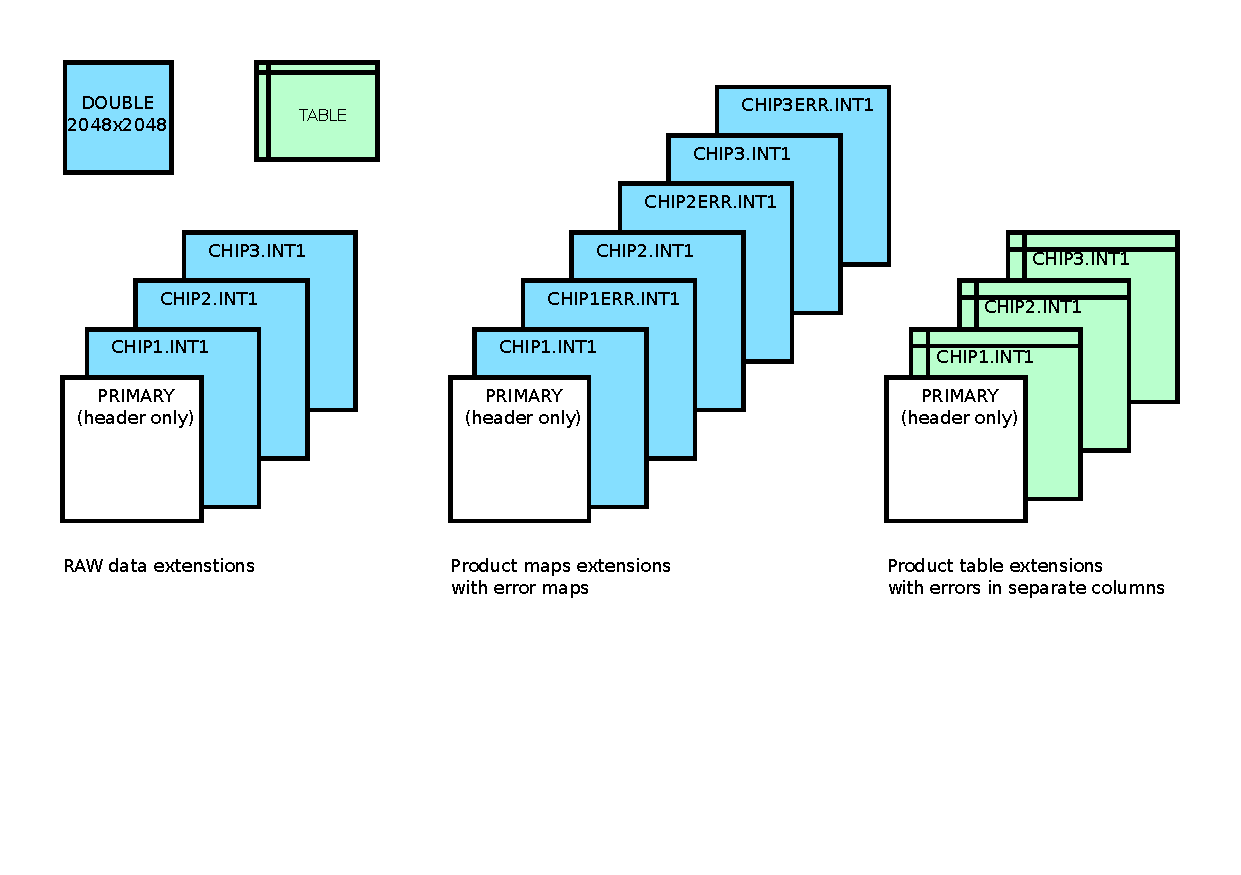
\includegraphics[width=0.99\linewidth]{fits_ext.pdf}
  \end{center}
  \caption{
    \label{fig:fits_ext}
    FITS extenstions in raw frames and data products.
    }
\end{figure}

Raw data comes as FITS files that contain no data, only headers in the
primary extension, and one image extension with the readout result from each
detector. The latter are named like \texttt{CHIPn.INT1} where \texttt{n} is
the detector number (1..3), in order from left to right with increasing
wavelength in each spectral order.

Data reduction products are either FITS tables or images. The separation
of data from the detectors is kept, and most recipes treat them independently.
For derived maps or images that have errors, three more extension are 
present, named like \texttt{CHIPnERR.INT1}.

Fig.~\ref{fig:fits_ext} illustrates this. The extensions are usually ordered, however we recommend to no rely on the index when opening files with custom
scripts or tools. Instead, the FITS extension \emph{name} should be used.

\subsubsection{The TraceWave-Table}
\label{sec:tracewave}

The most important FITS table within the \instrument\ DRS is the \emph{TraveWave}, abbreviated TW henceforth. It contains information about
how spectral orders are located in the detectors' pixel grid, how the
projection of the slit changes, and the wavelength solution.

Each row in the table corresponds to a single \emph{trace}. Each trace
belongs to a single spectral order; an order can have one or more traces,
numbered starting with 1 within each order.
The order number and trace number are two of the columns in the TW table, and together they uniquely identify a trace, i.e.~a table row.

Each trace stores three polynomials: one for the mid-line, upper and lower edge, respectively. Polynomials are stored as coefficients, lowest power
first, and evaluated for pixel columns starting with index 1.

Analogously, the wavelength solution is stored as polynomial coefficients that represent the translation from pixel to wavelength space.

meta-polynomials for slit curve.



\subsubsection{Pixels, Indices and Spectral Bins}
Pixel index starts at 1, not 0.

Also true when evaluating polynomials like race or wavecal.

Spectral bins correspond to detector columns at the mid-line of the extracted region (constant height).

Orders are indexed from 1..9, not always starting at 1, depending on cut-off orders. Index set by headers, conversion
to order number $m$ by XXX...

\subsection{The Pipeline Recipes}
\label{sec:recipes-quick}

\red{\textit{Overview and/or summary of available pipeline recipes, i.e. list
    of available pipelines and a brief (one-liner) description of its purpose.}}

The naming convention groups the recipes into
\begin{itemize}
    \item \textit{Calibration recipes}, named like \texttt{cr2res\_cal\_*}
    \item \textit{Observing recipes}, named like \texttt{cr2res\_obs\_*}
    \item \textit{Utility recipes}, named like \texttt{cr2res\_util\_*}
\end{itemize}


\begin{figure}[!tb]
  \begin{center}
    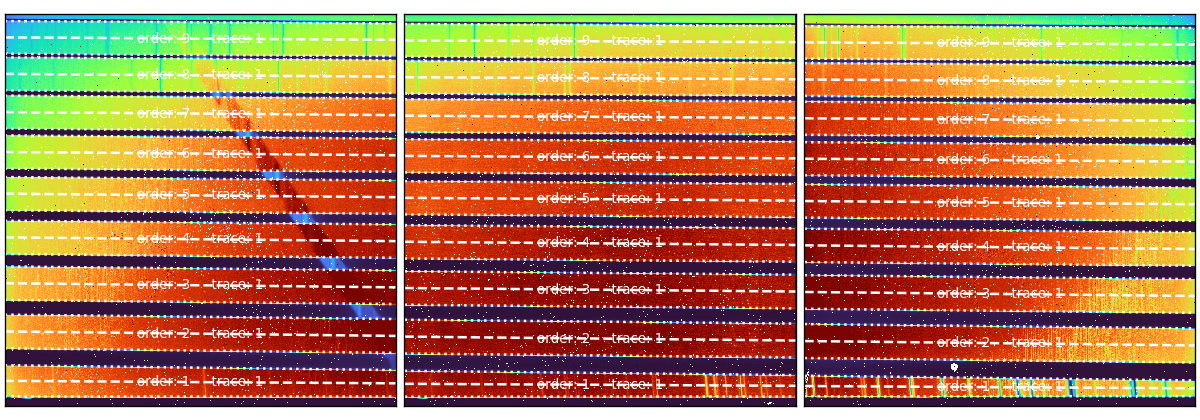
\includegraphics[width=0.99\linewidth]{J_2_3_03_cr2res_util_trace_out.png}
  \end{center}
  \caption{
    \label{fig:flat_trace}
    An example of a raw flat-field frame in J/2/3. Overplotted in white is 
    the result of the order tracing, the polynomial fit to the mid-line
    (dashed) and edges (dotted) for each detector-order.
    }
\end{figure}


%%%
%%%%%%%%%%%%%% SCIENCE ABOVE  %%%%% CALIBS BELOW
%%%%

\subsection{Reducing Calibrations}
\label{sec:calib:reduc}

The following instrument properties need to be characterized:
\begin{itemize}
    \item Detector: non-linearity
    \item Detector: dark current
    \item Detector: bad pixel map
    \item Flat-fielding\footnote{By \textit{flat-field} we always mean the
              normalized pixel-to-pixel variations
              in sensitivity, not the response at larger scales.}
    \item The location and shape of the spectral orders on each detector.
    \item The orientation (tilt) of the slit within each order.
    \item Wavelength calibration.
\end{itemize}

The \emph{detector non-linearity} is derived from a long series of flat-field
frames. These are not taken on a frequent basis and are valid for a long time.
Users will almost always be able to use the provided master calibration and not
need to run this step.

The \emph{master dark} is ideally derived from dark exposures with the
same DIT, and as high NDIT as possible. For short exposures the dark current
itself is negligible, but the detector readout-mode leaves a residual pattern
that scales non-trivially with DIT, so that scaling dark by unmatched exposure
time is not recommended.

Darks exposures are not really "dark", but contain come background thermal emission,
especially in the longer bands. Therefore, Darks are considered specific to
each instrument setting.

The \emph{master flat} is derived from a halogen lamp exposure; it is specific
to each spectrograph setting, for obvious reasons. By \emph{flat-field} the DRS
means the \emph{normalized flat-field}, that is the pixel-to-pixel sensitivity
variations, alone. The wavelength-dependency within each spectral order is
saved as the \emph{blaze} to a separate data product.

\emph{Bad pixel masks} can come from several steps
\begin{itemize}
    \item darks, rejecting outliers like hot and dark pixels.
    \item flats, rejecting pixels outside a range of sensitivity.
    \item detlin, rejecting pixels with deviating linearity behaviour.
    \item edge pixels. Each detector has 4 colunms and rows at the edges that
        are tnot sensitive to light.
    \item inter-order, masking the pixels that are not part of a spectral order.
\end{itemize}

Therefore, several recipes produce BPMs and there are recipes that can merge
and separate them.

Except for the detector linearity, calibrations are valid only for a
single setting (band \& echelle) and there are a number of \textit{fixed
standard settings} defined that cover the spectral range in all the bands,
including the gaps between detectors. While DRS should in principle be able to
handle non-standard settings just fine, this is not supported for the time
being.


\begin{figure}[!tb]
    \begin{center}
        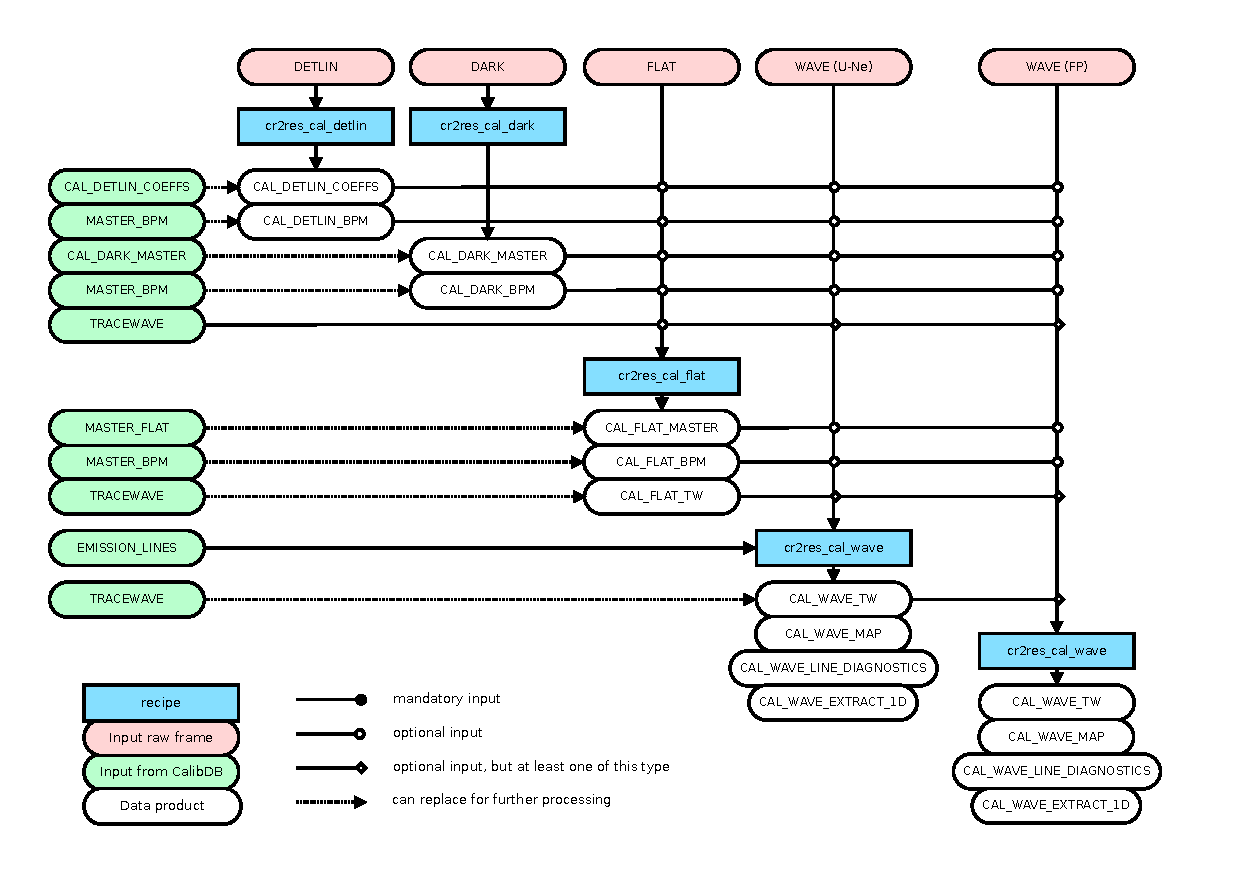
\includegraphics[width=0.99\linewidth]{calib_simple.pdf}
    \end{center}
    \caption{
        \label{fig:calibflow_simple}
        Flow diagram for calibration reduction with the \textit{calibration
        recipes}, assuming a populated CalibDB exists. Arrows and lines
        indicate the inputs to the recipes (blue), in the form of raw data
        (red), master calibrations from the CalibDB (green), or intermediate
        products from previous steps (white). Dotted lines indicate when a
        CalibDB or intermediate product can be chosen for later steps
        further to the right. All line connections are optional (open
        symbols), but generally recommended to be present. Also note that
        open diamonds mark Tracewave (TW) inputs, of which at least one
        needs to be present.
        \newline
        If a TW is provided to \texttt{cr2res\_cal\_flat}, it will use the
        information therein; otherwise it performs the tracing of the spectral
        orders to find their location. However, the slit tilt cannot be
        determined from flat-field frames which means that the extraction of the
        blaze function will be done assuming a vertical slit, yielding
        sub-optimal results. Therefore providing the TW from the CalibDB is
        recommended.
    }
\end{figure}


\begin{figure}[!tb]
    \begin{center}
        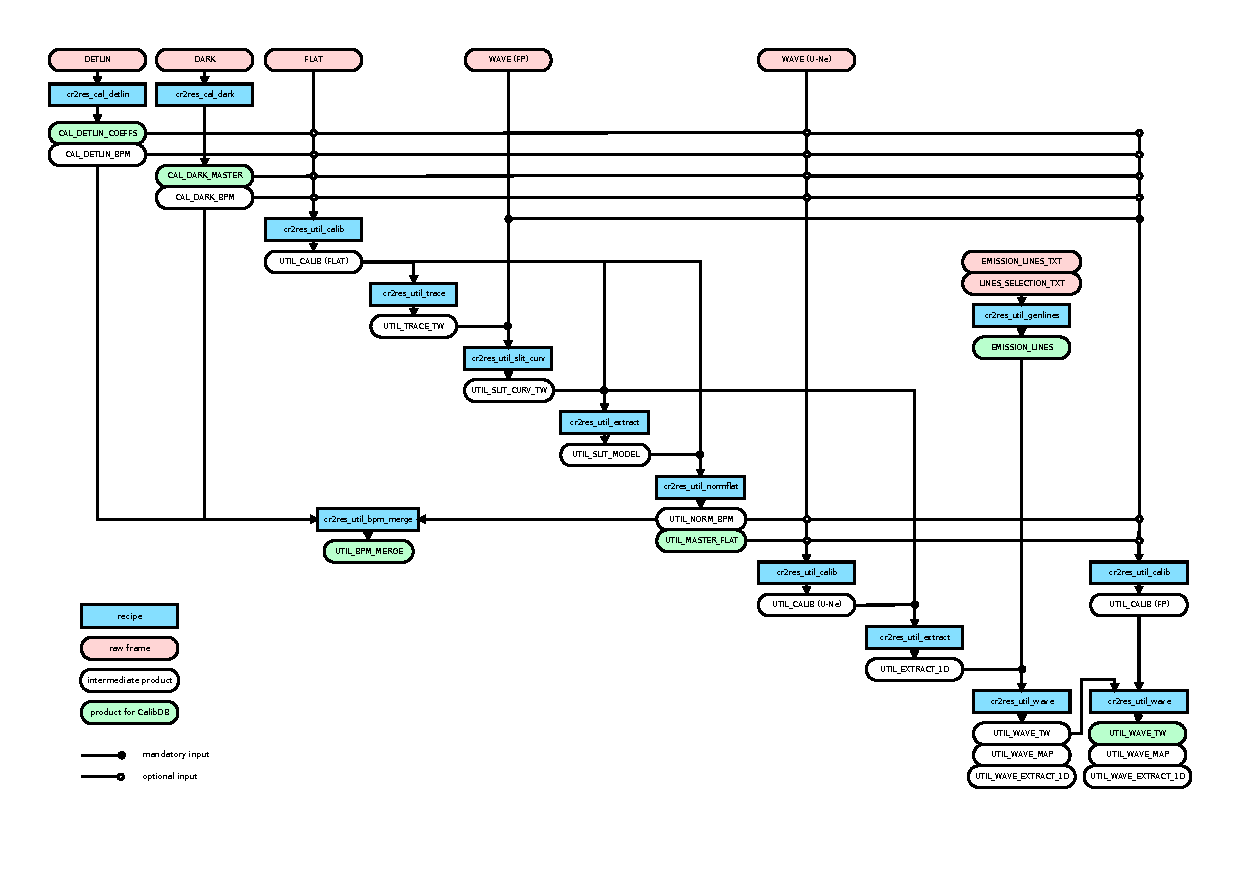
\includegraphics[width=0.99\linewidth]{calib_detailed.pdf}
    \end{center}
    \caption{
        \label{fig:calibflow_detailed}
        Flow diagram for calibration reduction with the \textit{utility
            recipes},
        without relying on any input from the CalibDB. In other words, this is
        how the products for the CalibDB (green) can be made from scratch.
        Steps
        are
        numbered but execution order can be changed whenever data flow allows.
        For
        notes on individual steps see main text.
    }
\end{figure}

Fig.~\ref{fig:calibflow_detailed} shows the calibration data flow cascade
step-by-step, using the \emph{util} recipes that only perform a single task
each:
\begin{enumerate}
    \item \texttt{cr2res\_util\_genlines} creates the catalogue files for each
          setting,
          based on the base catalogue and selection files that mark wavelength
          regions
          that are flagged as good for a certain setting.
    \item \texttt{cr2res\_cal\_detlin} takes flat-field exposures from
          different settings and with varying exposure times to measure the
          linearity
          behaviour of all pixels. Outliers get flagged as a bad-pixel-map
          (BPM).
    \item \texttt{cr2res\_cal\_dark} combines the input DARK frames into a
          master dark for
          each setting and combination of DIT and NDIT. Hot and dead pixels get
          saved as BPM.
    \item \texttt{cr2res\_util\_calib} combines the raw FLAT frames and applies
          the	       previous master calibs.
    \item \texttt{cr2res\_util\_trace} finds continuous regions on the
          detectors that
          have signal, and fits them with polynomials for the orders' mid-lines
          and edges.
          These polynomials we call a \emph{trace} and each order can have more
          than one,
          e.g. marking different heights along the slit.
    \item \texttt{cr2res\_util\_slit\_curv} uses the TraceWave-table (TW) from
          the previous
          step to measure the lines a FP-Etalon WAVE frame and determine how
          the
          slit tilt
          changes within each detector-order. The result is stored in an
          updated
          TW.
    \item \texttt{cr2res\_util\_extract} can now use this TW to extract the
          previously
          calibrated flat-field frame, resulting in the blaze spectrum and a
          model of
          the frame.
    \item This model contains all non-local features, meaning that
          \texttt{cr2res\_util\_normflat} can calculate the normalized
          flat-field
          by
          dividing the model by the the original frame. Outliers in sensitivity
          get
          flagged in another BPM.
    \item \texttt{cr2res\_util\_bpm\_merge} merges the BPMs from the different
          sources.
    \item \texttt{cr2res\_util\_calib} merges WAVE frames and applies the
          previous
          calibrations.
    \item \texttt{cr2res\_util\_extract} collapses the result from the last
          step into
          1D spectra.
    \item \texttt{cr2res\_util\_wave} uses these spectra and the catalogue of
          lines to
          derive a wavelength solution, i.e.~a polynomial that translates
          pixel-coordinates
          into wavelength (nm). Available methods include cross-correlation and
          line-fitting. This step can be repeated, for example to step-wise
          increase the
          polynomial degree.
    \item[13-15.] Analogous to steps 10-12 but for a FP-Etalon frame this time.
          The Etalon method of \texttt{cr2res\_util\_wave} will use the
          zero-point
          and dispersion from the incoming previous wavecal (in TW) and refine
          the
          higher degrees of the solution.
\end{enumerate}
\section{Data Reduction Cook-Book}
\label{sec:cookbook}

%\red{\textit{Cookbook-like description of pipeline recipes and their usage}}

\subsection{Getting Started with \esorex{}}
\label{sec:esorex-quick}

\textit{\esorex{}} is a command-line tool which can be used to execute the
recipes of all standard VLT/VLTI instrument pipelines. With \textit{\esorex{}}
in your path, the general structure of an \textit{\esorex{}} 
command line is

\begin{shell}[fontsize=\small]
%prompt esorex [esorex options] [recipe [recipe options] [sof [sof]...]]
\end{shell}

where options appearing before the recipe name are options for
\textit{\esorex{}} itself, and options given after the recipe name are options
which affect the recipe. 

All available \textit{\esorex{}} options can be listed with the command
\begin{shell}[fontsize=\small]
%prompt esorex --help
\end{shell}

and the full list of available parameters of a specific recipe can be obtained
with the command 

\begin{shell}[fontsize=\small]
%prompt esorex --help <recipe name>
\end{shell}
The output of this command shows as parameter values the current setting, \ie
all modifications from a configuration file or the command line are already
applied.

The listing of all recipes known to \textit{\esorex{}} can be obtained with the command
\begin{shell}[fontsize=\small]
%prompt esorex --recipes
\end{shell}

The last arguments of an \textit{\esorex{}} command are the so-called
\textit{set-of-frames}. A \textit{set-of-frames} is a simple text file which
contains a list of input data files for the recipe. Each input file is
followed by an unique identifier (frame classification or frame tag),
indicating the contents of this file. The input files can be given as 
absolute or relative path, and \textit{\esorex{}} allows the use of environment variables so
that a common directory prefix can be abreviated. Individual lines may be
commented out by putting the hash character (\texttt{\#}) in the first
column. An example of a \textit{set-of-frames} is shown in the following:

\begin{shell}[fontsize=\small]
%prompt cat darks.sof
/data/crires/CRIRES.2019-03-29T09:50:36.645.fits DARK
$RAW_DATA/CRIRES.2019-03-29T09:52:16.513.fits DARK
$RAW_DATA/CRIRES.2019-03-29T09:53:47.996.fits DARK
#$RAW_DATA/CRIRES.2019-03-29T09:55:04.515.fits DARK
#$RAW_DATA/dark5.fits DARK
\end{shell}

These \textit{set-of-frames} files will have to be created by the user using a
text editor, for instance.

Finally, if more than one \textit{set-of-frames} is given on the command-line
\textit{\esorex{}} concatenates them into a single \textit{set-of-frames}.


\subsection{Calibration, made easy}
\label{sec:simcalexpl}
This example follows the data flow described in \ref{sec:simplecalib}. It makes
use of a pre-existing TW-table, for example the one from the CalibDB, for order
traces and slit-tilt. All data needs to match in spectrograph setting.

\texttt{cr2res\_cal\_dark} only receives raw frames, so the SOF looks like the
one just above and gets processed like
\begin{shell}[fontsize=\small]
  %prompt esorex cr2res_cal_dark darks.sof
\end{shell}  
The outputs are master darks and BPM. The recipe parameters influence how
outliers are rejected and where to put the threshold for rejecting pixels as
bad. The default values should give good results.

Next are the FLATs.
\begin{shell}[fontsize=\small]
%prompt cat flats.sof
$RAW/flat1.fits         FLAT
$RAW/flat2.fits         FLAT
$RAW/flat3.fits         FLAT
$CALIB/dark_bpm.fits    CAL_DARK_BPM
$CALIB/dark_master.fits CAL_DARK_MASTER
$CALIB/tw.fits          UTIL_WAVE_TW
cr2res_detlin_coeffs.fits  CAL_DETLIN_COEFFS

%prompt esorex cr2res_cal_flat flats.sof
\end{shell}
The main data product is the normalized flat-field
(\verb!PRO.CATG=CAL_FLAT_MASTER!). Note that even though the recipe can perform
the order-tracting by itself, it is recommended to provide a TW as input;
especially in the bands YJHK, where the slit-tilt can be characterized. This way
absorption lines affect the flat-field less.


For wavelength-calibration, both the UNE and FPET frames should best be provided
at once:
\begin{shell}[fontsize=\small]
%prompt cat wave.sof
$RAW/une.fits           WAVE_UNE
$RAW/fpet.fits          WAVE_FPET
$CALIB/dark_bpm.fits    CAL_DARK_BPM
$CALIB/dark_2s_master.fits CAL_DARK_MASTER
$CALIB/tw.fits          UTIL_WAVE_TW
$CALIB/cr2res_detlin_coeffs.fits  CAL_DETLIN_COEFFS

%prompt esorex cr2res_cal_wave wave.sof
\end{shell}
This produces a new TW, with updated wavelength solutions and retaining information like the order traces from the input TW.

In this simplified reduction, we rely on a pre-existing TW for traces and slit-tilt, and pre-made non-linearity correction. This normally should not negatively impact the quality of the data products, especially when metrology is used to increase the repeatability of the instrument.

%%%%%%%%%%%%%%%%%%
%%%%%%%%%%%%%%%%%%
\subsection{Examples of science reductions}

\subsubsection{Nodding}
\label{sec:nodding}
An example SOF and esorex-call for \verb!cr2res_obs_nodding! were already shown
in Ch.~\ref{sec:sci-reduc} and there really is not much more to it. Note that
there is no master-dark provided, and indeed it is not recommended doing so,
because it likely worsens the results compared to relying on the subtraction of
A and B frames from each other for removing detector features and background.

An aspect to consider is how much of an observed nodding sequence is given to
the recipe at a time. It will combine all the A-frames and all B-frames (saved
as \verb!PRO.CATG=OBS_NODDING_COMBINED[AB]!), then do the pair-wise subtraction
and spectrum extraction, resulting in a single set of spectra (from all
detector-orders) for A, and one for B (\verb!OBS_NODDING_EXTRACT[AB]!).
Therefore, if time-evolution plays a role in the science, a set of data might
need to be split up and reduced individually. An equal number of frames for
positions A and B always needs to be supplied.

The recipe also produces spectra that are combined from A and B
(\verb!OBS_NODDING_EXTRACT_COMB!). This naturally involves resampling and
relying on the wavelength scale, because the tilted slit makes the spectral
binning different between the top and bottom halves of the slit. This is why the
spectra \emph{before} this combination are considered the primary data product.
The combined spectrum contains the summed ADUs from A and B.

The jitter around positions A and B does not need to be treated explicitly by
the DRS. Instead, it makes use of the fact that the extraction algorithm
(cf.~\ref{sec:extract}) can handle arbitrary slit-illumination functions, in
this case the combined frame simply looks like multiple "stars" along the slit.

A few parameters can be tweaked to potentially improve results. If there remain
detector features that correlate with the detector columns in the combined
frames, as has sometimes been found to be the case,
\verb!--subtract_nolight_rows! can be set to \verb!TRUE!. This makes use of the
bottom 40 rows of the detectors which are intentionally baffled to not receive
light. A vertical median over these rows is calculated, and the result subtracted
from the image row-by-row.

The oversampling of the slit-function can be changed via
\verb!--extract_oversample!. This affects linearly the calculation effort of the
extraction, which in turn is the bulk of the total recipe runtime, so that
increasing the oversampling from a factor of 5 to 10 means the reduction takes
twice as long. In general, values below 5 give suboptimal results and values
above 10 are appropriate when the slit-illumination changes sharply. See
Ch.~\ref{sec:extract} for more details.

In addition to the aforementioned data products, the recipe also saves two new
TW tables with \linebreak\verb!PRO.CATG=OBS_NODDING_TW[AB]!. These correspond to
the lower and upper halves of the slit, i.e. the A and B nodding positions, and
thus have their respective slit-fractions set to \verb![0.0, 0.25, 0.5]! and
\verb![0.0, 0.75, 1.0]!. They can come handy, for example, to re-run the
extraction of a \verb!OBS_NODDING_COMBINED[AB]! frame, using
\verb!cr2res_util_extract!; or to over-plot the traces on the combined frame to
check the alignment of the target.

\subsubsection{Extracting multiple sources in nodding}
\label{sec:slitfracbinary}
In the case when multiple targets are placed on the slit (e.g resolved binary
stars) in nodding observations, a few simple steps are needed to extract the spectrum 
of each target separately. In the remainder of this section, we assume the user 
wishes to extract the spectra of two stars on the slit. The procedure can be 
adapted to handle any number of extractions.
 
Run the \verb!cr2res_obs_nodding! recipe with the default slit height.
This step is detailed in Ch.~\ref{sec:nodding} and an example SOF file is
shown in Ch.~\ref{sec:sci-reduc}.
From this step, we can disregard the extracted spectrum (as the recipe extracts
a single spectrum for the entire slit). However, we will use the combined
pair-wise subtracted A and B frames (\verb!PRO.CATG=OBS_NODDING_COMBINED[AB]!)
 illustrated in Fig.~\ref{fig:binary-nodding}.

\begin{shell}[fontsize=\small]
    %prompt esorex cr2res_obs_nodding nodd.sof
\end{shell}

\begin{figure}[!h]
  \begin{center}
    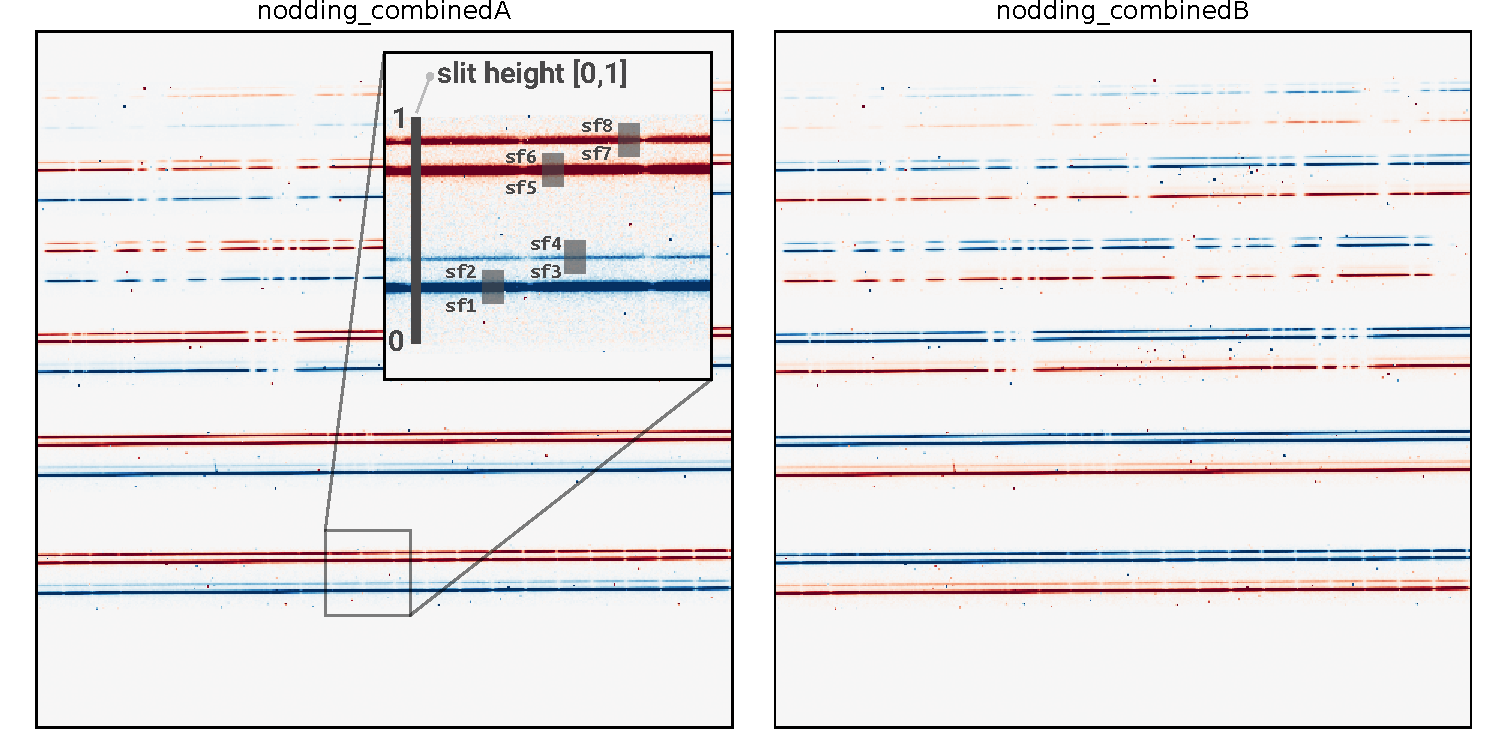
\includegraphics[width=1\textwidth]{figures/binary-nodding-combined}
  \end{center}
  \caption{
    \label{fig:binary-nodding}
    The two plots show the combinedA and combinedB frames
    on one detector. The inset on the left subplot zooms on a part of a
    spectral order, indicating the full slit height, 
    and illustrating slit fraction values to extract the spectra.}
\end{figure}

Extract the spectra of the two stars from the nodding position A -
hereafter named A1 and A2. This is done by running the \verb!cr2res_util_extract!
recipe on the combinedA frame twice, specifying slit fraction values adequate
for each of the two spectra, as illustrated in Fig.~\ref{fig:binary-nodding}.

Repeat the previous step on the combinedB frame to extract the spectra
B1 and B2, specifying adequate slit fractions.

\begin{shell}[fontsize=\small]
    %prompt mkdir A1 A2 B1 B1 # create directories to store spectra
    %prompt esorex --output-dir=A1 cr2res_util_extract --slit_frac=0.23,0.30 A.sof
    %prompt esorex --output-dir=A2 cr2res_util_extract --slit_frac=0.35,0.45 A.sof
    %prompt esorex --output-dir=B1 cr2res_util_extract --slit_frac=0.74,0.84 B.sof
    %prompt esorex --output-dir=B2 cr2res_util_extract --slit_frac=0.86,0.97 B.sof 
\end{shell}

The values of the slit-fraction listed here match the example from the figure;
they need to be adapted for each observation! The range of \verb![0.0 ... 1.0]!
corresponds to the [bottom ... top] edge 

The SOF files \verb!A.sof! and \verb!B.sof! contain only the TW file and
\begin{shell}[fontsize=\small]
    cr2res_obs_nodding_combinedA.fits OBS_NODDING_OTHER
\end{shell}
for \verb!A.sof!, and the equivalent combinedB frame for \verb!B.sof!.
No calibrations needed, because they are already applied to the combined frame.

If the user wants a single spectrum from nodding position A and for each of the
star, they still need to combine the A and B spectra -- essentially interpolating
one to the wavelength scales of the other.

\subsubsection{Staring}

\verb!cr2res_obs_staring! is very similar to \verb!cr2res_obs_nodding!, except
the nodding part. Thus, a master-dark should be supplied in the SOF, in addition
to the other files:
\begin{shell}[fontsize=\small]
%prompt cat stare.sof
$RAW/stare_exp1.fits        OBS_STARING_JITTER
$RAW/stare_exp2.fits        OBS_STARING_JITTER
$RAW/stare_exp3.fits        OBS_STARING_JITTER
$RAW/stare_exp4.fits        OBS_STARING_JITTER
$RAW/stare_exp5.fits        OBS_STARING_JITTER
$CALIB/K2192_masterflat.fits                  CAL_MASTER_FLAT
$CALIB/K2192_tw.fits                          UTIL_WAVE_TW
$CALIB/cr2res_cal_dark_K2192_bpm.fits         CAL_DARK_BPM
$CALIB/cr2res_cal_dark_K2192_30s_master.fits  CAL_DARK_MASTER
$CALIB/cr2res_detlin_coeffs.fits              CAL_DETLIN_COEFFS
\end{shell}  
Ideally, the DARK frames should match the DIT of the science frames.

If the target is always close to the center of the slit, one can decrease the extraction height for speedup.
\begin{shell}[fontsize=\small]
  %prompt esorex --extract_height=50 cr2res_obs_staring stare.sof
\end{shell}  

Analogous to the example of the binary star above, the option \verb!--slit_frac!
can be used to extract only a portion of the slit. This is useful to extract the
target and an empty portion of the slit, in order to perform sky-subtraction as
part of the analysis. Note that, due to the slit-tilt, the wavelength bins will
differ slightly between the spectra, so one needs to be resampled to the other.

\subsubsection{Generic Offset}

For data taken with the generic-offset-template, the DRS assumes that the
spatial resolution along the slit holds valuable information, and therefore does
not collapse the data into 1D-spectra. Instead, the recipe \verb!cr2res_obs_2d!
produces output tables with 2D spectra, where each in-order and not-bad pixel
has an entry with the following values and column names (prefixed with order and
trace number as for 1D spectra).

\begin{itemize}
    \item \verb!POSITIONX!, the original X-coordinate of the pixel
    \item \verb!POSITIONY!, same for Y
    \item \verb!SLIT_FRACTION!, from $[0..1]$, the spatial coordinate along the slit, i.e.~on sky.
    \item \verb!WL!, the wavelength
    \item \verb!SPEC!, the spectrum in ADU
    \item \verb!ERR!, the error spectrum.
\end{itemize}

Plotting the against wavelength and slit-fraction as X,Y-coordinates yields a
rectified 2D spectrum. Resampling to a regular grid is left to users.


The recipe interface of \verb!cr2res_obs_2d!, and thus the SOF files, follows
the same philosophy as the other \verb!cr2res_obs_*! recipes. The same processed
calibrations are listed together with the to-be-reduced raw frames.


The sky-pointings are subtracted from the object-pointings like this:

\begin{verbatim}
    if Number of SKY == Number of OBJ
         Loop on OBJ frames
             Subtract the corresponding SKY (same position in the list),
               applying the DIT correction ratio.
             Execute 2D-extraction
    else
         Average the SKY frames (if any)
         Loop in OBJ frames
             Subtract the Averaged Sky (if any) regardless of the DIT
             Execute 2D-extraction
\end{verbatim}         

\subsubsection{Polarimetry}

In polarimetry, the spectropolarimetry unit is inserted into the light path
ahead of the slit. It splits the incoming light beam into two parallel beams
of orthogonal polarization state, which then pass through a slit mask (also 
called deckers). There are two deckers: one lets the light through the first
and third quarter of the slit (each of them is 2.5" high), the other one
through the second and fourth quarter (cf.~RD01\cite{CIRESMAN}).
These two deckers are designed to cover two nodding positions, and the recipe
\verb!cr2res_obs_pol! is used in a completely analogous way to the nodding-recipe.

The SOF therefore looks just like the example from \ref{sec:sci-reduc}, except
that the raw frames are tagged \linebreak\verb!OBS_POLARIMETRY_OTHER! instead.
In addition, the recipe expects the number of raw frames to be a multiple of
$8$. This is because the observing template always takes $4$ exposures at each
nodding position, with alternating rotations of the internal optical elements;
and because the number of AB-cycles is expected to be $>0$, for background
subtraction.

As usual, the provided master calibrations are applied first. 
For the reduction of position A, the four frames from B are averaged and
subtracted, and vice versa. This works because the deckers block the light in
the respective opposite quarters of the slit.

Then the two beams are extracted from each frame, using order traces for each
decker hole. This means more extractions than for non-polarimetric observations
which is why this recipe takes significantly longer to run.

The individual extracted spectra are then combined with each other, following
the demodulation scheme described by \cite{1997MNRAS.291..658D}. The
demodulation scheme minimizes instrumental effects and produces the following
results, saved in a FITS table that is analogous to non-polarized spectra:

\begin{itemize}
    \item Intensity spectrum, i.e.~the sum of all the beams. Table columns named like \verb!i_INTENS! where \verb!i! is the order number.
    \item The Stokes parameter spectrum, i.e.~\textit{V}, \textit{Q} or \textit{U}, normalized by the intensity spectrum. These are stored in the columns \verb!i_STOKES!. Which of the Stokes parameters was observed in a dataset should be clear from your data organization, but can also be seen from the header \verb!INS.POL.TYPE!.
    \item The Null spectrum normalized by the intensity spectrum. This is a diagnostic spectrum from the demodulation that characterizes the level of spurious polarization. In the ideal case, there should be no polarization signatures present in the Null spectrum. \verb!i_NULL!.
    \item Error spectra for each of the above, in columns named like these, plus the suffix \verb!_ERR!.
    \item The array of wavelengths for each of the spectral bins.
\end{itemize}

By default, \verb!cr2res_obs_pol! does not produce intermediate outputs like the
calibrated raw frames and the decker-traces for extraction. The recipe parameter
\verb!--save_group=1! can be used to save these for a single group of $8$ raw
files, the first group in this case. Using this option results in $40$
additional files that hold the calibrated and nodding-sutracted frames, the TWs,
and the extracted spectra before demodulation.

\subsubsection{Spectro-Astrometry}

Spectro-astrometry uses the instrument derotator to take spectra with different
position angles of the slit on the sky.

The recipe \verb!cr2res_obs_nodding! can get raw input tagged like
\verb!OBS_ASTROMETRY_OTHER! or \linebreak\verb!OBS_ASTROMETRY_JITTER!. Given a sequence of
these, it will separate them by position angle and reduce the set for each angle
separately, just like plain nodding observations, with the same outputs. Any
further steps are considered out of scope for the DRS and left to users.

\subsection{Optional Steps}

\subsubsection{Throughput from standard stars}
\label{sec:throughput}
The pipeline comes with a fixed list of spectrophotometric standard stars. When \texttt{cr2res\_obs\_nodding} checks the
on-sky coordinates of the currently reduced target, and if they match one of those stars, it compares the reduced spectrum to the 
reference. The resulting throughput gets saved into a separate
data product (PRO.CATG=OBS\_NODDING\_THROUGHPUT).

Note however, that absolute flux calibration is generally not 
possible with \instrument\ because of varying slit-losses.


\subsubsection{Refining the BPM}
\label{sec:bpmrefine}
Using only the BPM that comes from \texttt{cr2res\_cal\_dark} usually gives
satisfactory results. However, pixels can be marked as bad also by being
outliers in their non-linearity behavior, or in their overall sensitivity, i.e.
in the normalized flat-field. The respective recipes each produce a BPM, and
have parameters for the thresholds.

The recipe \texttt{cr2res\_util\_bpm\_merge} allows you to merge these BPMs into
a combined BPM; \linebreak\texttt{cr2res\_util\_bpm\_split} does the inverse,
that is splitting a BPM into its original components. This is possible because
these recipes keep track of why a pixel was marked as bad. When a BPM is then
used in subsequent reduction steps, any kind of bad pixel gets masked and does
not contribute to the result.

Note that BPMs are not checked to match in spectrograph setting, so that it is
possible to use a BPM from a one setting with data from another. The same is
true for DIT.

Experience has shown that the pair-wise subtraction via nodding makes many
pixels usable that were flagged as bad pixels from the DARK frames. It can
therefore make sense, especially for low S/N spectra, to use the BPM from from
\texttt{cr2res\_cal\_flat} instead (\verb!PRO.CATG=CAL_FLAT_BPM!). To do this,
one needs to
\begin{itemize}
    \item set the \verb!--bpm_kappa! for \texttt{cr2res\_cal\_dark} to a large value (e.g. 1000) to get a master dark without pixels marked as bad. This is because otherwise the flat-field would inherit the BPM from the master dark.
    \item adjust the parameters \verb!--bpm_low! and \verb!--bpm_high! for \texttt{cr2res\_cal\_flat} to appropriate relative sensitivity thresholds.
    \item use the \verb!CAL_FLAT_BPM! in subsequent reduction steps.
\end{itemize}

\subsubsection{Splicing and Continuum Normalization}

Give extracted spectra, blaze functions and TWs from several settings to
\texttt{cr2res\_util\_splice} and it will divide by the blaze, and resample the
overlap regions between all spectra from individual detector-orders onto a
common wavelength scale, in order to then combine them with a weighted average.
The result is a single spectrum, continuous over the regions covered by the
inputs.

\begin{figure}[!h]
  \begin{center}
    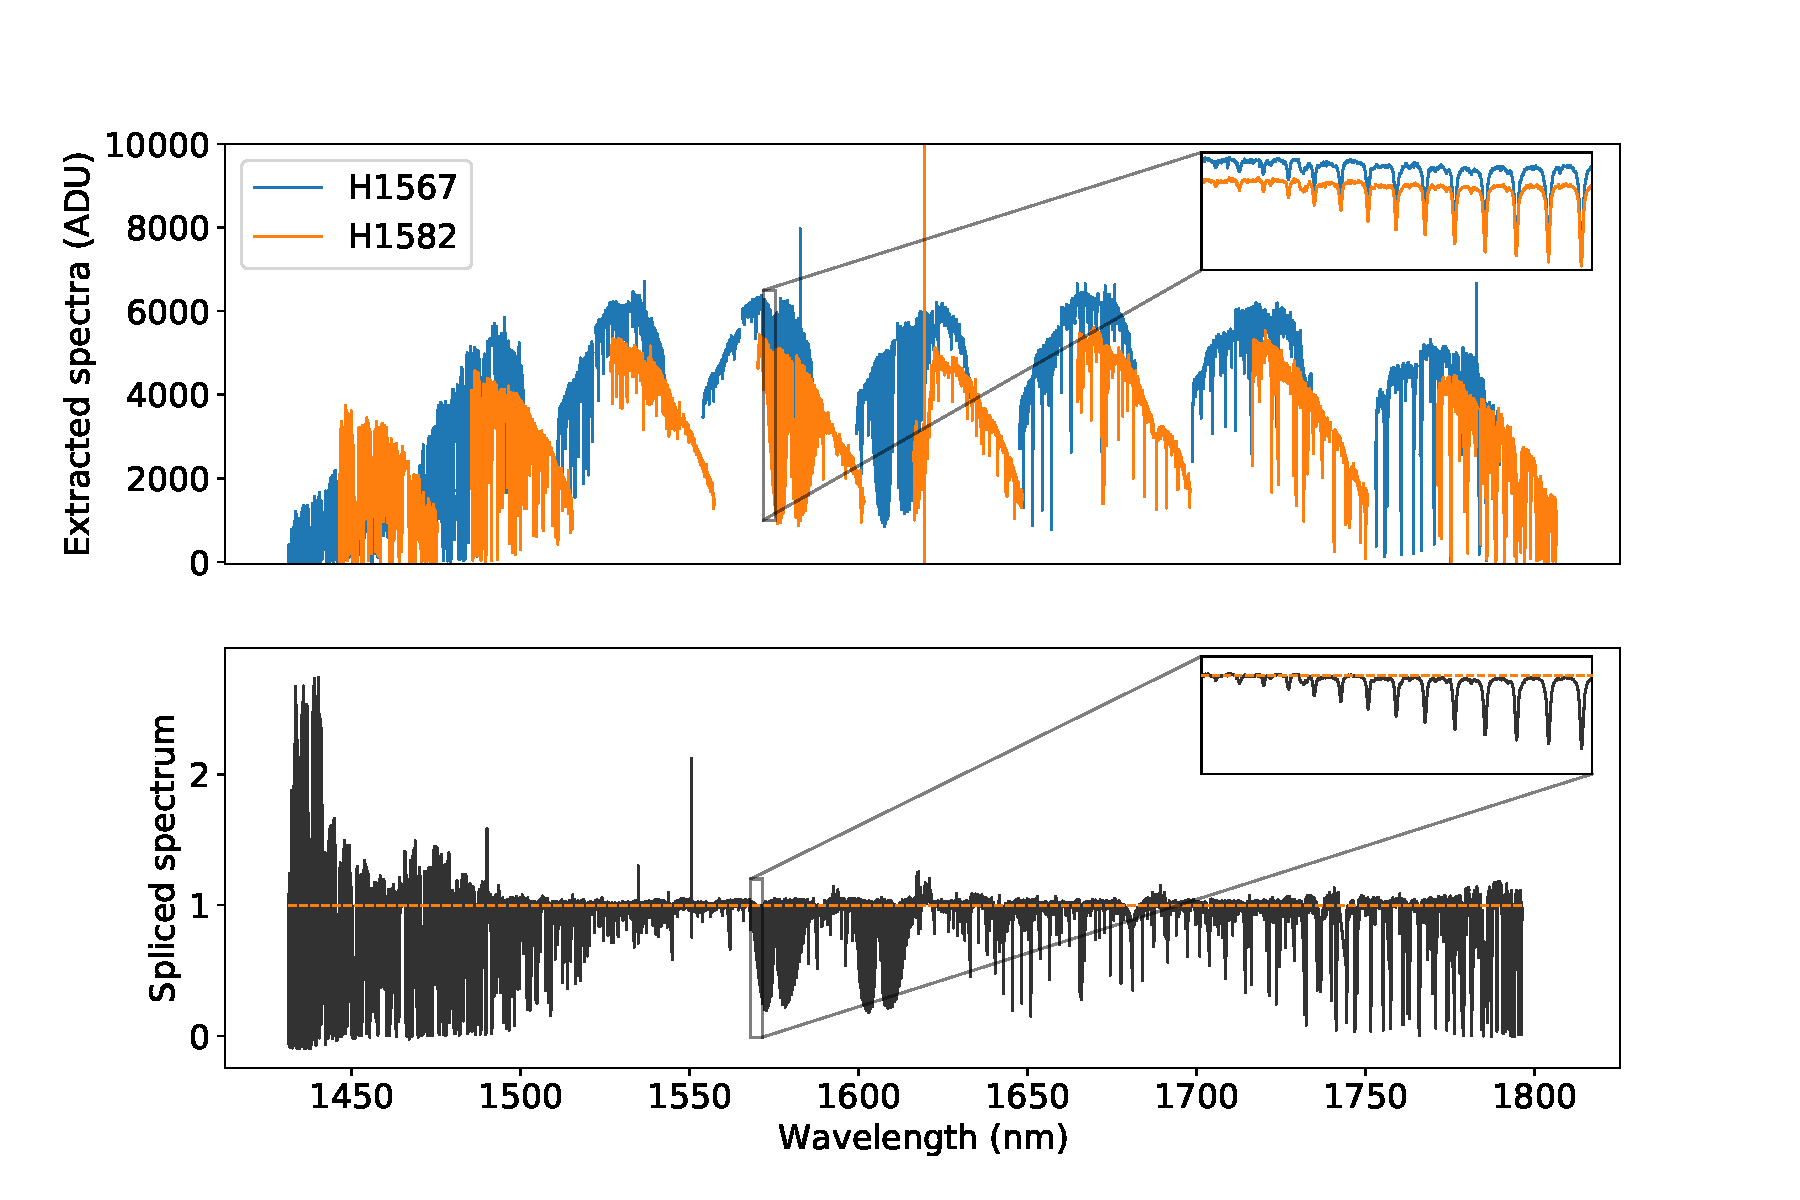
\includegraphics[width=1\textwidth]{figures/util_splice}
  \end{center}
  \caption{
    \label{fig:util_splice}
    The top subplot shows extracted spectra in two overlapping
    wavelength settings: H1567 and H1582 with an inset zoom to a narrow
    wavelength region. The bottom subplot shows the output of the splicing
    recipe. Notice that the normalization is far from perfect.}
\end{figure}

Please note that this recipe has not been tested extensively to produce reliable
results in all cases. For now its data products should therefore be considered
experimental and quality not ensured to be "science-ready". Fig.~\ref{fig:util_splice}
shows a typical example of what can be achieved with this recipe. An example SOF
file is printed below.

\begin{shell}[fontsize=\small]
%prompt cat splice.sof
H1567-cr2res_obs_nodding_extracted_combined.fits UTIL_EXTRACT_1D
H1582-cr2res_obs_nodding_extracted_combined.fits UTIL_EXTRACT_1D
$CALIB/H1567_tw.fits UTIL_WAVE_TW
$CALIB/H1582_tw.fits UTIL_WAVE_TW
$CALIB/H1567/05_cr2res_util_extract_out/
  cr2res_util_calib_calibrated_collapsed_extr1D.fits CAL_FLAT_EXTRACT_1D
$CALIB/H1582/05_cr2res_util_extract_out/
  cr2res_util_calib_calibrated_collapsed_extr1D.fits CAL_FLAT_EXTRACT_1D
\end{shell}

It should also be noted that it is probably a good idea to manually mask some
regions, like the ones affected by the ghosts, before splicing, since otherwise
this wavelength region would be degraded in the output, even if it was
unaffected in data from a different setting. 

\subsubsection{Blaze correction}

Most of the recipes performing a 1D extraction (cr2res\_obs\_staring,
cr2res\_obs\_nodding, cr2res\_obs\_pol) accept as optional input the 
blaze function computed by the cr2res\_cal\_flat recipe
(PRO CATG = CAL\_FLAT\_EXTRACT\_1D).
If the file is provided, the extracted spectrum is divided by the
normalised blaze function. The normalisation factor is the 95th
percentile of the blaze.

\subsection{Calibration, from scratch}
\label{sec:calibscratch}
Following the steps outlined in Ch.~\ref{sec:stepcalib} and accompanying text,
we can reduce the calibrations without relying on pre-existing reduction
products like the TW. This is also the way the static calibrations are
assembled. The following gives example SOFs and recipe calls to reduce a single
setting.

First the SOFs:
\begin{shell}[fontsize=\footnotesize]
%prompt cat 01_cr2res_cal_dark.sof
CRIRE.2021-09-16T20:58:23.580.fits      DARK     
CRIRE.2021-09-16T20:58:40.524.fits      DARK     
CRIRE.2021-09-16T20:58:57.146.fits      DARK     
CRIRE.2021-09-16T20:59:13.835.fits      DARK     
CRIRE.2021-09-16T20:59:30.110.fits      DARK     
CRIRE.2021-09-16T20:59:46.468.fits      DARK     
CRIRE.2021-09-16T21:00:08.583.fits      DARK     
CRIRE.2021-09-16T21:02:14.863.fits      DARK     
CRIRE.2021-09-16T21:04:21.006.fits      DARK     
CRIRE.2021-09-16T21:06:27.987.fits      DARK     
CRIRE.2021-09-16T21:06:54.976.fits      DARK     
CRIRE.2021-09-16T21:07:21.609.fits      DARK     
CRIRE.2021-09-16T21:07:48.034.fits      DARK     
CRIRE.2021-09-16T21:07:57.532.fits      DARK     
CRIRE.2021-09-16T21:08:06.919.fits      DARK     

%prompt cat 02_cr2res_util_calib.sof
../cr2res_cal_detlin_coeffs.fits CAL_DETLIN_COEFFS
CRIRE.2021-09-16T20:49:23.778.fits      FLAT     
01_cr2res_cal_dark_out/cr2res_cal_dark_Y1028_3_bpm.fits CAL_DARK_BPM
01_cr2res_cal_dark_out/cr2res_cal_dark_Y1028_3_master.fits CAL_DARK_MASTER

%prompt cat 03_cr2res_util_trace.sof
02_cr2res_util_calib_out/cr2res_util_calib_calibrated_collapsed.fits    UTIL_CALIB

%prompt cat 04_cr2res_util_slit_curv.sof
CRIRE.2021-09-16T20:54:28.992.fits      WAVE_FPET
03_cr2res_util_trace_out/cr2res_util_calib_calibrated_collapsed_tw.fits  CAL_FLAT_TW

%prompt cat 05_cr2res_util_extract.sof
02_cr2res_util_calib_out/cr2res_util_calib_calibrated_collapsed.fits UTIL_CALIB
04_cr2res_util_slit_curv_out/cr2res_util_calib_calibrated_collapsed_tw_tw.fits UTIL_SLIT_CURV_TW

%prompt cat 06_cr2res_util_normflat.sof
02_cr2res_util_calib_out/cr2res_util_calib_calibrated_collapsed.fits UTIL_CALIB
05_cr2res_util_extract_out/cr2res_util_calib_calibrated_collapsed_extrModel.fits UTIL_SLIT_MODEL

%prompt cat 07_cr2res_util_calib.sof
../cr2res_cal_detlin_coeffs.fits CAL_DETLIN_COEFFS
CRIRE.2021-09-16T20:50:11.966.fits      WAVE_UNE 
01_cr2res_cal_dark_out/cr2res_cal_dark_Y1028_20_bpm.fits CAL_DARK_BPM
01_cr2res_cal_dark_out/cr2res_cal_dark_Y1028_20_master.fits CAL_DARK_MASTER
06_cr2res_util_normflat_out/cr2res_util_normflat_Open_master_flat.fits CAL_FLAT_MASTER

%prompt cat 08_cr2res_util_extract.sof
07_cr2res_util_calib_out/cr2res_util_calib_calibrated_collapsed.fits UTIL_CALIB
04_cr2res_util_slit_curv_out/cr2res_util_calib_calibrated_collapsed_tw_tw.fits UTIL_SLIT_CURV_TW

%prompt cat 09_cr2res_util_genlines.sof
../lines_u_sarmiento.txt EMISSION_LINES_TXT
une_sel.dat LINES_SELECTION_TXT

%prompt # there is no step 10
%prompt cat 11_cr2res_util_wave.sof
08_cr2res_util_extract_out/cr2res_util_calib_calibrated_collapsed_extr1D.fits UTIL_EXTRACT_1D
04_cr2res_util_slit_curv_out/cr2res_util_calib_calibrated_collapsed_tw_tw.fits UTIL_SLIT_CURV_TW
09_cr2res_util_genlines_out/lines_u_sarmiento_une_sel.fits EMISSION_LINES

%prompt cat 12_cr2res_util_wave.sof
08_cr2res_util_extract_out/cr2res_util_calib_calibrated_collapsed_extr1D.fits UTIL_EXTRACT_1D
11_cr2res_util_wave_out/cr2res_util_calib_calibrated_collapsed_extr1D_tw.fits UTIL_SLIT_CURV_TW
09_cr2res_util_genlines_out/lines_u_sarmiento_une_sel.fits EMISSION_LINES

%prompt cat 13_cr2res_util_calib.sof
../cr2res_cal_detlin_coeffs.fits CAL_DETLIN_COEFFS
CRIRE.2021-09-16T20:54:28.992.fits      WAVE_FPET
01_cr2res_cal_dark_out/cr2res_cal_dark_Y1028_120_bpm.fits CAL_DARK_BPM
01_cr2res_cal_dark_out/cr2res_cal_dark_Y1028_120_master.fits CAL_DARK_MASTER
06_cr2res_util_normflat_out/cr2res_util_normflat_Open_master_flat.fits CAL_FLAT_MASTER

%prompt cat 14_cr2res_util_extract.sof
13_cr2res_util_calib_out/cr2res_util_calib_calibrated_collapsed.fits UTIL_CALIB
11_cr2res_util_wave_out/cr2res_util_calib_calibrated_collapsed_extr1D_tw.fits UTIL_SLIT_CURV_TW

%prompt cat 15_cr2res_util_wave.sof
14_cr2res_util_extract_out/cr2res_util_calib_calibrated_collapsed_extr1D.fits UTIL_EXTRACT_1D
11_cr2res_util_wave_out/cr2res_util_calib_calibrated_collapsed_extr1D_tw.fits UTIL_WAVE_TW
\end{shell}

The commands to execute the steps are:
\begin{shell}[fontsize=\footnotesize]
esorex --log-file=01_cr2res_cal_dark.log --output-dir=01_cr2res_cal_dark_out cr2res_cal_dark 
  01_cr2res_cal_dark.sof
esorex --log-file=02_cr2res_util_calib.log --output-dir=02_cr2res_util_calib_out 
  cr2res_util_calib --collapse="MEAN" 02_cr2res_util_calib.sof
esorex --log-file=03_cr2res_util_trace.log --output-dir=03_cr2res_util_trace_out    
  cr2res_util_trace 03_cr2res_util_trace.sof
esorex --log-file=04_cr2res_util_slit_curv.log --output-dir=04_cr2res_util_slit_curv_out
  cr2res_util_slit_curv 04_cr2res_util_slit_curv.sof
esorex --log-file=05_cr2res_util_extract.log --output-dir=05_cr2res_util_extract_out
  cr2res_util_extract --smooth_slit=3 -smooth_spec=2 
  05_cr2res_util_extract.sof
esorex --log-file=06_cr2res_util_normflat.log --output-dir=06_cr2res_util_normflat_out 
  cr2res_util_normflat 06_cr2res_util_normflat.sof
esorex --log-file=07_cr2res_util_calib.log --output-dir=07_cr2res_util_calib_out 
  cr2res_util_calib --collapse="MEAN" --subtract_nolight_rows=TRUE 07_cr2res_util_calib.sof
esorex --log-file=08_cr2res_util_extract.log --output-dir=08_cr2res_util_extract_out  
  cr2res_util_extract --smooth_slit=30 --swath\_width=2048  08_cr2res_util_extract.sof
esorex --log-file=09_cr2res_util_genlines.log  --output-dir=09_cr2res_util_genlines_out  
  cr2res_util_genlines 09_cr2res_util_genlines.sof
esorex --log-file=11_cr2res_util_wave.log --output-dir=11_cr2res_util_wave_out 
  cr2res_util_wave --wl_method=XCORR --wl_degree=0 --keep --wl_err=0.1 --fallback 
11_cr2res_util_wave.sof
esorex --log-file=12_cr2res_util_wave.log --output-dir=12_cr2res_util_wave_out 
  cr2res_util_wave --wl_method=XCORR --wl_degree=2 --wl_err=0.03 --fallback 
  12_cr2res_util_wave.sof
esorex --log-file=13_cr2res_util_calib.log --output-dir=13_cr2res_util_calib_out 
  cr2res_util_calib --collapse="MEAN" 13_cr2res_util_calib.sof
esorex --log-file=14_cr2res_util_extract.log --output-dir=14_cr2res_util_extract_out 
  cr2res_util_extract --smooth_slit=3 14_cr2res_util_extract.sof
esorex --log-file=15_cr2res_util_wave.log --output-dir=15_cr2res_util_wave_out 
  cr2res_util_wave --wl_method=ETALON --wl_degree=4 --fallback 15_cr2res_util_wave.sof
\end{shell}


A few notes on the recipe parameters used:
\begin{enumerate}
  \item[2.] Remember, without \verb!--collapse! the recipe would loop over the
  flat-field frames, dark-subtracting each, instead of doing so on the combined
  frame.
  \item[5.] Extracting the flat-field frames, we know the slit is evenly
  illuminated, so we can apply some extra smoothing along the slit. The slight
  smoothing (regularization, actually) of the blaze spectrum is necessary
  because there are column-by-column variations in the detectors that would
  otherwise become part of the blaze, not part of the normalized flat-field, as
  intended.
  \item[7.] For short exposures the detector background-level can vary
  significantly, so we use \linebreak \verb! --subtract_nolight_rows! to
  somewhat improve on suboptimal dark-subtraction.
  \item[9.] The first pass of cross-correlation with a sufficiently large
  search-radius (\verb!--wl_err!). \verb!--wl_degree=0! means that only a shift
  in the zero-point is allowed, which means that we have to \verb!--keep! the
  higher degrees of the input solution polynomial.
  \item[11.] The UNE frames have very little signal in some detector orders, we
  therefore increase the smoothing along the slit and extract the full detector
  width in one swath, in order to increase the reliability.
  \item[12.] It is possible to run second pass on the UNE wavecal with decreased
  search radius and increased polynomial degree. This is however \emph{not}
  recommended any longer, since it is enough to get the zero-point from the UNE
  and leave the higher degrees to be determined from the FPET.
  \item[15.] The numerous and regular lines of the FPET allow a polynomial with
  even higher degree.
  \item[9,11,15.] Without \verb!--fallback! the output would, in case of an
  error in a detector-order, not contain a solution for this order, thus
  precluding it from subsequent steps. With this option, the input solution gets
  propagated into the output, in case calibration fails.
\end{enumerate}

\section{Algorithms}
\label{sec:algorithms}

% \red{\textit{The first part contains the detailed discussion and the
%     mathematical description of the used algorithms. The second part contains
%     the recipe algorithm, i.e. a high-level description of the recipe
%     flow-chart and how it changes for different parameter settings.}}

\subsection{General Algorithms}
\label{sec:algorithms-general}

\subsection{Optimal Extraction}
\label{sec:extract}
\begin{figure}[ht]
    \begin{center}
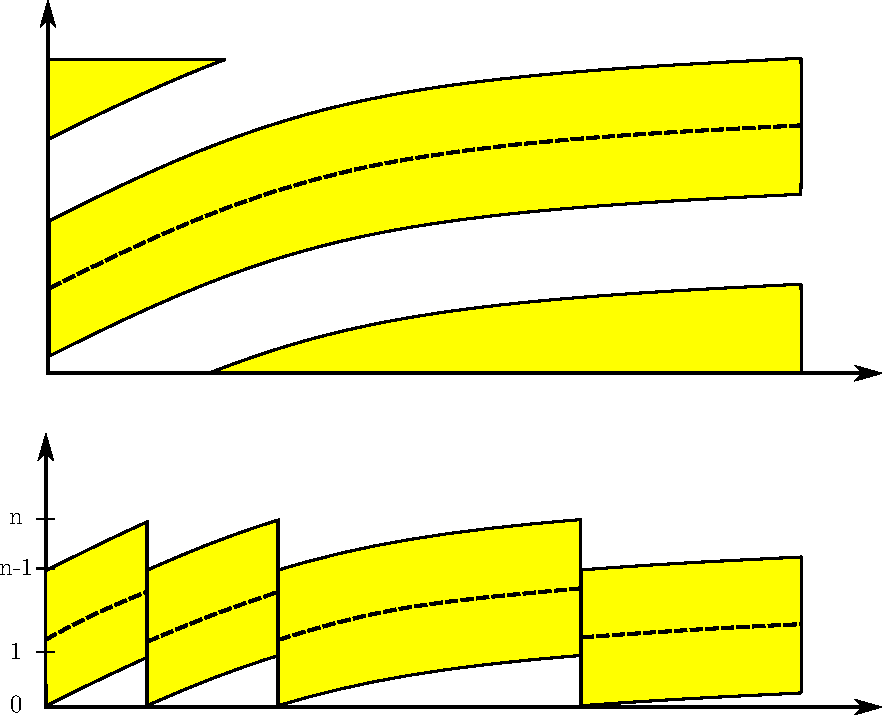
\includegraphics[width=0.45\linewidth]{rectification.pdf}
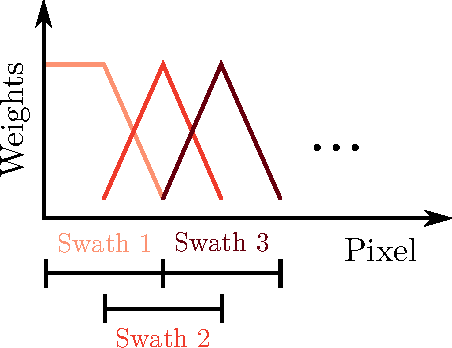
\includegraphics[width=0.45\linewidth]{swath_weights.pdf}
\end{center}
\caption{\it Left: Illustration of swath rectification. Right: The weights for combining the spectra from overlapping swaths.}
\label{fig:swaths}
\end{figure}

\begin{figure}[ht]
    \begin{center}
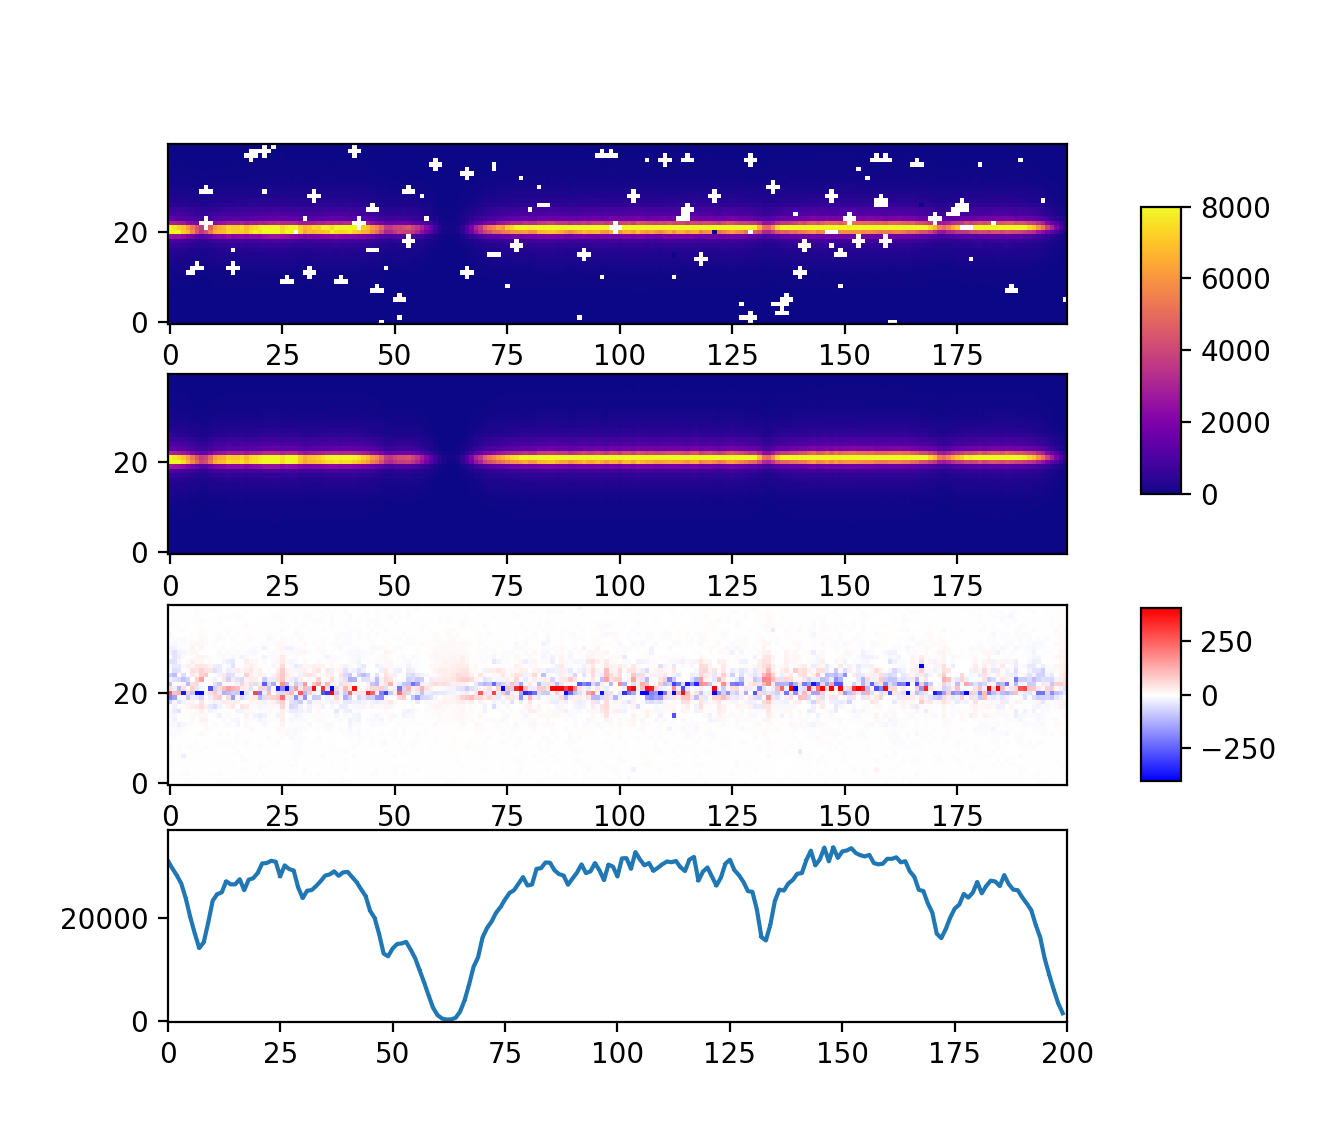
\includegraphics[width=0.85\linewidth]{extr_model.png}
\end{center}
\caption{An example of the optimal extraction. \emph{Top:} The flat-fielded,
combined, and pair-wise subtracted frame, with the BPM applied and zoomed-in to
part of a single spectral order. \emph{Panel 2:} The model of the same region,
reconstructed from the extracted spectrum and slit-function. \emph{Panel 3:} The
difference between the two above, showing the residuals. \emph{Bottom:} The extracted
spectrum itself, on the same x-axis as the panels above.}
\label{fig:extrmodel}
\end{figure}

The optimal extraction along the tilted and curved slit is a centerpiece of the
\instrument\ DRS and several recipes make use of it. Full details and
mathematical description can be found in \cite{2021A&A...646A..32P}. Here, we
simply summarize the most important practical implications from a user
perspective.

To extract a spectral order from a calibrated 2D frame into a 1D spectrum, using
a \emph{trace} from the TW table, the following steps are carried out:
\begin{itemize}
    \item Calculate the extraction height from the edge-polynomials, if not
    explicitly given via \texttt{-{}-extract\_height}.
    \item Cut out a rectangular region around the mid-line, called a
    \emph{swath} from the frame, using the height and the value of
    \texttt{-{}-extract\_swath\_width}.
    \item Rectify the swath by shifting columns by integer values such that the
    mid-line only retains values between $0\ldots 1$, like illustrated in
    \figref{fig:swaths} (left).
    \item Iteratively approximate the swath surface by two vectors: the spectrum
    along the mid-line and the slit-function along the slit projection, taking
    its changeing tilt into accont. The slit function is oversampled by a factor
    \verb!--extract_oversample!.
    \item Step by a half swath-width to the next one, and repeat. This way
    swaths overlap fully and the order effectively gets extracted twice.
    \item Once all swaths are extracted, the spectra from each are merged into
    one, with linearly in-/decreasing weights, as in \figref{fig:swaths}
    (right).
    \item The spectrum and slit-functions are saved, and used to reconstruct a
    2D model of the frame, saved separately.
    \item The errors are estimated from the residual between data and model.
\end{itemize}

A major advantage of this extraction algorithm is that it makes not assumption
about the slit-function, except that it does not change within a swath.

In addition, the model by design cannot approximate features that are not
present in all pixels that contribute to a certain bin in the spectrum or the
slit-function. This makes spectra robust towards e.g.~cosmic rays.

Fig.~\ref{fig:varyovers} shows the effect of the \textbf{slit-function
oversampling}, via  the parameter \verb!--extract_oversample!. As mentioned
before, this factor linearly affects the computation time. The amount of
oversampling necessary depends on how quickly the mid-line of a spectral order
changes with respect to detector rows, and how sharply the slit-function
changes. The default value of $5$ is enough in many situations, but clearly
leaves artifacts in the example shown, which was chosen to be close to
worst-case, requiring an oversampling $>12$ for optimal results.

\putgraph{.8\linewidth}{varyoversample.pdf}{varyovers}{Example spectrum,
 extracted with varying oversampling, and vertically offset for plotting.
 In this case, oversampling of 12 is needed to no longer see "spiky" artifacts.}

\subsection{Errors and Signal-to-Noise}
\label{sec:errors}


The normalization of the output-spectra is like that of a sum of pixel values,
collapsed along the slit, i.e. summed-up ADU. Errors are absolute.

If \verb!NDIT >1!, then a factor of $\sqrt{NDIT}$ needs to be taken into account,
because the sub-exposured were averaged in the detector software, not affecting
the ADU level.

\subsection{Recipes Algorithms} 
\label{sec:algorithms-recipes}


%\subsection{Nodding}
%\label{sec:nodd}
%Nodding sequence \texttt{SEQ.NABCYCLES} \texttt{SEQ.NODPOS}
%first combined, then calibs applied, then subtracted, then extraction

\subsubsection{Order Tracing}
\label{sec:ordertrace}

As written above, by a \emph{trace}, we mean a polynomial, in pixel-coordinates of a single detector, that follows the mid-line of a spectral order. And two more polynomials for the upper and lower edges of the slit projection, as shown in Fig.~\ref{fig:flat_trace}.

The way this is derived is by first determining which pixels in a FLAT frame contain signal, and which don't. To that end the image is smoothed first horizontally, then vertically, and then compared to the unsmoothed frame via thresholding.

After that it is determined which spectral order the pixels belong to. For this purpose, the mean Y-coordinate for each order is present in the raw file headers.

Lastly, the pixels from the same order are fitted with a polynomial.

%smooth in x. smooth strongly in y and compare to unsmoothed, threshold. unify
%clusters. label them. threshold minimum number od pix in cluster. fit
%%polynomial to all pix. fit edges.

\subsubsection{Measuring the slit-tilt}
\label{sec:tilt}

The recipe \verb!cr2res_util_slit_curv! takes as input a TW, for the order traces, and an FPET frame. The algorithm finds the etalon peaks, which give good coverage in each spectral order.

More detail will be provided in a future iteration of this document.

\subsubsection{Wavelength calibration}

There are several ways to calibrate the wavelength scale, and each corresponds
to one of the values that the parameter \texttt{-{}-wl\_method} of
\texttt{cr2res\_util\_wave} can take.

With \texttt{-{}-wl\_method=XCORR} the provided catalog of lines gets made into
a synthetic spectrum that is cross-correlated with the extracted lamp spectrum.
Each detector-order is calibrated separately.

The recipe \texttt{cr2res\_cal\_wave} combines two methods into one recipe, one
for the UNE lamp frames, and the one for the FPET. The result from the former
gets passed on to the latter, if both lamp inputs are present. If not, then only
the appropriate method is applied.
\section{Known Issues}
\label{sec:knownissues}

\subsection{Superresolution}
In good seeing conditions the AO system can produce a PSF that is sharp enough
to not evenly fill the slit width of the spectrograph. While this produces spectra with a resolution higher than specified, it can also cause an offset in the wavelength scale, because how the AO places the PSF center is not reproducible enough. Wavelength shifts between reduced spectra from the nodding positions A and B of around $1 pix$ have been encountered.

This is not something that the DRS can correct for and will need to be mitigated
by allowing users to choose a "slit scanning" AO mode, in which the PSF center
is moved by small amounts between the slit edges during exposures.

Users can correct the wavelength offset between A and B spectra relatively easily, by cross-correlating one to the other before combining them.

The following warning will be issued by the recipes \verb!cr2res_obs_nodding!
and \verb!cr2res_obs_staring! when it looks like this is the case, judging from
the illumination profile \emph{along} the slit. 
\begin{verbatim}
    Median FWMH of the PSF along the slit 
    is NN pix, i.e. below the slit width. This means the slit 
    is likely not evenly filled with light 
    in the spectral direction. This can result in a 
    wavelength offset between different postitions along the slit,
     and with respect to calibrations.
\end{verbatim}

%\subsection{IDP}

\subsection{Calibration caveats in L and M band}

This is not a DRS-issue per se, but a current limitation of the instrument
calibration in general. The UNE and FPET cover only the bands YJHK, which means
that in L and M
\begin{itemize}
    \item the slit-tilt is not characterized and spectrum extraction happens
    along a vertical slit.
    \item there is no wavelength calibration within the DRS. Instead the
    wavelength scale from static calibrations (derived manually from telluric
    lines), is propagated to the data products.
\end{itemize}


\subsection{BPM in L and M}

The strong thermal emission present in the DARKs in L and M band makes the
detection of bad pixels more difficult than in the shorter bands. It makes sense
therefore to compare the derived BPM with one from e.g.~Y-band and vary the
parameter \verb!--bpm_kappa!.

Simply using the BPM from another band has also been found to work well, cf.~\ref*{sec:bpmrefine}.

\subsection{Overestimated Errors in low S/N data}

For spectra with low signal-to-noise ($\lessapprox  10$) it is possible that the
normalization of the error spectrum is too pessimistic, i.e.~dividing the
spectrum by the error spectrum gives a lower S/N (by a factor $\approx 3$) than
is actually the case (from photon statistics or measured from the spectrum RMS).

Since the error is derived from the residual between extraction model and data, adjusting the relevant recipe parameters is expected to remedy the discrepancy, namely
\begin{itemize}
    \item lowering the \emph{extraction height} as much as the data allows, and/or
    \item increasing the \emph{swath width}, possibly up to the full detector size.
\end{itemize}

\section{Frequently Asked Questions}

\subsection{Barycentric correction}
The pipeline does currently not correct spectra for velocity shifts. Users therefore need to carry out the barycentric velocity correction, if needed, with an external tool.

It is however foreseen to use routines that were recently added to the
common pipeline library HDRL, in order to provide this information in 
data product headers.

\subsection{Timestamps}
For observations that comprise a time-sequence, e.g.~an exoplanet transit,
the timestamp of reduced data is relevant. The DRS does currently not 
calculate the (weighted) average timestamp of exposures that are combined. This ``midpoint'' in time will get added as a separate header key in the future.

In general, data products inherit their FITS headers from the \emph{first raw frame} in the input SOF, this includes \texttt{OBS.MJD}. Of course, the timestamps of the raw frames allow users to carry out the calculation manually.
\section{Troubleshooting}
\label{sec:troubleshooting}

%\red{\textit{Hints on diagnosing problems and possible work-arounds or debug settings.}}


\subsection{Checking the TW}

In case the extracted spectra do not match the expectation from the raw frames,
the first thing is to check the traces in TW, i.e.~if the correct region gets
extracted.

This can be most easily done by plotting the traces on top of a
frame, either a raw frame, or an intermediate product like the nodding-combined
image with positive and negative target spectra from positions A and B,
respectively. Note that \texttt{cr2res\_obs\_nodding} also saves the traces that it derived for positions A and B.

Such a plot can be made with \texttt{cr2res\_util\_trace\_map} or one of the
scripts from App.~\ref{sec:scripts}.

Similarly, the slit-tilt in the TW should be checked if the resolution of
spectra is lower than it should be.


\subsection{Imperfect Order Traces}

The tracing of spectral orders can be less reliable when telluric absorption
very strong, like in some orders in L and M-bands. The parameters of
\texttt{cr2res\_util\_trace} allow to change the amount of smoothing in x and
y-direction, and the threshold for signal-detection. Varying these is the first
step to improve the traces.

Recipes that extract spectra into 1D have the parameter
\texttt{--extract\_height} which allows you to ignore the edge-detected upper
and lower polynomials and instead use a fixed extraction height, in pixels,
centered on the mid-line. This can be used as a work-around when the mid-line of
a trace is fine, but the edges are not.

If for some reason the traces cannot be derived from FLATs at all,
\texttt{cr2res\_util\_trace} can be used on the science frame itself. This works
well if the target has a reasonably strong continuum.

\subsection{Debug Settings}

The environment variable \texttt{ESOREX\_MSG\_LEVEL} controls how much logging
output is produced, and can take the values \texttt{off}, \texttt{error},
\texttt{warning}, \texttt{info} and \texttt{debug}. If it is set to
\texttt{debug}, the DRS not only produces extra logging output, but also dumps
some intermediate output into FITS files named as \texttt{debug\_*.fits}. These
are not documented, but can be self-explanatory.

Instead of the environment variable, the message level can also be set as
command option:
\begin{shell}
    %prompt esorex --msg-level=debug ... 
\end{shell}
\section{Recipe man-pages}\label{sec:manpages}

%% DO NOT EDIT THIS FILE, IT GETS MADE BY man2tex.sh

The following are auto-generated chapters that contain the manual-pages
of each recipe. These can be viewed at any time on the command-line
with
\begin{verbatim}
    esorex --man-page <recipe>
\end{verbatim}
where \texttt{<recipe>} stands for the recipe name.

\emph{Until the chapter with detailed recipe descriptions is written,
 this has been moved forward from the appendix to serve as a reference
 for inputs, outputs and parameters.
}

\subsection{cr2res\_cal\_dark}
\begin{verbatim}

NAME
  cr2res_cal_dark -- Dark recipe

SYNOPSIS
  esorex [esorex-options] cr2res_cal_dark [cr2res_cal_dark-options] sof

DESCRIPTION
  Dark                                                                    
    Compute the master dark                                               
                                                                          
    Inputs                                                                
      raw.fits DARK [3 to n]                               
                                                                          
    Outputs                                                               
      cr2res_cal_dark_[setting]_DITxNDIT_master.fits CAL_DARK_MASTER
      cr2res_cal_dark_[setting]_DITxNDIT_bpm.fits CAL_DARK_BPM
                                                                          
    Algorithm                                                             
      group the input frames by different values of DET SEQ1 DIT          
                 or/and DET NDIT or/and WLEN ID                           
      loop on groups g:                                                   
        loop on detectors d:                                              
          Load the images and create the associate error for each of      
                 them using cr2res_detector_shotnoise_model(--gain)       
          Collapse the images with hdrl_imagelist_collapse(--collapse.*)  
          Compute BPM from the collapsed master dark using                
                 cr2res_bpm_compute(--bpm_kappa, --bpm_lines_ratio)       
          Set the BPM in the master dark                                  
          Compute the QCs with statistics and                             
                 cr2res_dark_qc_ron(--ron_hsize, --ron_nsamples)          
        save master dark(g)                                               
        save bpm(g)                                                       
                                                                          
    Library Functions used                                                
      cr2res_detector_shotnoise_model()                                   
      cr2res_bpm_compute()                                                
      cr2res_bpm_from_mask()                                              
      cr2res_dark_qc_ron()                                                
      cr2res_bpm_count()                                                  
      cr2res_io_save_MASTER_DARK()                                        
      cr2res_io_save_BPM()                                                
  

OPTIONS
  The following options are provided by this recipe.

  --detector            : Only reduce the specified detector. [0]
  --bpm_method          : Method (DEFAULT, GLOBAL, LOCAL or RUNNING). [DEFAULT]
  --bpm_kappa           : Kappa Threshold for the BPM. [-1.0]
  --bpm_lines_ratio     : Maximum ratio of bad pixels per line. [0.5]
  --ron_hsize           : Half size of the window for RON computation. [6]
  --ron_nsamples        : Number of samples for RON computation. [100]
  --gain                : Gain in [e- / ADU]. [2.1]
  --collapse.method     : Method used for collapsing the data. <MEAN |
                          WEIGHTED_MEAN | MEDIAN | SIGCLIP | MINMAX> [MEAN]
  --collapse.sigclip.kappa-low  : Low kappa factor for kappa-sigma clipping
                                  algorithm. [3.0]
  --collapse.sigclip.kappa-high  : High kappa factor for kappa-sigma clipping
                                   algorithm. [3.0]
  --collapse.sigclip.niter  : Maximum number of clipping iterations for
                              kappa-sigma clipping. [5]
  --collapse.minmax.nlow: Low number of pixels to reject for the minmax clipping
                          algorithm. [1.0]
  --collapse.minmax.nhigh  : High number of pixels to reject for the minmax
                             clipping algorithm. [1.0]

\end{verbatim}
\subsection{cr2res\_cal\_detlin}
\begin{verbatim}

NAME
  cr2res_cal_detlin -- Detector Linearity recipe

SYNOPSIS
  esorex [esorex-options] cr2res_cal_detlin [cr2res_cal_detlin-options] sof

DESCRIPTION
  Detector Linearity                                                      
    Measure the pixels non-linearity                                      
                                                                          
    Inputs                                                                
      raw.fits DETLIN_DARK [3 to n]                        
      or raw.fits DETLIN_LAMP [3 to n]                     
                                                                          
    Outputs                                                               
      cr2res_cal_detlin_coeffs.fits CAL_DETLIN_COEFFS  
      cr2res_cal_detlin_bpm.fits CAL_DETLIN_BPM        
                                                                          
    Algorithm                                                             
      group the input raw frames by different settings                    
      loop on groups g:                                                   
        loop on detectors d:                                              
          cr2res_cal_detlin_reduce() computes bpm(g, d) and coeffs(g, d)  
          fill global_bpm(d) with bpm(g, d)                               
          fill global_coeffs(d) with coeffs(g, d)                         
                                                                          
        if (--single_settings)                                            
          save bpm(g) file                                                
          save coeffs(g) file                                             
      save global_bpm file                                                
      save global_coeffs file                                             
                                                                          
      cr2res_cal_detlin_reduce()                                          
        load input imlist and dits                                        
        compute the traces (from 1. image, or collapsed if --trace_collapse)
          use cr2res_trace(--trace_smooth, --trace_degree,                
                           --trace_min_cluster, --trace_opening)          
        loop on the detector pixels pix:                                  
          if the pixel is within a trace:                                 
            cr2res_detlin_compute() computes polynomial(pix) and errors(pix)
        use the coeffs for the bpm computation                            
        set the bad pixel coefficients as NaN                             
        store the qc parameters in the returned property list             
                                                                          
    Library Functions used                                                
      cr2res_trace()                                                      
      cr2res_detlin_compute()                                             
      cr2res_qc_detlin_gain()                                             
      cr2res_qc_detlin_median()                                           
      cr2res_qc_detlin_min_max_level()                                    
      cr2res_io_save_BPM()                                                
      cr2res_io_save_DETLIN_COEFFS()                                      
  

OPTIONS
  The following options are provided by this recipe.

  --bpm_kappa           : Kappa threshold for BPM detection. [1.8]
  --trace_degree        : polynomial degree for the fit to the orders. [2]
  --trace_min_cluster   : size in pixels of the smallest allowed cluster. [5000]
  --trace_smooth_x      : Length of the smoothing kernel in x. [111]
  --trace_smooth_y      : Length of the smoothing kernel in y. [401]
  --trace_threshold     : Detection Threshold. [1.0]
  --trace_opening       : Use a morphological opening to rejoin clusters. [TRUE]
  --single_settings     : Create the products for each setting. [FALSE]
  --trace_collapse      : Collapse the input frames for the trace analysis.
                          [TRUE]
  --detector            : Only reduce the specified detector. [0]
  --plot_x              : X position for the plot. [0]
  --plot_y              : Y position for the plot. [0]

\end{verbatim}
\subsection{cr2res\_cal\_flat}
\begin{verbatim}

NAME
  cr2res_cal_flat -- Flat recipe

SYNOPSIS
  esorex [esorex-options] cr2res_cal_flat [cr2res_cal_flat-options] sof

DESCRIPTION
  Flat                                                                    
    Compute the master flat and perform the traces detection.             
    If a TW file is provided, its traces and slit curvatures are used     
    for the extraction needed to create the master flat.                  
    If not provided, the measured traces are used, and the slit is        
    considered vertical.                                                  
                                                                          
    Inputs                                                                
      raw.fits FLAT [1 to n]                               
      trace.fits CAL_FLAT_TW [0 to 1]                  
              or CAL_FLAT_TW_MERGED                    
              or UTIL_TRACE_TW                         
              or UTIL_WAVE_TW                          
              or CAL_WAVE_TW                           
              or UTIL_SLIT_CURV_TW                     
      detlin.fits CAL_DETLIN_COEFFS [0 to 1]           
      master_dark.fits CAL_DARK_MASTER [0 to 1]        
      bpm.fits CAL_DARK_BPM [0 to 1]                   
            or CAL_FLAT_BPM                            
            or CAL_DETLIN_BPM                          
            or UTIL_BPM_SPLIT                          
            or UTIL_NORM_BPM                           
                                                                          
    Outputs                                                               
      cr2res_cal_flat_[setting]_[Decker]_bpm.fits CAL_FLAT_BPM
      cr2res_cal_flat_[setting]_[Decker]_blaze.fits CAL_FLAT_EXTRACT_1D
      cr2res_cal_flat_[setting]_[Decker]_slit_model.fits CAL_FLAT_SLIT_MODEL
      cr2res_cal_flat_[setting]_[Decker]_slit_func.fits CAL_FLAT_SLIT_FUNC
      cr2res_cal_flat_[setting]_[Decker]_master_flat.fits CAL_FLAT_MASTER
      cr2res_cal_flat_[setting]_[Decker]_tw.fits CAL_FLAT_TW
      cr2res_cal_flat_[setting]_tw_merged.fits CAL_FLAT_TW_MERGED
                                                                          
    Algorithm                                                             
      group the input frames by different settings                        
      loop on groups g:                                                   
        loop on decker positions p:                                       
          loop on detectors d:                                            
            cr2res_cal_flat_reduce() computes (master_flat, trace_wave,   
                   slit_func,extract_1d,slit_model,bpm)(g,p,d)            
          Save slit_model(g,p)                                            
          Save extract_1d(g,p)                                            
          Save master_flat(g,p)                                           
          Save trace_wave(g,p)                                            
          Save slit_func(g,p)                                             
          Save bpm(g,p)                                                   
        Merge the trace_wave(g,p,d) into trace_wave(g,d)                  
        Save trace_wave(g)                                                
                                                                          
      cr2res_cal_flat_reduce()                                            
        Load the images list                                              
        Apply the detlin / dark / bpm calibrations                        
        Average the images to avg                                         
        Compute the traces with cr2res_trace(--trace_degree,              
                   --trace_min_cluster, --trace_smooth, --trace_opening)  
                  on avg                                                  
        For the following step, the computed TW is used if there is no    
        input TW provided, the provided one is used otherwise.            
        loop on the traces t:                                             
          cr2res_extract_slitdec_curved(--extract_oversample,             
                   --extract_swath_width, --extract_height,               
                   --extract_smooth_slit)                                      
            -> slit_func(t), extract_1d(t), slit_model(t)                 
        Compute the master flat with cr2res_master_flat(avg, slit_model,  
                   --bpm_low, --bpm_high, --bpm_lines_ratio)              
          -> master_flat, bpm                                             
        Merge the bpm with the input bpm                                  
        Compute QCs                                                       
        store the qc parameters in the returned property list             
                                                                          
    Library functions used:                                               
      cr2res_io_extract_decker_frameset()                                 
      cr2res_trace()                                                      
      cr2res_extract_slitdec_curved()                                     
      cr2res_master_flat()                                                
      cr2res_qc_flat_lamp_ints()                                          
      cr2res_qc_flat_mean_level()                                         
      cr2res_qc_flat_mean_med_flux()                                      
      cr2res_qc_flat_med_snr()                                            
      cr2res_qc_overexposed()                                             
      cr2res_qc_flat_trace_center_y()                                     
      cr2res_trace_merge()                                                
      cr2res_io_save_SLIT_MODEL()                                         
      cr2res_io_save_EXTRACT_1D()                                         
      cr2res_io_save_MASTER_FLAT()                                        
      cr2res_io_save_TRACE_WAVE()                                         
      cr2res_io_save_SLIT_FUNC()                                          
      cr2res_io_save_BPM()                                                
  

OPTIONS
  The following options are provided by this recipe.

  --subtract_nolight_rows  : Subtract the no-light rows. [FALSE]
  --calib_cosmics_corr  : Correct the Cosmics. [FALSE]
  --bpm_low             : Low threshold for BPM detection. [0.8]
  --bpm_high            : High threshold for BPM detection. [1.2]
  --bpm_lines_ratio     : Maximum ratio of bad pixels per line. [0.5]
  --trace_degree        : polynomial degree for the fit to the orders. [2]
  --trace_min_cluster   : size in pixels of the smallest allowed cluster.
                          [200000]
  --trace_smooth_x      : Length of the smoothing kernel in x. [111]
  --trace_smooth_y      : Length of the smoothing kernel in y. [401]
  --trace_threshold     : Detection Threshold. [3.0]
  --trace_opening       : Use a morphological opening to rejoin clusters. [TRUE]
  --extract_method      : Extraction method (SUM / MEDIAN / TILTSUM / OPT_VERT /
                          OPT_CURV ). [OPT_CURV]
  --extract_oversample  : factor by which to oversample the extraction. [5]
  --extract_swath_width : The swath width. [800]
  --extract_height      : Extraction height. [-1]
  --extract_smooth_slit : Smoothing along the slit. [3.0]
  --detector            : Only reduce the specified detector. [0]
  --order               : Only reduce the specified order. [-1]
  --trace_nb            : Only reduce the specified trace number. [-1]

\end{verbatim}
\subsection{cr2res\_cal\_wave}
\begin{verbatim}

NAME
  cr2res_cal_wave -- Wavelength Calibration

SYNOPSIS
  esorex [esorex-options] cr2res_cal_wave [cr2res_cal_wave-options] sof

DESCRIPTION
  Spectrum Extraction and Wavelength Calibration                          
    This recipe performs the extraction of the various orders along       
    the provided traces, and the wavelength calibration of these          
    extracted spectra.                                                    
    It can support different methods (--wl_method parameter):             
      XCORR:  Cross Correlation with a emission lines catalog (default)   
      LINE1D: Line identification and fitting for each 1D spectra         
      LINE2D: Line identification and fitting for all 1D spectra at once  
                                                                          
    Inputs                                                                
      raw.fits WAVE_UNE [1 to n]                           
            or WAVE_FPET [0 to n]                          
      trace.fits CAL_FLAT_TW [1]                       
              or CAL_FLAT_TW_MERGED                    
              or UTIL_TRACE_TW                         
              or UTIL_WAVE_TW                          
              or CAL_WAVE_TW                           
              or UTIL_SLIT_CURV_TW                     
      detlin.fits CAL_DETLIN_COEFFS [0 to 1]           
      bpm.fits CAL_DARK_BPM [0 to 1]                   
            or CAL_FLAT_BPM                            
            or CAL_DETLIN_BPM                          
            or UTIL_BPM_MERGE                          
            or UTIL_BPM_SPLIT                          
      master_dark.fits CAL_DARK_MASTER [0 to 1]        
      master_flat.fits CAL_FLAT_MASTER [0 to 1]        
      lines.fits EMISSION_LINES [0 to 1]               
                                                                          
    Outputs                                                               
      cr2res_cal_wave_tw.fits CAL_WAVE_TW               
      cr2res_cal_wave_wave_map.fits CAL_WAVE_MAP        
      cr2res_cal_wave_lines_diagnostics.fits CAL_WAVE_LINES_DIAGNOSTICS
      cr2res_cal_wave_extracted.fits CAL_WAVE_EXTRACT_1D
                                                                          
    Algorithm                                                             
      loop on detectors d:                                                
        Call cr2res_cal_wave_reduce()                                     
          -> out_trace_wave[une|fpet](d)                                  
          -> lines_diagnostics[une|fpet](d)                               
          -> out_extracted[une|fpet](d)                                   
          -> out_wave_map[une|fpet](d)                                    
      Save out_trace_wave[une|fpet]                                       
      Save lines_diagnostics[une|fpet]                                    
      Save out_extracted[une|fpet]                                        
      Save out_wave_map[une|fpet]                                         
                                                                          
      cr2res_cal_wave_reduce():                                           
        Successively for UNE and FPET RAW frames:                         
          Load the raw image list                                         
          Apply the calibrations to the image list                        
          Collapse the image list                                         
          Extract along the traces from the collapsed image               
          Compute the Wavelength with cr2res_wave_apply()                 
           -> out_trace_wave                                              
           -> lines_diagnostics                                           
           -> out_extracted                                               
          Compute the Wavelength map                                      
           -> out_wave_map                                                
                                                                          
      cr2res_wave_apply()                                                 
        loop on the traces t:                                             
          Get the spectrum                                                
          Get the Initial guess                                           
          Switch on the required method:                                  
            CR2RES_LINE2D: cr2res_wave_2d()                               
            CR2RES_LINE1D: cr2res_wave_line_fitting()                     
            CR2RES_ETALON: cr2res_wave_etalon()                           
            CR2RES_XCORR:  cr2res_wave_xcorr()                            
                                                                          
    Library Functions used                                                
      cr2res_io_find_TRACE_WAVE()                                         
      cr2res_io_find_BPM()                                                
      cr2res_io_read_dits()                                               
      cr2res_io_load_image_list_from_set()                                
      cr2res_calib_imagelist()                                            
      cr2res_io_load_TRACE_WAVE()                                         
      cr2res_extract_traces()                                             
      cr2res_wave_apply()                                                 
      cr2res_extract_EXTRACT1D_get_spectrum()                             
      cr2res_wave_estimate_compute()                                      
      cr2res_wave_2d()                                                    
      cr2res_wave_line_fitting()                                          
      cr2res_wave_etalon()                                                
      cr2res_wave_xcorr()                                                 
      cr2res_wave_gen_wave_map()                                          
      cr2res_io_save_TRACE_WAVE()                                         
      cr2res_io_save_WAVE_MAP()                                           
      cr2res_io_save_LINES_DIAGNOSTICS()                                  
      cr2res_io_save_EXTRACT_1D()                                         
  

OPTIONS
  The following options are provided by this recipe.

  --detector            : Only reduce the specified detector. [0]
  --order               : Only reduce the specified order. [-1]
  --trace_nb            : Only reduce the specified trace number. [-1]
  --keep                : Subtract the no-light rows. [FALSE]
  --collapse_method     : Collapse the input images (MEAN or MEDIAN). [MEDIAN]
  --ext_oversample      : factor by which to oversample the extraction. [5]
  --ext_swath_width     : The swath width. [800]
  --ext_height          : Extraction height. [120]
  --ext_smooth_slit     : Smoothing along the slit. [3.0]
  --wl_method           : Wavelength Method (XCORR / LINE1D / LINE2D). [XCORR]
  --wl_shift            : Wavelength shift (nm) to apply to the guess. [0.0]
  --wl_est              : Estimated wavelength start and end. [-1.0, -1.0]
  --wl_err              : Estimated wavelength error (in nm). [-1.0]
  --wl_degree           : Wavelegth Polynomial degree. [2]
  --log                 : Flag for taking the Log() value of the lines. [FALSE]
  --fallback            : Flag for using the input WL when no computation.
                          [FALSE]
  --keep                : Flag for re-using higher degrees of first guess in
                          Cross-Corr. [FALSE]
  --clean_spectrum      : Flag to automatically clean the missing lines. [TRUE]
  --display             : Flag for display. [FALSE]
  --display_range       : Wavelength range to display [start, end] (in nm).
                          [-1.0, -1.0]

\end{verbatim}
\subsection{cr2res\_obs\_2d}
\begin{verbatim}

NAME
  cr2res_obs_2d -- 2D Observation recipe

SYNOPSIS
  esorex [esorex-options] cr2res_obs_2d [cr2res_obs_2d-options] sof

DESCRIPTION
  2D Observation                                                          
    This recipe is meant for extended objects. In each trace, the pixels  
    are calibrated, and stored in the output table.                       
                                                                          
    Inputs                                                                
      raw.fits OBS_2D_OBJECT [1 to n]                       
           and OBS_2D_SKY [0 to n]                         
      trace.fits CAL_FLAT_TW [1]                       
              or CAL_FLAT_TW_MERGED                    
              or UTIL_TRACE_TW                         
              or UTIL_WAVE_TW                          
              or CAL_WAVE_TW                           
              or UTIL_SLIT_CURV_TW                     
      detlin.fits CAL_DETLIN_COEFFS [0 to 1]           
      bpm.fits CAL_DARK_BPM [0 to 1]                   
            or CAL_FLAT_BPM                            
            or CAL_DETLIN_BPM                          
            or UTIL_BPM_MERGE                          
            or UTIL_BPM_SPLIT                          
      master_dark.fits CAL_DARK_MASTER [0 to 1]        
      master_flat.fits CAL_FLAT_MASTER [0 to 1]        
                                                                          
    Outputs                                                               
      cr2res_obs_2d_extract.fits OBS_2D_EXTRACT        
                                                                          
    Algorithm                                                             
      loop on raw frames f:                                               
        loop on detectors d:                                              
          cr2res_obs_2d_reduce()                                          
            -> extract(d)                                                 
        Save extract                                                      
                                                                          
      cr2res_obs_2d_reduce()                                              
        Load the input image                                              
        Apply the calibrations to the image                               
        Load the trace wave table                                         
        Call cr2res_extract2d_traces()                                    
          -> extract                                                      
                                                                          
    Library Functions used                                                
      cr2res_io_find_TRACE_WAVE()                                         
      cr2res_io_find_BPM()                                                
      cr2res_obs_2d_reduce()                                              
      cr2res_obs_2d_check_inputs_validity()                               
      cr2res_pfits_get_dit()                                              
      cr2res_io_load_image()                                              
      cr2res_calib_image()                                                
      cr2res_io_load_TRACE_WAVE()                                         
      cr2res_extract2d_traces()                                           
      cr2res_io_save_EXTRACT_2D()                                         
  

OPTIONS
  The following options are provided by this recipe.

  --subtract_nolight_rows  : Subtract the no-light rows. [FALSE]
  --detector            : Only reduce the specified detector. [0]
  --order               : Only reduce the specified order. [-1]
  --trace_nb            : Only reduce the specified trace number. [-1]

\end{verbatim}
\subsection{cr2res\_obs\_nodding}
\begin{verbatim}

NAME
  cr2res_obs_nodding -- Nodding Observation recipe

SYNOPSIS
  esorex [esorex-options] cr2res_obs_nodding [cr2res_obs_nodding-options] sof

DESCRIPTION
  Nodding Observation                                                     
    This recipe handles nodding observations. It expects an even number   
    of rawframes in input, and as many A positions as B positions         
    If the input are standard stars, it computes a post processing step   
    to determine the throughput.                                          
    If the input are spectro astrometric data, it will apply the nodding  
    on each of the sub-groups                                             
                                                                          
    Inputs                                                                
      raw.fits CAL_NODDING_OTHER [2 to 2n]                  
            or CAL_NODDING_JITTER [2 to 2n]                 
            or OBS_NODDING_OTHER [2 to 2n]                  
            or OBS_NODDING_JITTER [2 to 2n]                 
            or OBS_ASTROMETRY_OTHER [2 to 2n]               
            or OBS_ASTROMETRY_JITTER [2 to 2n]              
      trace.fits CAL_FLAT_TW [1]                       
              or CAL_FLAT_TW_MERGED                    
              or UTIL_TRACE_TW                         
              or UTIL_WAVE_TW                          
              or CAL_WAVE_TW                           
              or UTIL_SLIT_CURV_TW                     
      detlin.fits CAL_DETLIN_COEFFS [0 to 1]           
      bpm.fits CAL_DARK_BPM [0 to 1]                   
            or CAL_FLAT_BPM                            
            or CAL_DETLIN_BPM                          
            or UTIL_BPM_MERGE                          
            or UTIL_BPM_SPLIT                          
      master_dark.fits CAL_DARK_MASTER [0 to 1]        
      master_flat.fits CAL_FLAT_MASTER [0 to 1]        
                                                                          
    Outputs                                                               
      cr2res_obs_nodding_extractA.fits OBS_NODDING_EXTRACTA
      cr2res_obs_nodding_extractB.fits OBS_NODDING_EXTRACTB
      cr2res_obs_nodding_combinedA.fits OBS_NODDING_COMBINEDA
      cr2res_obs_nodding_combinedB.fits OBS_NODDING_COMBINEDB
      cr2res_obs_nodding_modelA.fits OBS_NODDING_SLITMODELA
      cr2res_obs_nodding_modelB.fits OBS_NODDING_SLITMODELB
      cr2res_obs_nodding_slitfuncA.fits OBS_NODDING_SLITFUNCA
      cr2res_obs_nodding_slitfuncB.fits OBS_NODDING_SLITFUNCB
      cr2res_obs_nodding_throughput.fits OBS_NODDING_THROUGHPUT
                                                                          
    Algorithm                                                             
      loop on detectors d:                                                
        call cr2res_obs_nodding_reduce()                                  
          -> combined[a|b](d)                                             
          -> extract[a|b|c](d)                                            
          -> slitfunc[a|b](d)                                             
          -> model[a|b](d)                                                
          -> tw[a|b](d)                                                   
      Save combineda and combinedb                                        
      Save extracta, extractb, extractc                                   
      Save slitfunca and slitfuncb                                        
      Save modela and modelb                                              
      Save throughput                                                     
                                                                          
      cr2res_obs_nodding_reduce()                                         
        Load the input raw frames in an image list                        
        Apply the calibrations to the image list                          
        Split the list in listA and listB image lists                     
        Compute diffA=listA-listB and diffB=listB-listA                   
        Collapse diffA and diffB                                          
          -> combined[a|b]                                                
        Load the input trace wave                                         
        Compute the slit fractions for A and B by using the nodthrow      
                and the assumption that A and B are at equal distances    
                from the slit center.                                     
        Compute 2 new trace_wave files  with these 2 computed slit fractions
        Extract the spectra for A and for B                               
          -> extracted[a|b]                                               
          -> slit_func[a|b]                                               
          -> model_master[a|b]                                            
          -> trace_wave[a|b]                                              
        Compute QC parameters                                             
        If STD star, compute the throughput                               
          -> throughput                                                   
                                                                          
    Library functions used                                                
      cr2res_io_find_TRACE_WAVE()                                         
      cr2res_io_find_BPM()                                                
      cr2res_obs_nodding_reduce()                                         
      cr2res_nodding_read_positions()                                     
      cr2res_io_read_dits()                                               
      cr2res_io_load_image_list_from_set()                                
      cr2res_calib_imagelist()                                            
      cr2res_combine_nodding_split()                                      
      cr2res_io_load_TRACE_WAVE()                                         
      cr2res_pfits_get_nodthrow()                                         
      cr2res_trace_new_slit_fraction()                                    
      cr2res_extract_traces()                                             
      cr2res_qc_obs_nodding_signal()                                      
      cr2res_qc_obs_nodding_transmission()                                
      cr2res_qc_obs_nodding_slit_psf()                                    
      cr2res_photom_engine()                                              
      cr2res_io_save_COMBINED()                                           
      cr2res_io_save_EXTRACT_1D()                                         
      cr2res_io_save_SLIT_FUNC()                                          
      cr2res_io_save_SLIT_MODEL()                                         
      cr2res_io_save_THROUGHPUT()                                         
  

OPTIONS
  The following options are provided by this recipe.

  --subtract_nolight_rows  : Subtract the no-light rows. [FALSE]
  --nodding_invert      : Flag to use when A is above B. [FALSE]
  --extract_oversample  : factor by which to oversample the extraction. [5]
  --extract_swath_width : The swath width. [800]
  --extract_height      : Extraction height. [-1]
  --extract_smooth_slit : Smoothing along the slit. [2.0]
  --extract_smooth_spec : Smoothing along spectrum. [8e-08]
  --detector            : Only reduce the specified detector. [0]
  --idp                 : Flag to produce  IDP files. [FALSE]
  --display_detector    : Apply the display for the specified detector. [0]
  --display_order       : Apply the display for the specified order. [1000]
  --display_trace       : Apply the display for the specified trace. [0]

\end{verbatim}
\subsection{cr2res\_obs\_pol}
\begin{verbatim}

NAME
  cr2res_obs_pol -- Polarimetry Observation recipe

SYNOPSIS
  esorex [esorex-options] cr2res_obs_pol [cr2res_obs_pol-options] sof

DESCRIPTION
  Polarimetry Observation                                                 
    The input raw frames are separated in A and B nodding positions. A    
    and B frames are reduced separately. The frames are grouped by blocks 
    of 4 frames. Each block generates 8 extractions. For each order       
    found, 8 spectra are passed to the demodulation functions.            
    The results are stored in polarimetry tables (1 per group of 4        
    frames). The polarimetry tables are then merged together if there are 
    several group of 4 frames available.                                  
                                                                          
    Inputs                                                                
      raw.fits OBS_POLARIMETRY_OTHER [4 to 4n]             
      trace.fits CAL_FLAT_TW [1]                       
              or CAL_FLAT_TW_MERGED                    
              or UTIL_TRACE_TW                         
              or UTIL_WAVE_TW                          
              or CAL_WAVE_TW                           
              or UTIL_SLIT_CURV_TW                     
      detlin.fits CAL_DETLIN_COEFFS [0 to 1]           
      bpm.fits CAL_DARK_BPM [0 to 1]                   
            or CAL_FLAT_BPM                            
            or CAL_DETLIN_BPM                          
            or UTIL_BPM_MERGE                          
            or UTIL_BPM_SPLIT                          
      master_dark.fits CAL_DARK_MASTER [0 to 1]        
      master_flat.fits CAL_FLAT_MASTER [0 to 1]        
                                                                          
    Outputs                                                               
      cr2res_obs_pol_specA.fits OBS_POL_SPECA          
      cr2res_obs_pol_specB.fits OBS_POL_SPECB          
                                                                          
    Algorithm                                                             
      loop on detectors d:                                                
        cr2res_obs_pol_reduce()                                           
          -> pol_speca(d)                                                 
          -> pol_specb(d)                                                 
      Save pol_speca                                                      
      Save pol_specb                                                      
                                                                          
      cr2res_obs_pol_reduce():                                            
        Read the nodding positions of the raw frames                      
        Split the rawframes in A and B positions                          
        Call cr2res_obs_pol_reduce_one() successively on A and B          
          -> pol_speca                                                    
          -> pol_specb                                                    
                                                                          
      cr2res_obs_pol_reduce_one():                                        
        Read the DITs                                                     
        Read the decker positions                                         
        Load the image list                                               
        Apply the calibrations to the image list                          
        Load the trace_wave                                               
        For each group of 4 images g:                                     
          Compute 8 extracted tables (2 per image):                       
              1u, 1d, 2u, 2d, 3u, 3d, 4u, 4d                              
              where u/d are for up and down                               
                    1->4 is derived with cr2res_pol_sort_frames()         
                    The decker info is used to derive the 8 slit fractions
          Count norders the number of different orders in those 8 tables  
              [Note : 1 extracted table has 1 spectrum per order]         
          loop on orders o:                                               
            Get the 8 spectra/wl/error for this order from                
                  1u, 1d, 2u, 2d, 3u, 3d, 4u, 4d                          
            Call the cr2res_pol_demod_stokes()                            
              -> demod_stokes(o, g)                                       
            Call cr2res_pol_demod_null()                                  
              -> demod_null(o, g)                                         
            Call cr2res_pol_demod_intens()                                
              -> demod_intens(o, g)                                       
          Create pol_spec(g) from demod_stokes(g),                        
                                  demod_null(g),                          
                                  demod_intens(g)                         
        Merge pol_spec(g) into pol_spec                                   
                                                                          
    Library functions used                                                
      cr2res_io_find_TRACE_WAVE()                                         
      cr2res_io_find_BPM()                                                
      cr2res_obs_pol_reduce()                                             
      cr2res_nodding_read_positions()                                     
      cr2res_combine_nodding_split_frames()                               
      cr2res_obs_pol_reduce_one()                                         
      cr2res_io_read_dits()                                               
      cr2res_io_read_decker_positions()                                   
      cr2res_io_load_image_list_from_set()                                
      cr2res_calib_imagelist()                                            
      cr2res_io_load_TRACE_WAVE()                                         
      cr2res_pol_sort_frames()                                            
      cr2res_trace_slit_fraction_create()                                 
      cr2res_trace_new_slit_fraction()                                    
      cr2res_extract_traces()                                             
      cr2res_obs_pol_get_order_numbers()                                  
      cr2res_pol_demod_stokes()                                           
      cr2res_pol_demod_null()                                             
      cr2res_pol_demod_intens()                                           
      cr2res_pol_POL_SPEC_create()                                        
      cr2res_pol_spec_pol_merge()                                         
      cr2res_io_save_POL_SPEC()                                           
  

OPTIONS
  The following options are provided by this recipe.

  --subtract_nolight_rows  : Subtract the no-light rows. [FALSE]
  --extract_oversample  : factor by which to oversample the extraction. [5]
  --extract_swath_width : The swath width. [800]
  --extract_height      : Extraction height. [-1]
  --extract_smooth      : Smoothing along the slit. [2.0]
  --detector            : Only reduce the specified detector. [0]

\end{verbatim}
\subsection{cr2res\_obs\_staring}
\begin{verbatim}

NAME
  cr2res_obs_staring -- Staring Observation recipe

SYNOPSIS
  esorex [esorex-options] cr2res_obs_staring [cr2res_obs_staring-options] sof

DESCRIPTION
  Staring Observation                                                     
    This recipe handles staring observations.                             
                                                                          
    Inputs                                                                
      raw.fits OBS_STARING_OTHER [1 to n]                   
            or OBS_STARING_JITTER [1 to n]                  
      trace.fits CAL_FLAT_TW [1]                       
              or CAL_FLAT_TW_MERGED                    
              or UTIL_TRACE_TW                         
              or UTIL_WAVE_TW                          
              or CAL_WAVE_TW                           
              or UTIL_SLIT_CURV_TW                     
      detlin.fits CAL_DETLIN_COEFFS [0 to 1]           
      bpm.fits CAL_DARK_BPM [0 to 1]                   
            or CAL_FLAT_BPM                            
            or CAL_DETLIN_BPM                          
            or UTIL_BPM_MERGE                          
            or UTIL_BPM_SPLIT                          
      master_dark.fits CAL_DARK_MASTER [0 to 1]        
      master_flat.fits CAL_FLAT_MASTER [0 to 1]        
                                                                          
    Outputs                                                               
  	cr2res_obs_staring_slitfunc.fits OBS_STARING_SLITFUNC
  	cr2res_obs_staring_model.fits OBS_STARING_SLITMODEL
  	cr2res_obs_staring_extracted.fits OBS_STARING_EXTRACT
                                                                          
    Algorithm                                                             
      loop on detectors d:                                                
        call cr2res_obs_staring_reduce()                                  
          -> extract(d)                                                   
          -> slitfunc(d)                                                  
          -> model(d)                                                     
      Save extract                                                        
      Save slitfunc                                                       
      Save model                                                          
                                                                          
      cr2res_obs_staring_reduce()                                         
        Load the input raw frames in an image list                        
        Apply the calibrations to the image list                          
        Collapse the image list                                           
        Load the input trace wave                                         
        Extract the spectra from the collapsed image                      
          -> extracted                                                    
          -> slit_func                                                    
          -> model_master                                                 
        Compute QC parameters                                             
                                                                          
    Library functions used                                                
      cr2res_io_find_TRACE_WAVE()                                         
      cr2res_io_find_BPM()                                                
      cr2res_obs_staring_reduce()                                         
      cr2res_io_read_dits()                                               
      cr2res_io_load_image_list_from_set()                                
      cr2res_calib_imagelist()                                            
      cr2res_io_load_TRACE_WAVE()                                         
      cr2res_extract_traces()                                             
      cr2res_io_save_COMBINED()                                           
      cr2res_io_save_EXTRACT_1D()                                         
      cr2res_io_save_SLIT_FUNC()                                          
  

OPTIONS
  The following options are provided by this recipe.

  --subtract_nolight_rows  : Subtract the no-light rows. [FALSE]
  --extract_oversample  : factor by which to oversample the extraction. [5]
  --extract_swath_width : The swath width. [800]
  --extract_height      : Extraction height. [-1]
  --extract_smooth      : Smoothing along the slit (1 for high S/N, 5 for low).
                          [2.0]
  --detector            : Only reduce the specified detector. [0]
  --display_order       : Apply the display for the specified order. [0]
  --display_trace       : Apply the display for the specified trace. [0]

\end{verbatim}
\subsection{cr2res\_util\_bpm\_merge}
\begin{verbatim}

NAME
  cr2res_util_bpm_merge -- BPM merging utility

SYNOPSIS
  esorex [esorex-options] cr2res_util_bpm_merge [cr2res_util_bpm_merge-options] sof

DESCRIPTION
  BPM merging                                                             
    Each input BPM is splitted into several BPMs                          
                                                                          
    Inputs                                                                
     	raw.fits CAL_DARK_BPM [1 to n]                   
            or CAL_FLAT_BPM                            
            or CAL_DETLIN_BPM                          
            or UTIL_BPM_SPLIT                          
            or UTIL_BPM_MERGE                          
            or UTIL_NORM_BPM                           
                                                                          
    Outputs                                                               
      <recipe_name>.fits UTIL_BPM_MERGE
                                                                          
    Algorithm         TODO                                                
                                                                          
    Library functions used:                                               
      cr2res_io_load_BPM()        TODO                                    
      cr2res_io_save_BPM()                                                
  

OPTIONS
  A single option is provided by this recipe.

  --detector            : Only reduce the specified detector. [0]

\end{verbatim}
\subsection{cr2res\_util\_bpm\_split}
\begin{verbatim}

NAME
  cr2res_util_bpm_split -- BPM splitting utility

SYNOPSIS
  esorex [esorex-options] cr2res_util_bpm_split [cr2res_util_bpm_split-options] sof

DESCRIPTION
  BPM splitting                                                           
    Each input BPM is splitted into several BPMs                          
                                                                          
    Inputs                                                                
     	raw.fits CAL_DARK_BPM [1 to n]                   
            or CAL_FLAT_BPM                            
            or CAL_DETLIN_BPM                          
            or UTIL_BPM_MERGE                          
            or UTIL_BPM_SPLIT                          
            or UTIL_NORM_BPM                           
                                                                          
    Outputs                                                               
      <input_name>_splitted_<bpm_code>.fits UTIL_BPM_SPLIT
                                                                          
    Algorithm                                                             
      loop on input raw frames f:                                         
        loop on detectors d:                                              
          loop on bpm types t:                                            
            call cr2res_bpm_from_mask()                                   
             -> bpm_single_type(t, d, f)                                  
        loop on bpm types t:                                              
          Save bpm_single_type(f, t) (UTIL_BPM_SPLIT)                     
                                                                          
    Library functions used:                                               
      cr2res_io_load_BPM()                                                
      cr2res_bpm_from_mask()                                              
      cr2res_io_save_BPM()                                                
  

OPTIONS
  A single option is provided by this recipe.

  --detector            : Only reduce the specified detector. [0]

\end{verbatim}
\subsection{cr2res\_util\_calib}
\begin{verbatim}

NAME
  cr2res_util_calib -- Calibration utility

SYNOPSIS
  esorex [esorex-options] cr2res_util_calib [cr2res_util_calib-options] sof

DESCRIPTION
  Frames Calibration                                                      
    Each input file is corrected with BPM / Dark / Flat / Det.Lin. / Cosmics
                                                                          
    Inputs                                                                
      raw.fits FLAT [1 to n]                                
            or WAVE_UNE                                     
            or WAVE_FPET                                    
            or CAL_NODDING_OTHER                           
            or CAL_NODDING_JITTER                           
            or OBS_NODDING_OTHER                            
            or OBS_NODDING_JITTER                           
            or OBS_ASTROMETRY_OTHER                         
            or OBS_ASTROMETRY_JITTER                        
            or OBS_STARING_OTHER                            
            or OBS_STARING_JITTER                           
            or OBS_POLARIMETRY_OTHER                        
            or OBS_2D_OBJECT                                
            or OBS_2D_SKY                                   
      detlin.fits CAL_DETLIN_COEFFS [0 to 1]           
      bpm.fits CAL_DARK_BPM [0 to 1]                   
            or CAL_FLAT_BPM                            
            or CAL_DETLIN_BPM                          
            or UTIL_BPM_MERGE                          
            or UTIL_BPM_SPLIT                          
      master_dark.fits CAL_DARK_MASTER [0 to 1]        
      master_flat.fits CAL_FLAT_MASTER [0 to 1]        
                                                                          
    Outputs                                                               
      <input_name>_calibrated.fits UTIL_CALIB          
      or                                                                  
      <input_name>_calibrated_collapsed.fits UTIL_CALIB
                                                                          
    Algorithm                                                             
      loop on detectors d:                                                
        Call cr2res_calib_imagelist()() to calibrate --calib_cosmics_corr,
                 detlin, bpm, dark, flat                                  
          -> calibrated(d)                                                
        Collapse the calibrated image list to collapsed(d)                
        if (collapse) save collapsed                                      
        else save every individual calibrated frame                       
    Library functions used:                                               
      cr2res_io_load_image()                                              
      cr2res_calib_imagelist()                                            
      cr2res_io_save_CALIBRATED()                                         
  

OPTIONS
  The following options are provided by this recipe.

  --detector            : Only reduce the specified detector. [0]
  --clean_bad           : Apply the cleaning to the bad pixels. [FALSE]
  --subtract_nolight_rows  : Subtract the no-light rows. [FALSE]
  --calib_cosmics_corr  : Correct the Cosmics. [FALSE]
  --collapse            : Collapse the input (NONE, SUM, MEAN or MEDIAN). [NONE]

\end{verbatim}
\subsection{cr2res\_util\_extract}
\begin{verbatim}

NAME
  cr2res_util_extract -- Optimal Extraction utility

SYNOPSIS
  esorex [esorex-options] cr2res_util_extract [cr2res_util_extract-options] sof

DESCRIPTION
  Spectrum Extraction                                                     
    This utility performs the optimal extraction along precomputed traces 
                                                                          
    Inputs                                                                
      raw.fits FLAT [1 to n]                               
            or UTIL_CALIB                              
            or WAVE_UNE                                    
            or WAVE_FPET                                   
            or CAL_NODDING_OTHER                           
            or CAL_NODDING_JITTER                           
            or OBS_NODDING_OTHER                            
            or OBS_NODDING_JITTER                           
            or OBS_ASTROMETRY_OTHER                         
            or OBS_ASTROMETRY_JITTER                        
            or OBS_STARING_OTHER                            
            or OBS_STARING_JITTER                           
            or OBS_POLARIMETRY_OTHER                        
            or OBS_2D_OBJECT                                
            or OBS_2D_SKY                                   
      trace.fits CAL_FLAT_TW [1]                       
              or CAL_FLAT_TW_MERGED                    
              or UTIL_TRACE_TW                         
              or UTIL_WAVE_TW                          
              or CAL_WAVE_TW                           
              or UTIL_SLIT_CURV_TW                     
      slitfunc.fits CAL_FLAT_SLIT_FUNC [0 to 1]        
                 or UTIL_SLIT_FUNC                     
                 or OBS_NODDING_SLITFUNCA              
                 or OBS_NODDING_SLITFUNCB              
                 or OBS_STARING_SLITFUNC               
      bpm.fits CAL_DARK_BPM [0 to 1]                   
            or CAL_FLAT_BPM                            
            or CAL_DETLIN_BPM                          
            or UTIL_BPM_MERGE                          
            or UTIL_BPM_SPLIT                          
                                                                          
    Outputs                                                               
      <input_name>_extr1D.fits UTIL_EXTRACT_1D         
      <input_name>_extrSlitFu.fits UTIL_SLIT_FUNC      
      <input_name>_extrModel.fits UTIL_SLIT_MODEL      
                                                                          
    Algorithm                                                             
      loop on raw frames f:                                               
        loop on detectors d:                                              
          Load the trace wave                                             
          Recompute a new trace wave with the specified slit fraction     
                   (--slit_frac) if needed                                
          Load the image to extract                                       
          Load the BPM and set them in the image                          
          Load the input slit_func if available                           
          Run the extraction cr2res_extract_traces(--method,--height,     
                   --swath_width,--oversample,--smooth_slit,--smooth_spec)
            -> creates SLIT_MODEL(f,d), SLIT_FUNC(f,d), EXTRACT_1D(f,d)   
        Save SLIT_MODEL(f), SLIT_FUNC(f), EXTRACT_1D(f)                   
                                                                          
    Library functions used                                                
      cr2res_io_load_TRACE_WAVE()                                         
      cr2res_trace_new_slit_fraction()                                    
      cr2res_io_load_image()                                              
      cr2res_io_load_BPM()                                                
      cr2res_extract_traces()                                             
      cr2res_io_save_SLIT_MODEL()                                         
      cr2res_io_save_SLIT_FUNC()                                          
      cr2res_io_save_EXTRACT_1D()                                         
  

OPTIONS
  The following options are provided by this recipe.

  --oversample          : factor by which to oversample the extraction. [5]
  --swath_width         : The swath width. [800]
  --height              : Extraction height. [-1]
  --smooth_slit         : Smoothing along the slit at extraction. [2.0]
  --smooth_spec         : Smoothing spectrum at extraction. [0.0]
  --method              : Extraction method (SUM / MEDIAN / TILTSUM / OPT_VERT /
                          OPT_CURV ). [OPT_CURV]
  --slit_frac           : Wished slit fraction. [-1.0, -1.0]
  --detector            : Only reduce the specified detector. [0]
  --order               : Only reduce the specified order. [-1]
  --trace_nb            : Only reduce the specified trace number. [-1]

\end{verbatim}
\subsection{cr2res\_util\_genlines}
\begin{verbatim}

NAME
  cr2res_util_genlines -- Generate spectrum calibration FITS tables

SYNOPSIS
  esorex [esorex-options] cr2res_util_genlines [cr2res_util_genlines-options] sof

DESCRIPTION
   Generate Lines calibration tables                                       
                                                                          
    Inputs                                                                
      raw1.txt EMISSION_LINES_TXT [1]                       
      raw2.txt LINES_SELECTION_TXT [0 to 1]                 
      The ASCII file raw1.txt must contain two columns:                   
        1st: Wavelengths in increasing order (the unit is corrected by    
                 the factor option to obtain nanometers).                 
        2nd: The atmospheric emission.                                    
        The file is in the catalogs/ directory of the CR2RES distribution.
      The optional ASCII files raw2.txt contain a list of wavelength      
        ranges (1 per line) of type: 1632.25,1632.70                      
        The files are in the catalogs/selection/ directory of the CR2RES  
            distribution. They are called XXX.dat, where XXX              
            identifies the setting [L3244, L3340, ...].                   
                                                                          
    Output                                                                
      cr2res_util_genlines.fits EMISSION_LINES           
      cr2res_util_genlines_XXX.fits EMISSION_LINES       
                                                                          
    Algorithm                                                             
      Parse and load the 2 columns raw1.txt file                          
      Apply the --wl_factor correction                                    
      if (--display) plot it                                              
      Create the CPL table                                                
      Save the table with all lines                                       
      Loop on the selection files                                         
          Only keep the lines that fall in the selection ranges (if any)  
          Save the table with the selected lines                          
                                                                          
    Library functions used                                                
      cr2res_io_save_EMISSION_LINES()                                     
  

OPTIONS
  The following options are provided by this recipe.

  --wl_factor           : The factor used to multiply the wl. [1.0]
  --display             : Flag to plot. [FALSE]

\end{verbatim}
\subsection{cr2res\_util\_genstd}
\begin{verbatim}

NAME
  cr2res_util_genstd -- Generate standard star FITS tables

SYNOPSIS
  esorex [esorex-options] cr2res_util_genstd [cr2res_util_genstd-options] sof

DESCRIPTION
  Photospheric flux table generation                                      
                                                                          
    This utility is used to generate the photospheric flux table          
                                                                          
    Inputs                                                                
      raw.txt PHOTO_FLUX_TXT [1 to n]                      
      The specified files are named after the standard star they represent
      (e.g. HIP61007.txt).                                                
      The first line of the file must contain the RA and DEC (hh mm ss).  
      (e.g. # 13 20 35.818        -36 42 44.26).                          
      The rest of the file must contain two columns:                      
      1st: Wavelengths in increasing order                                
      2nd: The atmospheric emission                                       
                                                                          
    Outputs                                                               
      cr2res_util_genstd.fits PHOTO_FLUX                
                                                                          
    Algorithm                                                             
                                                                          
    Library functions used                                                
  

OPTIONS
  A single option is provided by this recipe.

  --display             : Flag to plot. [FALSE]

\end{verbatim}
\subsection{cr2res\_util\_normflat}
\begin{verbatim}

NAME
  cr2res_util_normflat -- Flat Normalization utility

SYNOPSIS
  esorex [esorex-options] cr2res_util_normflat [cr2res_util_normflat-options] sof

DESCRIPTION
  Flat normalization                                                      
    The input RAW files are grouped by setting/decker and each group is   
    reduced separately. For each group, a slit model file with matching   
    setting/decker is expected.                                           
                                                                          
    Inputs                                                                
      raw.fits FLAT [1 to n]                               
            or UTIL_CALIB                              
      slit_model.fits CAL_FLAT_SLIT_MODEL [1 to m]     
                   or UTIL_SLIT_MODEL                  
                   or OBS_NODDING_SLITMODELA           
                   or OBS_NODDING_SLITMODELB           
                                                                          
    Outputs                                                               
      cr2res_util_normflat_[setting]_[Decker]_bpm.fits UTIL_NORM_BPM
      cr2res_util_normflat_[setting]_[Decker]_master.fits UTIL_MASTER_FLAT
                                                                          
    Algorithm                                                             
      group the input frames by different settings                        
      loop on groups g:                                                   
        group the input frames by different decker positions              
        loop on decker positions p:                                       
          loop on detectors d:                                            
            cr2res_util_normflat_reduce() computes (master_flat,bpm)(g,p,d)
        Save master_flat(g,p)                                             
        Save bpm(g,p)                                                     
                                                                          
      cr2res_util_normflat_reduce()                                       
        Load the images list                                              
        Average the images to avg                                         
        Load the input slit_model with the proper setting/decker          
        Compute the master flat with cr2res_master_flat(avg,              
                 slit_model, --bpm_low, --bpm_high, --bpm_lines_ratio)    
          -> master_flat, bpm                                             
                                                                          
  Library functions used:                                                 
      cr2res_extract_frameset()                                           
      cr2res_io_extract_decker_frameset()                                 
      cr2res_io_find_SLIT_MODEL()                                         
      cr2res_io_load_image_list_from_set()                                
      cr2res_io_load_SLIT_MODEL()                                         
      cr2res_master_flat()                                                
      cr2res_io_save_MASTER_FLAT()                                        
      cr2res_io_save_BPM()                                                
  

OPTIONS
  The following options are provided by this recipe.

  --bpm_low             : Low threshold for BPM detection. [0.5]
  --bpm_high            : High threshold for BPM detection. [2.0]
  --bpm_lines_ratio     : Maximum ratio of bad pixels per line. [0.5]
  --detector            : Only reduce the specified detector. [0]

\end{verbatim}
\subsection{cr2res\_util\_plot}
\begin{verbatim}

NAME
  cr2res_util_plot -- Plotting utility

SYNOPSIS
  esorex [esorex-options] cr2res_util_plot [cr2res_util_plot-options] sof

DESCRIPTION
  Plotting                                                                
    This utility detects the type of the first passed file, and plots     
    relevant graphs accordingly.                                          
                                                                          
    Inputs                                                                
      first.fits CATALOG [1]                           
              or EXTRACT_1D                            
      second.fits CATALOG [0 to 1]                     
    Outputs                                                               
      -                                                                   
                                                                          
    Algorithm                                                             
                                                                          
    Library Functions used                                                
  

OPTIONS
  The following options are provided by this recipe.

  --xmin                : Minimum x value to plot. [-1.0]
  --xmax                : Maximum x value to plot. [-1.0]
  --detector            : Only reduce the specified detector. [0]
  --order               : Only reduce the specified order. [-1]
  --trace_nb            : Only reduce the specified trace number. [-1]
  --adjust_level        : Flag to adjust the level with 2 plots. [TRUE]

\end{verbatim}
\subsection{cr2res\_util\_slit\_curv}
\begin{verbatim}

NAME
  cr2res_util_slit_curv -- Slit Curvature utility

SYNOPSIS
  esorex [esorex-options] cr2res_util_slit_curv [cr2res_util_slit_curv-options] sof

DESCRIPTION
  Slit curvature computation                                              
    For each input trace_wave file, the slit curvature is derived from    
    each order that has at least 2 traces.                                
                                                                          
    Inputs                                                                
      trace.fits CAL_FLAT_TW [1 to n]                  
              or CAL_FLAT_TW_MERGED                    
              or UTIL_TRACE_TW                         
              or UTIL_WAVE_TW                          
              or CAL_WAVE_TW                           
              or UTIL_SLIT_CURV_TW                     
      lamp.fits WAVE_FPET [1 to n]                         
                                                                          
    Outputs                                                               
      <input_lamp_name>_map.fits UTIL_SLIT_CURV_MAP     
      <input_lamp_name>_slit_curv.fits UTIL_SLIT_CURV  
      <input_lamp_name>_tw.fits UTIL_SLIT_CURV_TW       
                                                                          
                       TODO
    Algorithm                                                             
      loop on input raw files pairs (t,l):                                
        loop on detectors d:                                              
          Load the TRACE_WAVE table for the current detector              
          Loop over the traces t:                                         
            Call cr2res_slit_curv_compute_order_trace() to get the        
                  current trace curvatures                                
            Update the slit curvature in the TRACE_WAVE table             
          Generate a slit curve map                                       
        Save the TRACE_WAVE                                               
        Save the SLIT_CURVE_MAP                                           
                                                                          
    Library functions used                                                
      cr2res_io_load_TRACE_WAVE()                                         
      cr2res_slit_curv_compute_order_trace()                              
      cr2res_slit_curv_gen_map()                                          
      cr2res_io_save_SLIT_CURV_MAP()                                      
      cr2res_io_save_TRACE_WAVE()                                         
  

OPTIONS
  The following options are provided by this recipe.

  --detector            : Only reduce the specified detector. [0]
  --order               : Only reduce the specified order. [-1]
  --trace_nb            : Only reduce the specified trace number. [-1]
  --display             : X value to display (1->2048). [0]

\end{verbatim}
\subsection{cr2res\_util\_splice}
\begin{verbatim}

NAME
  cr2res_util_splice -- Splicing utility

SYNOPSIS
  esorex [esorex-options] cr2res_util_splice [cr2res_util_splice-options] sof

DESCRIPTION
  Splicin                                                                 
    Compute ...                                                           
                                                                          
    Inputs                                                                
      blaze.fits CAL_FLAT_EXTRACT_1D [1]               
      trace.fits CAL_FLAT_TW [1]                       
              or CAL_FLAT_TW_MERGED                    
              or UTIL_TRACE_TW                         
              or UTIL_WAVE_TW                          
              or CAL_WAVE_TW                           
              or UTIL_SLIT_CURV_TW                     
      extracted.fits UTIL_EXTRACT_1D [1]               
                                                                          
    Outputs                                                               
                                                                          
    Algorithm                                                             
                                                                          
    Library functions used:                                               
  

OPTIONS
  A single option is provided by this recipe.

  --detector            : Only reduce the specified detector. [0]

\end{verbatim}
\subsection{cr2res\_util\_trace}
\begin{verbatim}

NAME
  cr2res_util_trace -- Trace utility

SYNOPSIS
  esorex [esorex-options] cr2res_util_trace [cr2res_util_trace-options] sof

DESCRIPTION
  Traces detection                                                        
    This utility detects the traces, fits polynomials on their edges      
    (Upper and Lower) and in their centers (All), and stores these        
    informations in the TRACE_WAVE file.                                  
    Each trace is uniquely identified by its Order/TraceNb values.        
    The Order values refer to the keywords indices (e.g. HIERARCH ESO INS 
    WLEN CENY4) in the product headers.                                   
    The TraceNb starts with 1, identifies traces within the same order.   
    The additional columns :                                              
      Wavelength                                             
      Wavelength_Error                                       
      SlitPolyA                                            
      SlitPolyB                                            
      SlitPolyC                                            
      SlitFraction                                          
    are filled with default values.                                       
                                                                          
    Inputs                                                                
      raw.fits FLAT [1 to n]                               
            or UTIL_CALIB                              
                                                                          
    Outputs                                                               
      <input_name>_tw.fits UTIL_TRACE_TW                
                                                                          
    Algorithm                                                             
      loop on input raw frames f:                                         
        loop on detectors d:                                              
          Use cr2res_trace(--degree, --min_cluster, --smooth, --opening)  
                  to measure the traces                                   
          if --split_traces, call cr2res_trace_split_traces() to split    
                 the traces                                               
          Use cr2res_trace_add_extra_columns() to add the additional      
                  columns (slit fraction, wl, slit curvature)             
        Save the trace wave table                                         
                                                                          
    Library functions used                                                
      cr2res_io_load_image()                                              
      cr2res_trace()                                                      
      cr2res_trace_add_extra_columns()                                    
      cr2res_trace_split_traces()                                         
      cr2res_io_save_TRACE_WAVE()                                         
  

OPTIONS
  The following options are provided by this recipe.

  --degree              : polynomial degree for the fit to the orders. [2]
  --min_cluster         : size in pixels of the smallest allowed cluster.
                          [200000]
  --smooth_x            : Length of the smoothing kernel in x. [111]
  --smooth_y            : Length of the smoothing kernel in y. [401]
  --threshold           : Detection Threshold. [3.0]
  --opening             : Use a morphological opening to rejoin clusters. [TRUE]
  --split_traces        : Split the full slit traces. [0]
  --detector            : Only reduce the specified detector. [0]

\end{verbatim}
\subsection{cr2res\_util\_trace\_map}
\begin{verbatim}

NAME
  cr2res_util_trace_map -- TRACE_WAVE maps creation

SYNOPSIS
  esorex [esorex-options] cr2res_util_trace_map [cr2res_util_trace_map-options] sof

DESCRIPTION
  Maps creation                                                           
    Each input TRACE_WAVE file is converted into maps to visualize the    
    traces, wavelengths and the slit curvature                            
                                                                          
    Inputs                                                                
      raw.fits TW [1 to n]                             
                                                                          
    Outputs                                                               
      <input_name>_slit_curve.fits UTIL_TRACE_MAP_SLIT_CURVE
      <input_name>_wave.fits UTIL_TRACE_MAP_WL
      <input_name>_trace.fits UTIL_TRACE_MAP_TRACE
                                                                          
    Algorithm                                                             
      loop on input raw frames f:                                         
        loop on detectors d:                                              
          Load the trace_wave extension                                   
          Call cr2res_wave_gen_wave_map() to generate wave_map(d)         
          Call cr2res_trace_gen_image() to generate traces_map(d)         
          Call cr2res_slit_curv_gen_map() to generate slit_curv_map(d)    
      Save wave_map, traces_map and slit_curv_map                         
                                                                          
    Library Functions used                                                
      cr2res_io_load_TRACE_WAVE()                                         
      cr2res_trace_gen_image()                                            
      cr2res_slit_curv_gen_map()                                          
      cr2res_io_save_SLIT_CURV_MAP()                                      
      cr2res_io_save_WAVE_MAP()                                           
      cr2res_io_save_TRACE_MAP()                                          
  

OPTIONS
  The following options are provided by this recipe.

  --detector            : Only reduce the specified detector. [0]
  --order               : Only reduce the specified order. [-1]
  --trace_nb            : Only reduce the specified trace number. [-1]

\end{verbatim}
\subsection{cr2res\_util\_wave}
\begin{verbatim}

NAME
  cr2res_util_wave -- Wavelength Calibration

SYNOPSIS
  esorex [esorex-options] cr2res_util_wave [cr2res_util_wave-options] sof

DESCRIPTION
  Wavelength Calibration                                                  
    This utility performs the wavelength calibration on already extracted 
    spectra. It can support different methods (--wl_method parameter):    
      XCORR:  Cross Correlation with a emission lines catalog (default)   
      LINE1D: Line identification and fitting for each 1D spectra         
      LINE2D: Line identification and fitting for all 1D spectra at once  
      ETALON: Does not require any static calibration file                
      AUTO:   Guess the Method from the input file header                 
                                                                          
    Inputs                                                                
      raw.fits CAL_FLAT_EXTRACT_1D [1 to n]            
            or UTIL_EXTRACT_1D                         
            or UTIL_WAVE_EXTRACT_1D                    
            or CAL_WAVE_EXTRACT_1D                     
            or OBS_NODDING_EXTRACTA                    
            or OBS_NODDING_EXTRACTB                    
            or OBS_NODDING_EXTRACT_COMB                    
            or OBS_STARING_EXTRACT                     
      trace.fits CAL_FLAT_TW [1]                       
              or CAL_FLAT_TW_MERGED                    
              or UTIL_TRACE_TW                         
              or UTIL_WAVE_TW                          
              or CAL_WAVE_TW                           
              or UTIL_SLIT_CURV_TW                     
      lines.fits EMISSION_LINES [0 to 1]               
                                                                          
    Outputs                                                               
      <input_name>_tw.fits UTIL_WAVE_TW
      <input_name>_wave_map.fits UTIL_WAVE_MAP
      <input_name>_lines_diagnostics.fits UTIL_WAVE_LINES_DIAGNOSTICS
      <input_name>_extracted.fits UTIL_WAVE_EXTRACT_1D
                                                                          
    Algorithm                                                             
      loop on raw frames f:                                               
        loop on detectors d:                                              
          Load the trace wave tw(f,d)                                     
          Load the extracted spectra table ext(f,d)                       
          Call cr2res_wave_apply(tw(f,d),ext(f,d),emission_lines)         
              -> lines diagnostics(f,d)                                   
              -> updated_extracted(f,d)                                   
              -> trace_wave_out(f,d)                                      
          Create the wavelength map wave_map(f,d)                         
        Save lines diagnostics(f)                                         
        Save updated_extracted(f)                                         
        Save wave_map(f)                                                  
        Save trace_wave_out(f)                                            
                                                                          
      cr2res_wave_apply()                                                 
        loop on the traces t:                                             
          Get the spectrum                                                
          Get the Initial guess                                           
          Switch on the required method:                                  
            CR2RES_LINE2D: cr2res_wave_2d()                               
            CR2RES_LINE1D: cr2res_wave_line_fitting()                     
            CR2RES_ETALON: cr2res_wave_etalon()                           
            CR2RES_XCORR:  cr2res_wave_xcorr()                            
                                                                          
    Library Functions used                                                
      cr2res_io_find_TRACE_WAVE()                                         
      cr2res_io_load_TRACE_WAVE()                                         
      cr2res_io_load_EXTRACT_1D()                                         
      cr2res_wave_apply()                                                 
      cr2res_extract_EXTRACT1D_get_spectrum()                             
      cr2res_wave_estimate_compute()                                      
      cr2res_wave_2d()                                                    
      cr2res_wave_line_fitting()                                          
      cr2res_wave_etalon()                                                
      cr2res_wave_xcorr()                                                 
      cr2res_wave_gen_wave_map()                                          
      cr2res_io_save_TRACE_WAVE()                                         
      cr2res_io_save_WAVE_MAP()                                           
      cr2res_io_save_LINES_DIAGNOSTICS()                                  
      cr2res_io_save_EXTRACT_1D()                                         
  

OPTIONS
  The following options are provided by this recipe.

  --detector            : Only reduce the specified detector. [0]
  --order               : Only reduce the specified order. [-1]
  --trace_nb            : Only reduce the specified trace number. [-1]
  --wl_method           : Wavelength Method (XCORR / LINE1D / LINE2D / ETALON).
                          [UNSPECIFIED]
  --wl_shift            : Wavelength shift (nm) to apply to the guess. [0.0]
  --wl_est              : Estimated wavelength [start, end] (in nm). [-1.0,
                          -1.0]
  --wl_err              : Estimated wavelength error (in nm). [-1.0]
  --wl_degree           : Wavelength Polynomial degree. [2]
  --log                 : Flag for taking the Log() value of the lines. [FALSE]
  --fallback            : Flag for using the input WL when no computation.
                          [FALSE]
  --keep                : Flag for re-using higher degrees of first guess in
                          Cross-Corr. [FALSE]
  --clean_spectrum      : Clean spectrum to use only around catalogue lines.
                          [TRUE]
  --display             : Flag for display. [FALSE]
  --display_range       : Wavelength range to display [start, end] (in nm).
                          [-1.0, -1.0]

\end{verbatim}

\section{Data}
\label{sec:data}


%\red{\textit{Description of the different raw frames processed by the
%    pipeline, including data classification and association keywords (cf. example)}}

\subsection{Raw Data}

\begin{tabularx}{\linewidth}{|X|X|X|}
    \hline
    \multicolumn{1}{|l|}{\textbf{DPR.TYPE}} &
    \multicolumn{1}{l|}{\textbf{DPR.CATG}} &
    \multicolumn{1}{l|}{\textbf{Processed by}}\\
    \hline
    \texttt{DARK}                   & \texttt{CALIB} & \texttt{cr2res\_cal\_dark} \\
    \texttt{FLAT}                   & \texttt{CALIB} & \texttt{cr2res\_cal\_flat} \\
    \texttt{LAMP,METROLOGY}         & \texttt{CALIB} & None \\
    \texttt{WAVE,ABSORPTION\_SGC}   & \texttt{CALIB} & None, atm. \\
    \texttt{WAVE,ABSORPTION\_N2O}   & \texttt{CALIB} & None, atm. \\
    \texttt{WAVE,ABSORPTION-CELL}   & \texttt{CALIB} & None \\
    \texttt{WAVE,UNE}               & \texttt{CALIB} & \texttt{cr2res\_cal\_wave} \\
    \texttt{WAVE,FPET}              & \texttt{CALIB} & \texttt{cr2res\_cal\_wave} \\
    \texttt{WAVE,LAMP}              & \texttt{CALIB} & None. \\
    \texttt{FLAT,LAMP,DETCHECK}     & \texttt{CALIB} & \texttt{cr2res\_cal\_detlin} \\
    \texttt{DARK,DETCHECK}          & \texttt{CALIB} & \texttt{cr2res\_cal\_detlin} \\
    \hline
\end{tabularx}
\label{tab:raw-calibs}


The following table lists the files with \verb!DPR.CATG=SCIENCE!.

\begin{tabular}{|l|l|l|}
    \hline
    \textbf{DPR.TYPE} &
    \textbf{DPR.TECH} &
    \textbf{Processed by}  \\
    \hline
\texttt{OBJECT}   & \texttt{SPECTRUM,DIRECT,OTHER}   & \texttt{cr2res\_obs\_staring} \\
\texttt{OBJECT}   & \texttt{SPECTRUM,NODDING,JITTER} & \texttt{cr2res\_obs\_nodding} \\
\texttt{OBJECT}   & \texttt{SPECTRUM,NODDING,OTHER}  & \texttt{cr2res\_obs\_nodding} \\
\texttt{OBJECT}   & \texttt{SPECTRUM,NODDING,OTHER,ASTROMETRY}   & \texttt{cr2res\_obs\_nodding} \\
\texttt{OBJECT}   & \texttt{SPECTRUM,NODDING,OTHER,POLARIMETRY}  & \texttt{cr2res\_obs\_pol} \\
\texttt{OBJECT}   & \texttt{SPECTRUM,GENERIC}    & \texttt{cr2res\_obs\_2d} \\
\texttt{SKY   }   & \texttt{SPECTRUM,GENERIC}    & \texttt{cr2res\_obs\_2d} \\
\texttt{STD   }   & \texttt{SPECTRUM,NODDING,OTHER,POLARIMETRY}  & \texttt{cr2res\_obs\_pol} \\
\texttt{STD   }   & \texttt{SPECTRUM,NODDING,OTHER}  & \texttt{cr2res\_obs\_nodding} \\
    \hline
\end{tabular}
\label{tab:raw-science}


In addition to the recipes listed in the tables, any raw file can also be processed by \verb!cr2res_util_calib! to apply calibrations or combine frames.



%\subsection{Static Calibration Data}
%\label{sec:static-data}


\subsection{Data products}
\label{sec:data-prods}
\begin{tabularx}{\linewidth}{|X|X|X|X|}
    \hline
    \multicolumn{1}{|l|}{\textbf{PRO.TYPE}} &
    \multicolumn{1}{l|}{\textbf{PRO.CATG}} &
    \multicolumn{1}{l|}{\textbf{Remarks}} \\
    \hline
\texttt{BPM              } & \texttt{CAL\_DARK\_BPM}                & \\
\texttt{BPM              } & \texttt{CAL\_DETLIN\_BPM}              & \\
\texttt{BPM              } & \texttt{CAL\_FLAT\_BPM}                & \\
\texttt{BPM              } & \texttt{UTIL\_NORM\_BPM}               & \\
\texttt{CALIBRATED       } & \texttt{UTIL\_CALIB}                  & \\
\texttt{COMBINED         } & \texttt{OBS\_NODDING\_COMBINEDA}       & \\
\texttt{COMBINED         } & \texttt{OBS\_NODDING\_COMBINEDB}       & \\
\texttt{DETLIN\_COEFFS    } & \texttt{CAL\_DETLIN\_COEFFS}           & \\
\texttt{EXTRACT\_1D       } & \texttt{CAL\_FLAT\_EXTRACT\_1D}         & \\
\texttt{EXTRACT\_1D       } & \texttt{CAL\_WAVE\_EXTRACT\_1D}         & \\
\texttt{EXTRACT\_1D       } & \texttt{OBS\_NODDING\_EXTRACTA}        & \\
\texttt{EXTRACT\_1D       } & \texttt{OBS\_NODDING\_EXTRACTB}        & \\
\texttt{EXTRACT\_1D       } & \texttt{OBS\_NODDING\_EXTRACT\_COMB}    & \\
\texttt{EXTRACT\_1D       } & \texttt{UTIL\_EXTRACT\_1D}             & \\
\texttt{EXTRACT\_1D       } & \texttt{UTIL\_WAVE\_EXTRACT\_1D}        & \\
\texttt{LINES\_DIAGNOSTICS} & \texttt{CAL\_WAVE\_LINES\_DIAGNOSTICS}  & \\
\texttt{LINES\_DIAGNOSTICS} & \texttt{UTIL\_WAVE\_LINES\_DIAGNOSTICS} & \\
\texttt{MASTER\_DARK      } & \texttt{CAL\_DARK\_MASTER}             & \\
\texttt{MASTER\_FLAT      } & \texttt{CAL\_FLAT\_MASTER}             & \\
\texttt{MASTER\_FLAT      } & \texttt{UTIL\_MASTER\_FLAT}            & \\
\texttt{PRO.TYPE         } & \texttt{PRO.CATG}                    & \\
\texttt{SLIT\_CURV\_MAP    } & \texttt{UTIL\_SLIT\_CURV\_MAP}          & \\
\texttt{SLIT\_FUNC        } & \texttt{CAL\_FLAT\_SLIT\_FUNC}          & \\
\texttt{SLIT\_FUNC        } & \texttt{OBS\_NODDING\_SLITFUNCA}       & \\
\texttt{SLIT\_FUNC        } & \texttt{OBS\_NODDING\_SLITFUNCB}       & \\
\texttt{SLIT\_FUNC        } & \texttt{UTIL\_SLIT\_FUNC}              & \\
\texttt{SLIT\_MODEL       } & \texttt{CAL\_FLAT\_SLIT\_MODEL}         & \\
\texttt{SLIT\_MODEL       } & \texttt{OBS\_NODDING\_SLITMODELA}      & \\
\texttt{SLIT\_MODEL       } & \texttt{OBS\_NODDING\_SLITMODELB}      & \\
\texttt{SLIT\_MODEL       } & \texttt{UTIL\_SLIT\_MODEL}             & \\
\texttt{TW               } & \texttt{CAL\_FLAT\_TW}                 & \\
\texttt{TW               } & \texttt{CAL\_FLAT\_TW\_MERGED}          & \\
\texttt{TW               } & \texttt{CAL\_WAVE\_TW}                 & \\
\texttt{TW               } & \texttt{OBS\_NODDING\_TWA}             & \\
\texttt{TW               } & \texttt{OBS\_NODDING\_TWB}             & \\
\texttt{TW               } & \texttt{UTIL\_SLIT\_CURV\_TW}           & \\
\texttt{TW               } & \texttt{UTIL\_TRACE\_TW}               & \\
\texttt{TW               } & \texttt{UTIL\_WAVE\_TW}                & \\
\texttt{WAVE\_MAP         } & \texttt{CAL\_WAVE\_MAP}                & \\
\texttt{WAVE\_MAP         } & \texttt{UTIL\_WAVE\_MAP}               & \\
\texttt{CATALOG  } & \texttt{EMISSION\_LINES}               & from \texttt{cr2res\_util\_genlines} \\
\texttt{PHOTO\_FLUX  } & \texttt{PHOTO\_FLUX}               &  from \texttt{cr2res\_util\_genstd} \\
\hline
\end{tabularx}
\label{tab:cal-prods}

Note that the \verb'PRO.TYPE' defines the format and content of a file and \verb'PRO.CATG' name convention tells which recipe the file was made from.


The data products of \texttt{cr2res\_obs\_nodding} are named with suffixes as follows.
\begin{itemize}
    \item \verb!_OBS_NODDING_COMBINED[AB]! are the combined frames from A and B, one minus the other, i.e. one positive and one negative image, before extraction.
    \item \verb!_OBS_NODDING_TW[AB].fits! are the TW tables for extraction of A or B, respectively. These are made from the input TW, depending on the NODTHROW.
    \item \verb!_OBS_NODDING_EXTRACT[AB].fits! are the main data products, the extracted spectra from nodding positions A and B.
    \item \verb!_OBS_NODDING_EXTRACT_COMB.fits! is the last two combined, i.e. one re-sampled on the WL-scale of the other, and added together.
    \item \verb!_OBS_NODDING_SLITFUNC[AB].fits! is the (oversampled) slit-illumination function (for diagnostics only).
    \item \verb!_OBS_NODDING_SLITMODEL[AB].fits! is the 2D frame reconstructed from the slit-function and the spectrum (for diagnostics only).

\end{itemize}

Here, \verb![AB]! is shorthand for "either one of \verb!A! or \verb!B!", i.e.
the nodding positions.
%\section{Data Reduction}
\label{sec:datareduction}

\red{\textit{Description and of the data reduction process from raw files to
    the final product, including walk-through of a standard data reduction session.}}

\subsection{The \instrument{} Date Reduction Pipeline}
\label{sec:datareduction-pipeline}

\begin{figure}[!tb]
  \begin{center}
    %\psfig{file=figures/moons_association_map.pdf,width=0.75\linewidth}
  \end{center}
  \caption{
    \label{fig:association-map}
    The \instrument{} ``Assocoation Map'' showing the required and optional
    input for each recipe.}
\end{figure}

The \instrument{} association map is shown in \figref{fig:association-map}.

%\section{Recipes Reference} 
\label{sec:recipes-reference}

\subsection{cr2res\_cal\_detlin}
\label{sec:cr2res_cal_detlin}

\subsubsection{Description}

\subsubsection{Input Frames}

\begin{tabular}{|l|l|l|l|l|}
    \hline
    \textbf{DO.CATG} & \textbf{PRO.CATG} & \textbf{PRO.TYPE} & \textbf{Number} & \textbf{Description} \\
    \hline
    DETLIN & - & - & 3 or more & DETLIN raw calibration file \\ 
    \hline
\end{tabular}

\subsubsection{Product Frames}
\subsubsection{Quality Control Parameters}
\subsubsection{Recipe Parameters}

\subsection{cr2res\_cal\_dark}
\label{sec:cr2res_cal_dark}

\subsubsection{Description}
\subsubsection{Input Frames}

\begin{tabular}{|l|l|l|l|l|}
    \hline
    \textbf{DO.CATG} & \textbf{PRO.CATG} & \textbf{PRO.TYPE} & \textbf{Number} & \textbf{Description} \\
    \hline
    DARK & - & - & 3 or more & DARK raw calibration file \\ 
    \hline
\end{tabular}

\subsubsection{Product Frames}

\begin{longtable}{@{\extracolsep{\fill}}|p{0.35\linewidth}|p{0.2\linewidth}|p{0.35\linewidth}|}
  \hline
  \multicolumn{1}{|l|}{\textbf{Default File Name}}\tbspa &
  \multicolumn{1}{l|}{\textbf{Frame Tag}} &
  \multicolumn{1}{l|}{\textbf{Description}}\tbspb \\
  \hline
  \endfirsthead
  \hline
  \multicolumn{3}{|l|}{continued from previous page}\\
  \hline
  \multicolumn{1}{|l|}{\textbf{Default File Name}}\tbspa &
  \multicolumn{1}{l|}{\textbf{Frame Tag}} &
  \multicolumn{1}{l|}{\textbf{Description}}\tbspb \\
  \hline
  \endhead
  \hline
  \multicolumn{3}{|r|}{continued on next page}\\
  \hline
  \endfoot
 \hline
 \endlastfoot
 \tbspa
 master\_bias.fits     & MASTER\_BIAS     & Master bias frame \\
 bad\_pixel\_mask.fits & BAD\_PIXEL\_MASK & Bad pixel mask
 \tbspb\\
\end{longtable}

\subsubsection{Quality Control Parameters}

\begin{longtable}{@{\extracolsep{\fill}}p{0.25\linewidth}p{0.65\linewidth}}
  \texttt{QC.BIAS.MASTER.AVG} & Average pixel value of the master bias frame \\
  \texttt{QC.BIAS.MASTER.MED} & Median pixel value of the master bias frame \\
  \texttt{QC.BIAS.MASTER.RMS} & RMS of the master bias frame \\
\end{longtable}

\subsubsection{Recipe Parameters}

\begin{longtable}{@{\extracolsep{\fill}}|p{0.35\linewidth}|p{0.1\linewidth}|p{0.1\linewidth}|p{0.35\linewidth}|}
  \hline
  \multicolumn{1}{|l|}{\textbf{Parameter}}\tbspa &
  \multicolumn{1}{l|}{\textbf{Type}} &
  \multicolumn{1}{l|}{\textbf{Values}} &
  \multicolumn{1}{l|}{\textbf{Description}}\tbspb \\
  \hline
  \endfirsthead
  \hline
  \multicolumn{4}{|l|}{continued from previous page}\\
  \hline
  \multicolumn{1}{|l|}{\textbf{Parameter}}\tbspa &
  \multicolumn{1}{l|}{\textbf{Type}} &
  \multicolumn{1}{l|}{\textbf{Values}} &
  \multicolumn{1}{l|}{\textbf{Description}}\tbspb \\
  \hline
  \endhead
  \hline
  \multicolumn{4}{|r|}{continued on next page}\\
  \hline
  \endfoot
  \hline
  \endlastfoot
  \tbspa
  stack-method & string & average, median, \textbf{\mbox{ksigma}} &
  Stacking method \\
  clip-low & double & \textbf{\mbox{3.}} &
  Low sigma threshold for \textit{ksigma} pixel rejection method \\
  clip-high & double & \textbf{\mbox{3.}} &
  High sigma threshold for \textit{ksigma} pixel rejection method
  \tbspb\\
\end{longtable}

\subsection{cr2res\_cal\_flat}
\label{sec:cr2res_cal_flat}

\subsubsection{Description}

\subsubsection{Input Frames}

\begin{tabular}{|l|l|l|l|l|}
    \hline
    \textbf{DO.CATG} & \textbf{PRO.CATG} & \textbf{PRO.TYPE} & \textbf{Number} & \textbf{Description} \\
    \hline
    FLAT & - & - & 1 or more & FLAT raw calibration file \\ 
    \hline
    - & CAL\_DETLIN\_COEFFS & DETLIN\_COEFFS & 0 or 1 & DETLIN coefficients \\
    \hline
    - & CAL\_DARK\_MASTER & MASTER\_DARK & 0 or 1 & Master DARK \\
    \hline
    - & 
        \begin{tabular}{llll}
            CAL\_DARK\_BPM \\ or CAL\_FLAT\_BPM \\ or CAL\_DETLIN\_BPM \\ or UTIL\_BPM\_SPLIT
        \end{tabular}
        & BPM & 0 or 1 & BPM \\
    \hline
\end{tabular}

\subsubsection{Product Frames}
\subsubsection{Quality Control Parameters}
\subsubsection{Recipe Parameters}

\subsection{cr2res\_cal\_wave}
\label{sec:cr2res_cal_wave}

\subsubsection{Description}

\subsubsection{Input Frames}

\begin{tabular}{|l|l|l|l|l|}
    \hline
    \textbf{DO.CATG} & \textbf{PRO.CATG} & \textbf{PRO.TYPE} & \textbf{Number} & \textbf{Description} \\
    \hline
    WAVE & - & - & 1 or more & WAVE raw calibration file \\ 
    \hline
    - & CAL\_DETLIN\_COEFFS & DETLIN\_COEFFS & 0 or 1 & DETLIN coefficients \\
    \hline
    - & CAL\_DARK\_MASTER & MASTER\_DARK & 0 or 1 & Master DARK \\
    \hline
    - & 
        \begin{tabular}{llll}
            CAL\_DARK\_BPM \\ or CAL\_FLAT\_BPM \\ or CAL\_DETLIN\_BPM \\ or UTIL\_BPM\_SPLIT
        \end{tabular}
        & BPM & 0 or 1 & BPM \\
    \hline
    - & CAL\_FLAT\_MASTER & MASTER\_FLAT & 0 or 1 & Master FLAT \\
    \hline
    - & 
        \begin{tabular}{llllll}
            CAL\_FLAT\_TW \\ or CAL\_FLAT\_TW\_MERGED \\ or UTIL\_TRACE\_TW \\ or UTIL\_WAVE\_TW \\
                or CAL\_WAVE\_TW \\ or UTIL\_SLIT\_CURV\_TW
        \end{tabular}
        & TW & 1 & Trace-Wave table \\
    \hline
    - & EMISSION\_LINES & CATALOG & 0 or 1 & Lines catalog \\
    \hline
\end{tabular}

\subsubsection{Product Frames}
\subsubsection{Quality Control Parameters}
\subsubsection{Recipe Parameters}

\subsection{cr2res\_obs\_nodding}
\label{sec:cr2res_obs_nodding}

\subsubsection{Description}

\subsubsection{Input Frames}

\begin{tabular}{|l|l|l|l|l|}
    \hline
    \textbf{DO.CATG} & \textbf{PRO.CATG} & \textbf{PRO.TYPE} & \textbf{Number} & \textbf{Description} \\
    \hline
    \begin{tabular}{l}
        OBS\_NODDING \\ CAL\_NODDING \\ OBS\_NODDING\_- \\ ASTROMETRY
    \end{tabular}
        & - & - & 2 to 2n & WAVE raw calibration file \\ 
    \hline
    - & CAL\_DETLIN\_COEFFS & DETLIN\_COEFFS & 0 or 1 & DETLIN coefficients \\
    \hline
    - & CAL\_DARK\_MASTER & MASTER\_DARK & 0 or 1 & Master DARK \\
    \hline
    - & 
        \begin{tabular}{llll}
            CAL\_DARK\_BPM \\ or CAL\_FLAT\_BPM \\ or CAL\_DETLIN\_BPM \\ or UTIL\_BPM\_SPLIT
        \end{tabular}
        & BPM & 0 or 1 & BPM \\
    \hline
    - & CAL\_FLAT\_MASTER & MASTER\_FLAT & 0 or 1 & Master FLAT \\
    \hline
    - & 
        \begin{tabular}{llllll}
            CAL\_FLAT\_TW \\ or CAL\_FLAT\_TW\_MERGED \\ or UTIL\_TRACE\_TW \\ or UTIL\_WAVE\_TW \\
                or CAL\_WAVE\_TW \\ or UTIL\_SLIT\_CURV\_TW
        \end{tabular}
        & TW & 1 & Trace-Wave table \\
    \hline
\end{tabular}

\subsubsection{Product Frames}
\subsubsection{Quality Control Parameters}
\subsubsection{Recipe Parameters}

\subsection{cr2res\_obs\_2d}
\label{sec:cr2res_obs_2d}

\subsubsection{Description}

\subsubsection{Input Frames}

\begin{tabular}{|l|l|l|l|l|}
    \hline
    \textbf{DO.CATG} & \textbf{PRO.CATG} & \textbf{PRO.TYPE} & \textbf{Number} & \textbf{Description} \\
    \hline
        OBS\_2D & - & - & 1 or more & 2D science \\ 
    \hline
    - & CAL\_DETLIN\_COEFFS & DETLIN\_COEFFS & 0 or 1 & DETLIN coefficients \\
    \hline
    - & CAL\_DARK\_MASTER & MASTER\_DARK & 0 or 1 & Master DARK \\
    \hline
    - & 
        \begin{tabular}{llll}
            CAL\_DARK\_BPM \\ or CAL\_FLAT\_BPM \\ or CAL\_DETLIN\_BPM \\ or UTIL\_BPM\_SPLIT
        \end{tabular}
        & BPM & 0 or 1 & BPM \\
    \hline
    - & CAL\_FLAT\_MASTER & MASTER\_FLAT & 0 or 1 & Master FLAT \\
    \hline
    - & 
        \begin{tabular}{llllll}
            CAL\_FLAT\_TW \\ or CAL\_FLAT\_TW\_MERGED \\ or UTIL\_TRACE\_TW \\ or UTIL\_WAVE\_TW \\
                or CAL\_WAVE\_TW \\ or UTIL\_SLIT\_CURV\_TW
        \end{tabular}
        & TW & 1 & Trace-Wave table \\
    \hline
\end{tabular}

\subsubsection{Product Frames}
\subsubsection{Quality Control Parameters}
\subsubsection{Recipe Parameters}

\subsection{cr2res\_obs\_pol}
\label{sec:cr2res_obs_pol}

\subsubsection{Description}

\subsubsection{Input Frames}

\begin{tabular}{|l|l|l|l|l|}
    \hline
    \textbf{DO.CATG} & \textbf{PRO.CATG} & \textbf{PRO.TYPE} & \textbf{Number} & \textbf{Description} \\
    \hline
        OBS\_POL & - & - & 4 to 4n & Polarimetry science \\ 
    \hline
    - & CAL\_DETLIN\_COEFFS & DETLIN\_COEFFS & 0 or 1 & DETLIN coefficients \\
    \hline
    - & CAL\_DARK\_MASTER & MASTER\_DARK & 0 or 1 & Master DARK \\
    \hline
    - & 
        \begin{tabular}{llll}
            CAL\_DARK\_BPM \\ or CAL\_FLAT\_BPM \\ or CAL\_DETLIN\_BPM \\ or UTIL\_BPM\_SPLIT
        \end{tabular}
        & BPM & 0 or 1 & BPM \\
    \hline
    - & CAL\_FLAT\_MASTER & MASTER\_FLAT & 0 or 1 & Master FLAT \\
    \hline
    - & 
        \begin{tabular}{llllll}
            CAL\_FLAT\_TW \\ or CAL\_FLAT\_TW\_MERGED \\ or UTIL\_TRACE\_TW \\ or UTIL\_WAVE\_TW \\
                or CAL\_WAVE\_TW \\ or UTIL\_SLIT\_CURV\_TW
        \end{tabular}
        & TW & 1 & Trace-Wave table \\
    \hline
\end{tabular}

\subsubsection{Product Frames}
\subsubsection{Quality Control Parameters}
\subsubsection{Recipe Parameters}

\subsection{cr2res\_util\_genstd}
\label{sec:cr2res_util_genstd}

\subsubsection{Description}

\subsubsection{Input Frames}

\begin{tabular}{|l|l|l|l|l|}
    \hline
    \textbf{DO.CATG} & \textbf{PRO.CATG} & \textbf{PRO.TYPE} & \textbf{Number} & \textbf{Description} \\
    \hline
    DARK & - & - & 3 or more & DARK raw calibration file \\ 
    \hline
\end{tabular}

\subsubsection{Product Frames}
\subsubsection{Quality Control Parameters}
\subsubsection{Recipe Parameters}

\subsection{cr2res\_util\_genlines}
\label{sec:cr2res_util_genlines}

\subsubsection{Description}

\subsubsection{Input Frames}

\begin{tabular}{|l|l|l|l|l|}
    \hline
    \textbf{DO.CATG} & \textbf{PRO.CATG} & \textbf{PRO.TYPE} & \textbf{Number} & \textbf{Description} \\
    \hline
    \hline
\end{tabular}

\subsubsection{Product Frames}
\subsubsection{Quality Control Parameters}
\subsubsection{Recipe Parameters}

\subsection{cr2res\_util\_calib}
\label{sec:cr2res_util_calib}

\subsubsection{Description}

\subsubsection{Input Frames}

\begin{tabular}{|l|l|l|l|l|}
    \hline
    \textbf{DO.CATG} & \textbf{PRO.CATG} & \textbf{PRO.TYPE} & \textbf{Number} & \textbf{Description} \\
    \hline
    \hline
\end{tabular}

\subsubsection{Product Frames}
\subsubsection{Quality Control Parameters}
\subsubsection{Recipe Parameters}

\subsection{cr2res\_util\_trace}
\label{sec:cr2res_util_trace}

\subsubsection{Description}

\subsubsection{Input Frames}

\begin{tabular}{|l|l|l|l|l|}
    \hline
    \textbf{DO.CATG} & \textbf{PRO.CATG} & \textbf{PRO.TYPE} & \textbf{Number} & \textbf{Description} \\
    \hline
    \hline
\end{tabular}

\subsubsection{Product Frames}
\subsubsection{Quality Control Parameters}
\subsubsection{Recipe Parameters}

\subsection{cr2res\_util\_extract}
\label{sec:cr2res_util_extract}

\subsubsection{Description}

\subsubsection{Input Frames}

\begin{tabular}{|l|l|l|l|l|}
    \hline
    \textbf{DO.CATG} & \textbf{PRO.CATG} & \textbf{PRO.TYPE} & \textbf{Number} & \textbf{Description} \\
    \hline
    \hline
\end{tabular}

\subsubsection{Product Frames}
\subsubsection{Quality Control Parameters}
\subsubsection{Recipe Parameters}


\subsection{cr2res\_util\_normflat}
\label{sec:cr2res_util_normflat}

\subsubsection{Description}

\subsubsection{Input Frames}

\begin{tabular}{|l|l|l|l|l|}
    \hline
    \textbf{DO.CATG} & \textbf{PRO.CATG} & \textbf{PRO.TYPE} & \textbf{Number} & \textbf{Description} \\
    \hline
    \hline
\end{tabular}

\subsubsection{Product Frames}
\subsubsection{Quality Control Parameters}
\subsubsection{Recipe Parameters}

\subsection{cr2res\_util\_wave}
\label{sec:cr2res_util_wave}

\subsubsection{Description}

\subsubsection{Input Frames}

\begin{tabular}{|l|l|l|l|l|}
    \hline
    \textbf{DO.CATG} & \textbf{PRO.CATG} & \textbf{PRO.TYPE} & \textbf{Number} & \textbf{Description} \\
    \hline
    \hline
\end{tabular}

\subsubsection{Product Frames}
\subsubsection{Quality Control Parameters}
\subsubsection{Recipe Parameters}

\subsection{cr2res\_util\_slit\_curv}
\label{sec:cr2res_util_slit_curv}

\subsubsection{Description}

\subsubsection{Input Frames}

\begin{tabular}{|l|l|l|l|l|}
    \hline
    \textbf{DO.CATG} & \textbf{PRO.CATG} & \textbf{PRO.TYPE} & \textbf{Number} & \textbf{Description} \\
    \hline
    \hline
\end{tabular}

\subsubsection{Product Frames}
\subsubsection{Quality Control Parameters}
\subsubsection{Recipe Parameters}

\subsection{cr2res\_util\_splice}
\label{sec:cr2res_util_splice}

\subsubsection{Description}

\subsubsection{Input Frames}

\begin{tabular}{|l|l|l|l|l|}
    \hline
    \textbf{DO.CATG} & \textbf{PRO.CATG} & \textbf{PRO.TYPE} & \textbf{Number} & \textbf{Description} \\
    \hline
    \hline
\end{tabular}

\subsubsection{Product Frames}
\subsubsection{Quality Control Parameters}
\subsubsection{Recipe Parameters}

\subsection{cr2res\_util\_bpm\_split}
\label{sec:cr2res_util_bpm_split}

\subsubsection{Description}

\subsubsection{Input Frames}

\begin{tabular}{|l|l|l|l|l|}
    \hline
    \textbf{DO.CATG} & \textbf{PRO.CATG} & \textbf{PRO.TYPE} & \textbf{Number} & \textbf{Description} \\
    \hline
    \hline
\end{tabular}

\subsubsection{Product Frames}
\subsubsection{Quality Control Parameters}
\subsubsection{Recipe Parameters}

\subsection{cr2res\_util\_trace\_map}
\label{sec:cr2res_util_trace_map}

\subsubsection{Description}

\subsubsection{Input Frames}

\begin{tabular}{|l|l|l|l|l|}
    \hline
    \textbf{DO.CATG} & \textbf{PRO.CATG} & \textbf{PRO.TYPE} & \textbf{Number} & \textbf{Description} \\
    \hline
    DARK & - & - & 3 or more & DARK raw calibration file \\ 
    \hline
\end{tabular}

\subsubsection{Product Frames}
\subsubsection{Quality Control Parameters}
\subsubsection{Recipe Parameters}

\subsection{cr2res\_util\_plot}
\label{sec:cr2res_util_plot}

\subsubsection{Description}

\subsubsection{Input Frames}

\begin{tabular}{|l|l|l|l|l|}
    \hline
    \textbf{DO.CATG} & \textbf{PRO.CATG} & \textbf{PRO.TYPE} & \textbf{Number} & \textbf{Description} \\
    \hline
    \hline
\end{tabular}

\subsubsection{Product Frames}
\subsubsection{Quality Control Parameters}
\subsubsection{Recipe Parameters}


\appendix
\section{Installation}
\label{sec:installation}

\red{\textit{Installation instructions for the different package types offered
    by ESO and build instructions for experienced users. This part will be
    filled by ESO to a large extent.}}

\subsection{System Requirements}
\label{sec:platforms}

\subsection{Installing the \instrument{} Pipeline}
\label{sec:install-howto}

For Fedora, CentOS, Scientific Linux users within ESO, you can use the RPM
installation.
For that, you need to refer to the RPM installation instructions:
http://eso.org/sci/software/pipelines/installation/rpm.html

CR2RES pipeline is not public yet, therfore you will need to setup the
repositories to a different place: 
USE 'devel' instead of 'stable' ! 

For example:

sudo dnf config-manager --add-repo=ftp://ftp.eso.org/pub/dfs/pipelines/repositories/stable/fedora/esorepo.repo

needs to be replaced by:

sudo dnf config-manager --add-repo=ftp://ftp.eso.org/pub/dfs/pipelines/repositories/devel/fedora/esorepo.repo


For any other system, or if you are outside ESO, you will need to download the installation script, and run it on your computer:

- Create an new directory and change to it
- Download http://eso.org/sci/software/pipelines/install\_pipelinekit
and change its permission to execute (chmod u+x install\_pipelinekit)
- Download the CR2RES package:
  
ftp://ftp.eso.org/pub/dfs/pipelines/kit\_devel/cr2re-kit-0.5.0-2\_svn232540\_head.tar.gz

- Execute 
    ./install\_pipelinekit cr2re-kit-0.5.0-2\_svn232540\_head.tar.gz

    The execution scipt will ask you where to install the package. I recommend to have a local installation in order to easily update at a later stage.

    Questions asked by the installation script:

    * Where should I install the software packages ? 
        Use a new directory (e.g. /home/user/cr2res\_install)

    * Where should I install the pipeline calibration files ?
        Use a subdirectory (e.g. /home/user/cr2res\_install/cdb)

- Configuration

    * esorex is installed here : /home/user/cr2res\_install/bin/esorex 
        Make sure it is in your path.

    * The CR2RES recipes are installed under : /home/user/cr2res\_install/lib/esopipes-plugins/cr2re-0.5.0
        esorex needs to be configured to know where th CRI2RES recipes are installed. This is done through the recipe-dir parameter.
        Please update :
        esorex.caller.recipe-dir=/home/user/cr2res\_install/lib/esopipes-plugins/cr2re-0.5.0
        in the esorex configuration file (usually \$HOME/.esorex/esorex.rc)

    * If you do not have any esorex configuration file, you can run
        esorex --create-config 
        to create a default one.

    * You know you are all set when running 
        esorex --recipes
        gives you the list of installed recipes.

If you want to install a new version, simply remove the directory
/home/user/cr2res\_install and start again.






\subsection{Building the \instrument{} Pipeline}
\label{sec:compile-howto}

\subsubsection{Build Requirements}
\label{sec:compile-requirements}

%%% Local Variables: 
%%% mode: latex
%%% TeX-master: t
%%% End: 

\section{Additional figures}
\label{sec:extrafigs}

\subsection{Traces and slit tilt all standars settings}
Figures for each of the standard settings, analogous to
Fig.~\ref{fig:flat_trace}. The background image is a halogen-lamp exposure,
white lines are the polynomials of the order trace in the TW table, i.e. the
mid-line (dashed) and upper/lower edges (dotted).

In the bands YJHK, a second plot shows an FPET frame as background image, again
with the traces overplotted, but now also the tilted slit projection, as
regularly spaced, solid white lines.

%% resize and copy files
% z=1000; for s in ~/pCOMM/210824_calibs/????? ; do convert -resize ${z}x$z -size ${z}x$z $s/03_cr2res_util_trace_out/cr2res_util_calib_calibrated_collapsed_tw.png tracetilt/$(basename $s)_trace.png  ; done


% make tex below
% for sf in ~/pCOMM/210824_calibs/????? ; do s=$(basename $sf); echo $s | awk '//{printf "\\subsubsection*{%s}\n",$1}' ; echo $s | awk '//{printf "\\includegraphics[width=0.9\\linewidth]{tracetilt/%s_trace.jpg}",$1}'; echo "\\\\"; echo $s | awk '//{printf "\\includegraphics[width=0.9\\linewidth]{tracetilt/%s_tilt.jpg}\n",$1}'; done

\subsubsection**{Y1028}
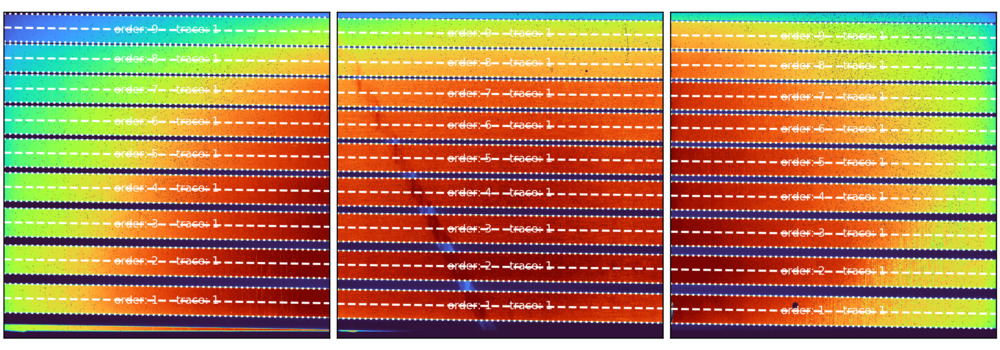
\includegraphics[width=0.9\linewidth]{tracetilt/Y1028_trace.jpg}

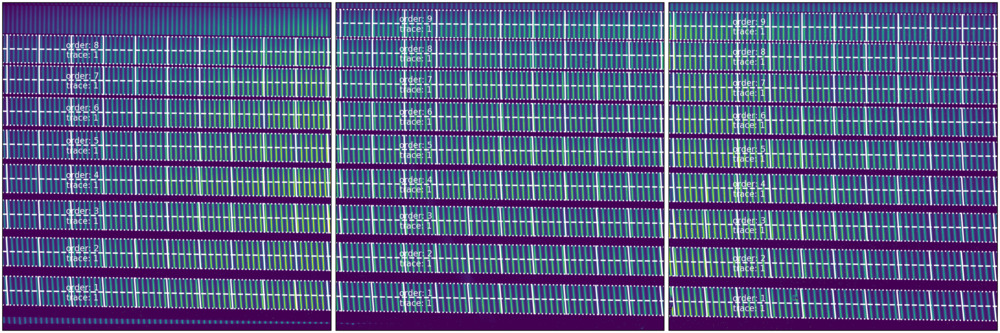
\includegraphics[width=0.9\linewidth]{tracetilt/Y1028_tilt.jpg}

\subsubsection*{Y1029}
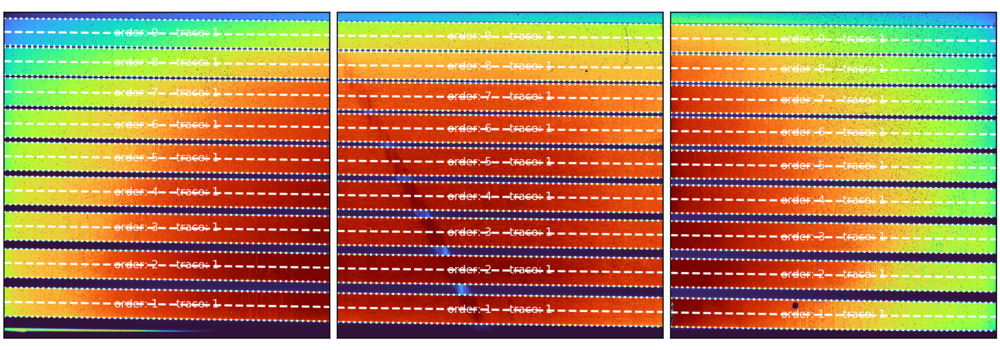
\includegraphics[width=0.9\linewidth]{tracetilt/Y1029_trace.jpg}

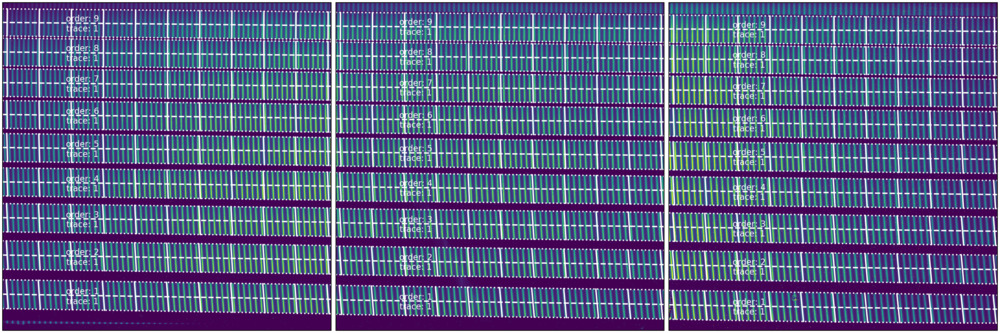
\includegraphics[width=0.9\linewidth]{tracetilt/Y1029_tilt.jpg}

\subsubsection*{J1226}
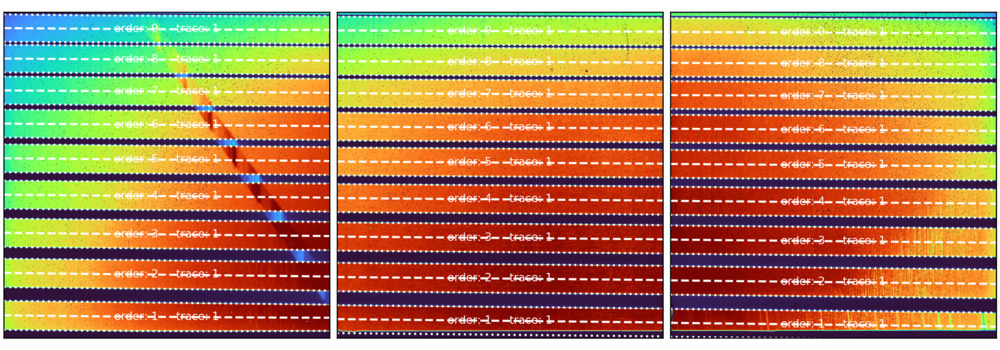
\includegraphics[width=0.9\linewidth]{tracetilt/J1226_trace.jpg}

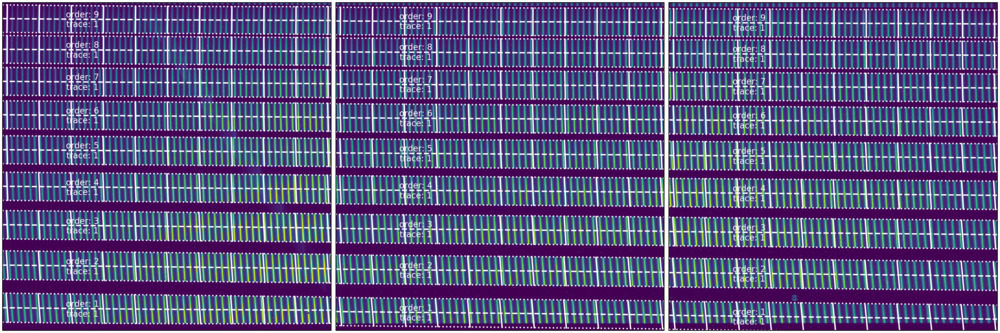
\includegraphics[width=0.9\linewidth]{tracetilt/J1226_tilt.jpg}

\subsubsection*{J1228}
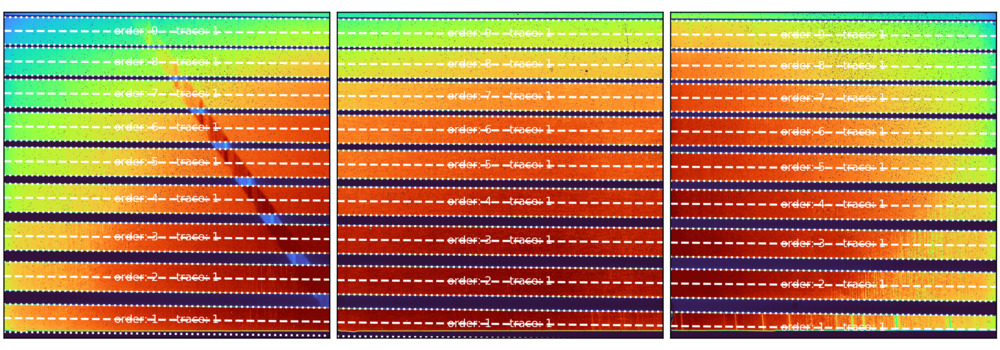
\includegraphics[width=0.9\linewidth]{tracetilt/J1228_trace.jpg}

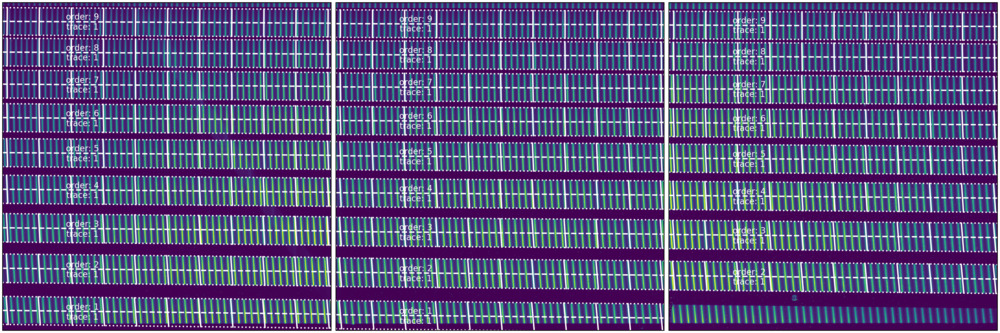
\includegraphics[width=0.9\linewidth]{tracetilt/J1228_tilt.jpg}

\subsubsection*{J1232}
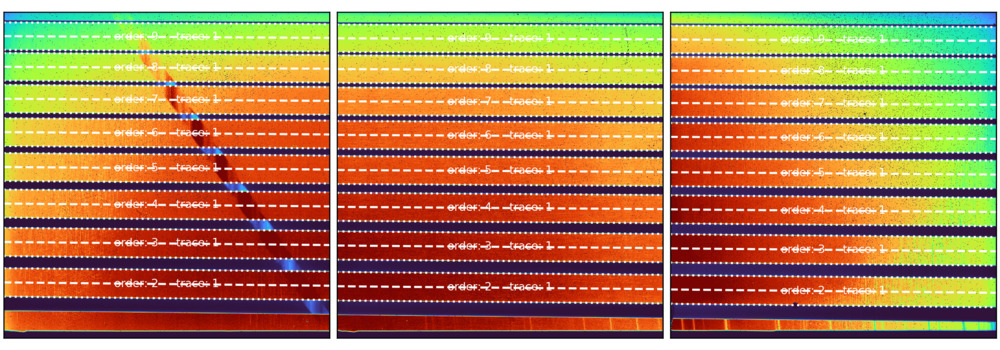
\includegraphics[width=0.9\linewidth]{tracetilt/J1232_trace.jpg}

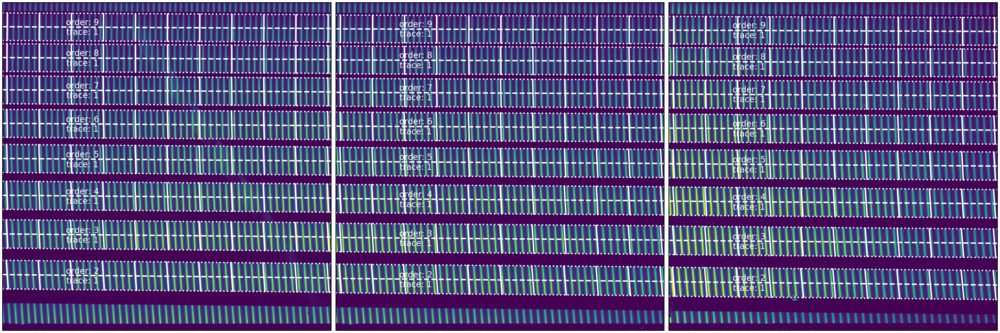
\includegraphics[width=0.9\linewidth]{tracetilt/J1232_tilt.jpg}

\subsubsection*{H1559}
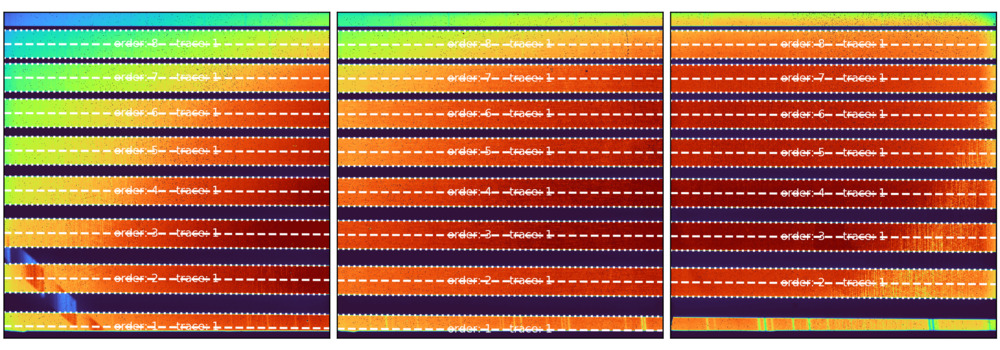
\includegraphics[width=0.9\linewidth]{tracetilt/H1559_trace.jpg}

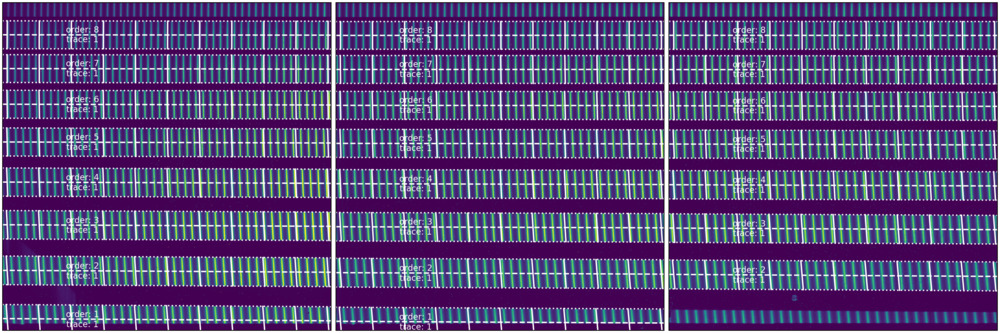
\includegraphics[width=0.9\linewidth]{tracetilt/H1559_tilt.jpg}

\subsubsection*{H1567}
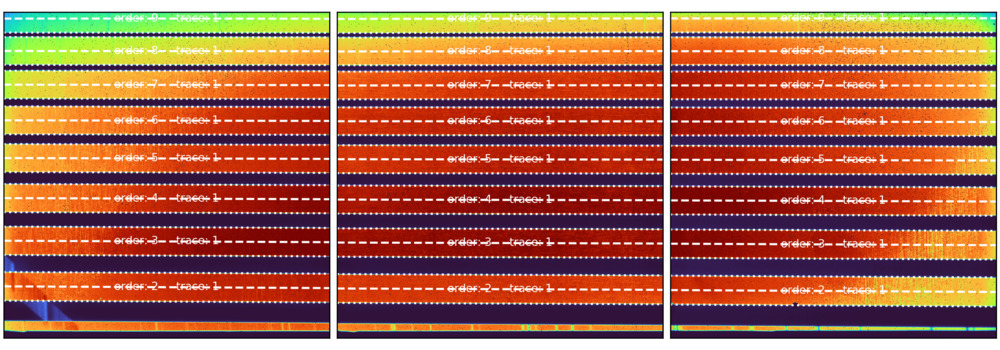
\includegraphics[width=0.9\linewidth]{tracetilt/H1567_trace.jpg}

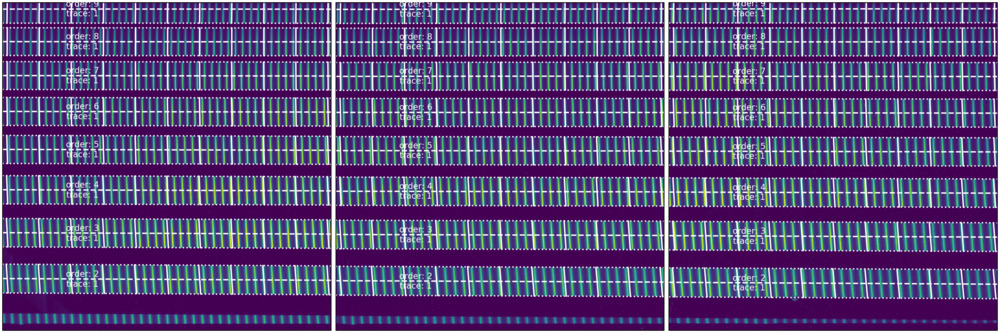
\includegraphics[width=0.9\linewidth]{tracetilt/H1567_tilt.jpg}

\subsubsection*{H1575}
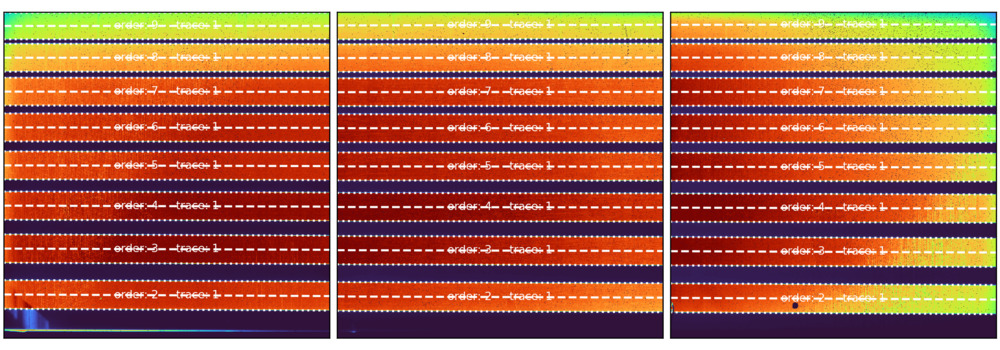
\includegraphics[width=0.9\linewidth]{tracetilt/H1575_trace.jpg}

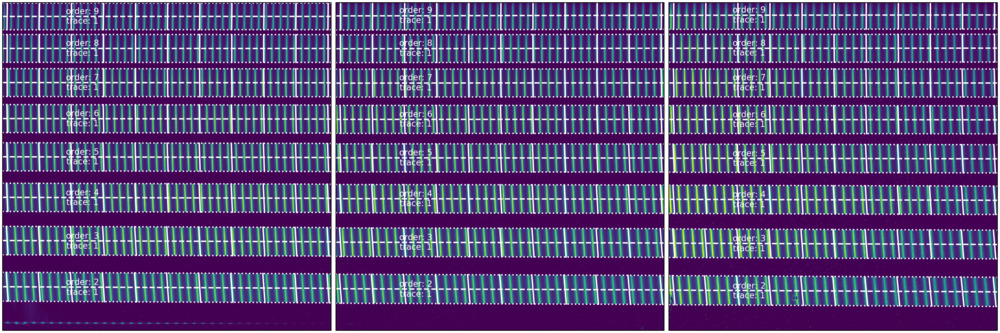
\includegraphics[width=0.9\linewidth]{tracetilt/H1575_tilt.jpg}

\subsubsection*{H1582}
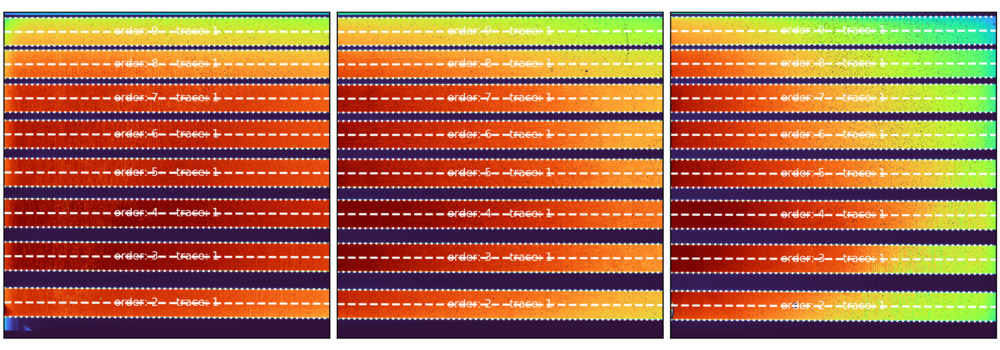
\includegraphics[width=0.9\linewidth]{tracetilt/H1582_trace.jpg}

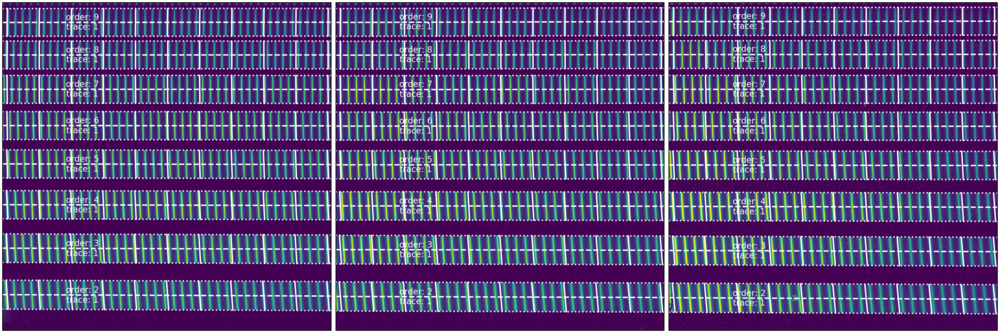
\includegraphics[width=0.9\linewidth]{tracetilt/H1582_tilt.jpg}

\subsubsection*{K2148}
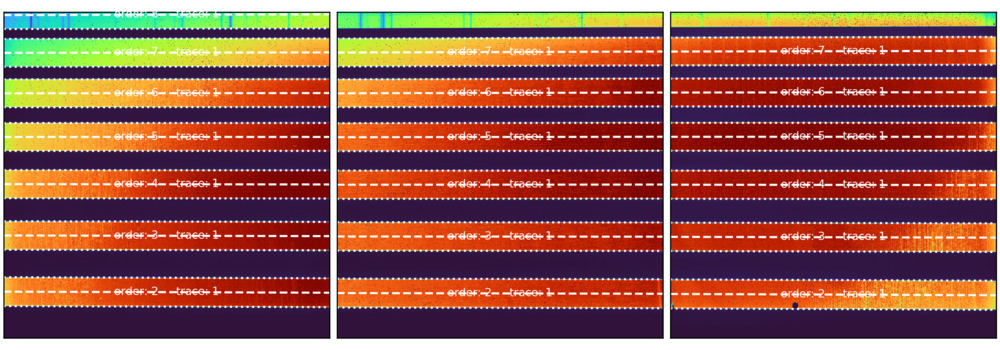
\includegraphics[width=0.9\linewidth]{tracetilt/K2148_trace.jpg}

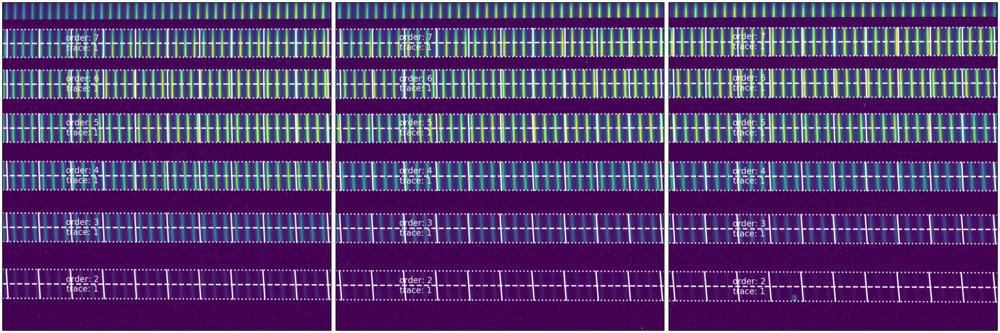
\includegraphics[width=0.9\linewidth]{tracetilt/K2148_tilt.jpg}

\subsubsection*{K2166}
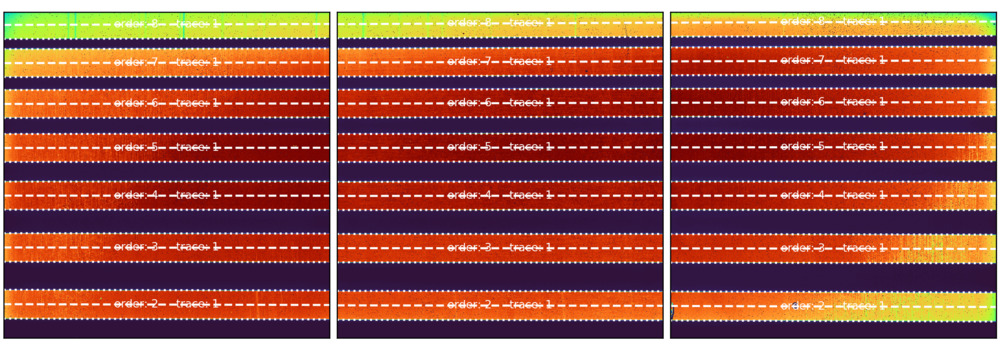
\includegraphics[width=0.9\linewidth]{tracetilt/K2166_trace.jpg}

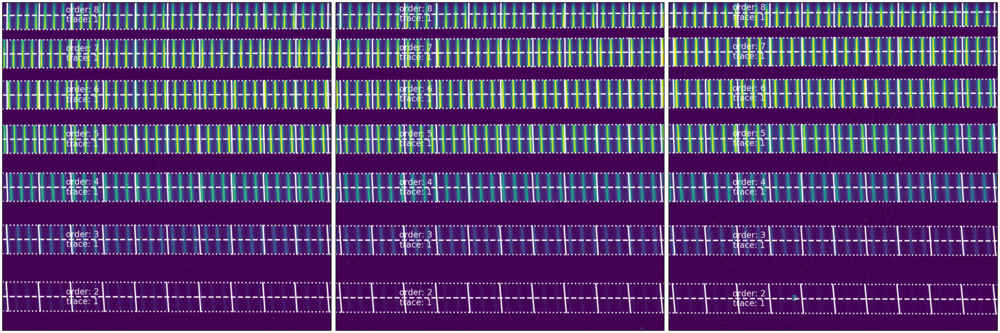
\includegraphics[width=0.9\linewidth]{tracetilt/K2166_tilt.jpg}

\subsubsection*{K2192}
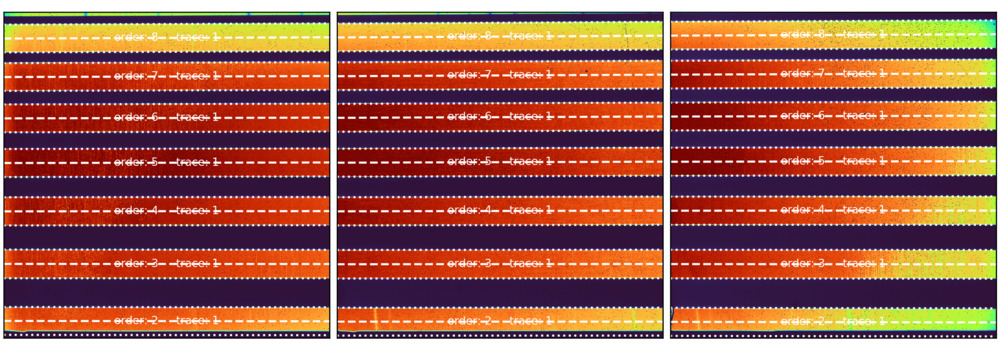
\includegraphics[width=0.9\linewidth]{tracetilt/K2192_trace.jpg}

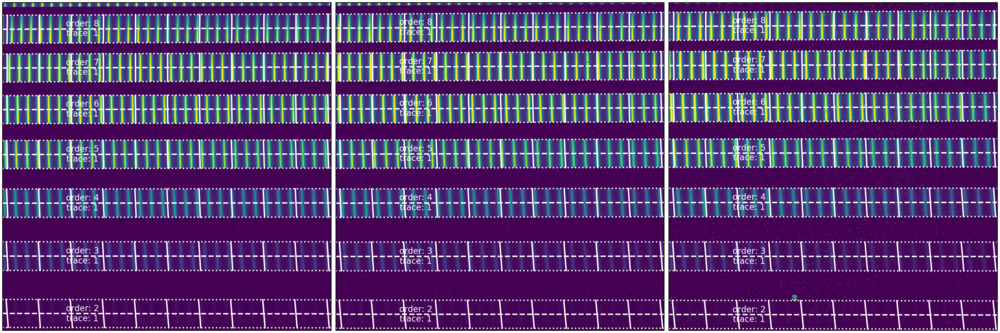
\includegraphics[width=0.9\linewidth]{tracetilt/K2192_tilt.jpg}

\subsubsection*{K2217}
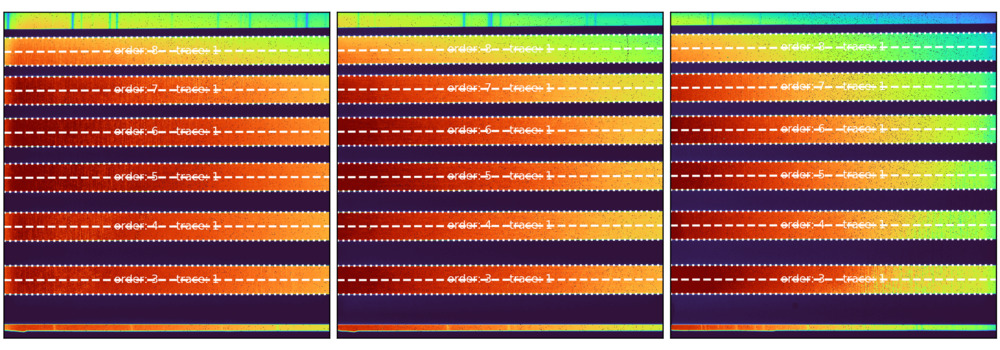
\includegraphics[width=0.9\linewidth]{tracetilt/K2217_trace.jpg}

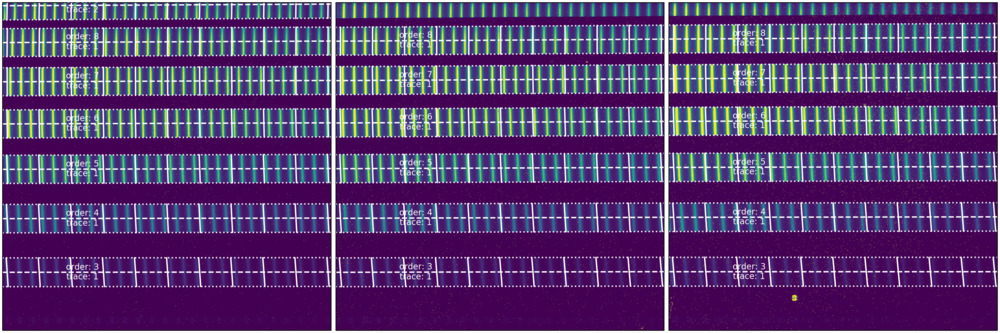
\includegraphics[width=0.9\linewidth]{tracetilt/K2217_tilt.jpg}

\subsubsection*{L3244}
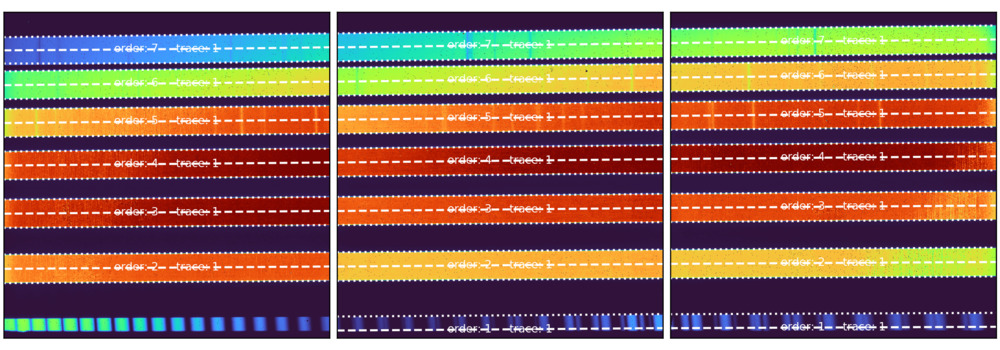
\includegraphics[width=0.9\linewidth]{tracetilt/L3244_trace.jpg}
\subsubsection*{L3262}
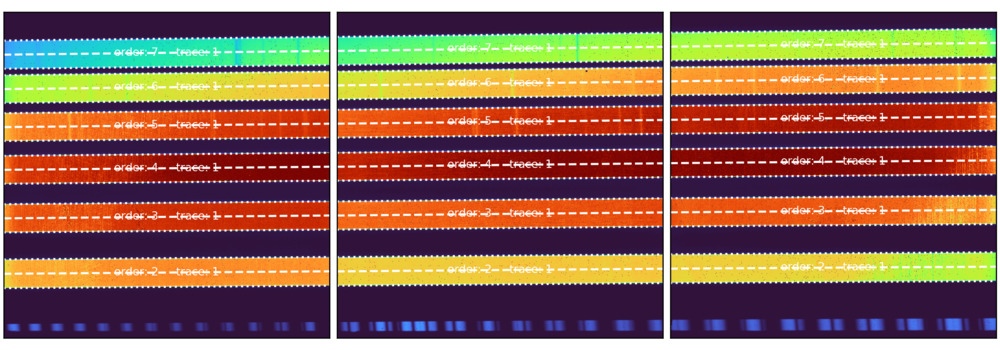
\includegraphics[width=0.9\linewidth]{tracetilt/L3262_trace.jpg}
\subsubsection*{L3302}
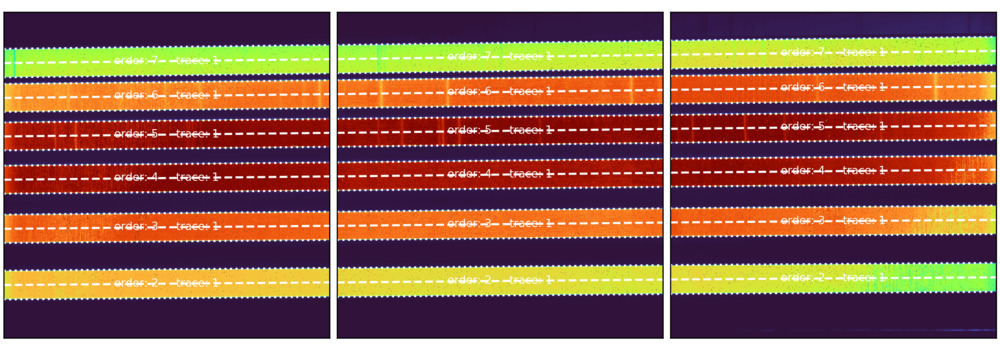
\includegraphics[width=0.9\linewidth]{tracetilt/L3302_trace.jpg}
\subsubsection*{L3340}
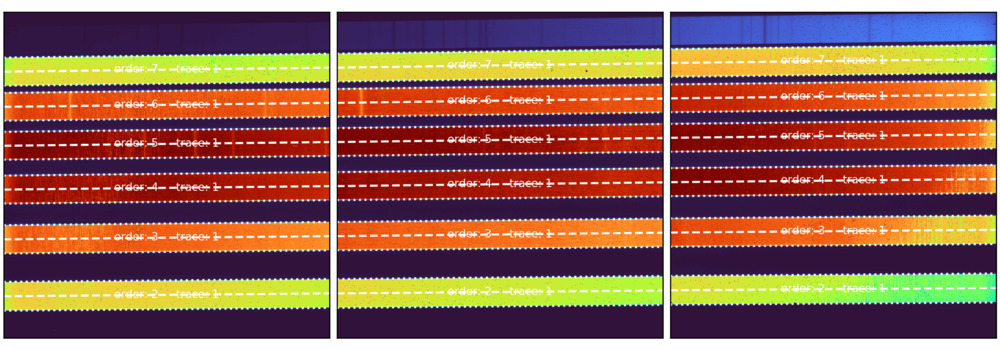
\includegraphics[width=0.9\linewidth]{tracetilt/L3340_trace.jpg}
\subsubsection*{L3377}
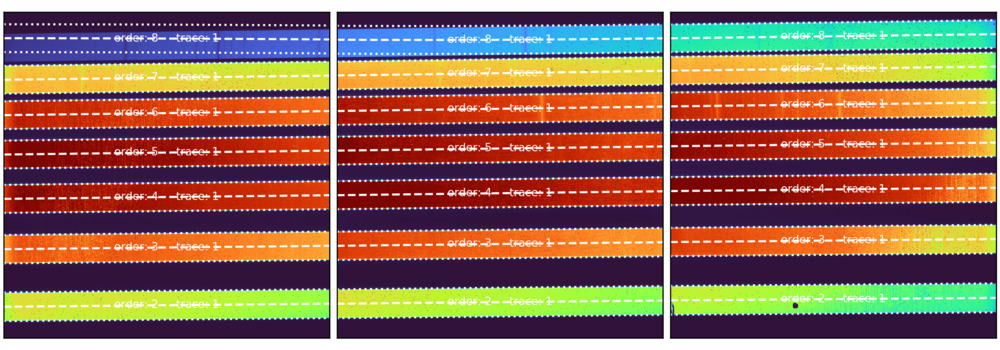
\includegraphics[width=0.9\linewidth]{tracetilt/L3377_trace.jpg}
\subsubsection*{L3412}
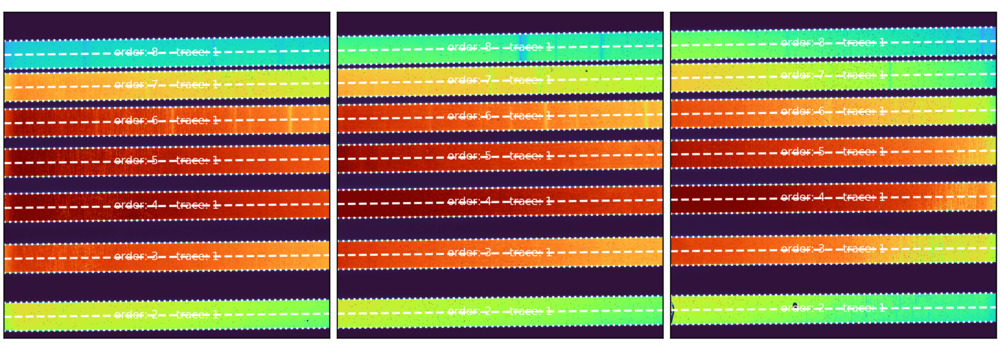
\includegraphics[width=0.9\linewidth]{tracetilt/L3412_trace.jpg}
\subsubsection*{L3426}
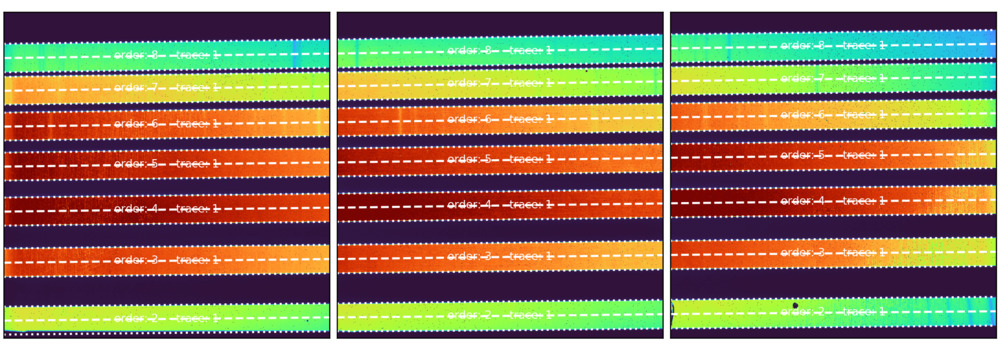
\includegraphics[width=0.9\linewidth]{tracetilt/L3426_trace.jpg}


\subsubsection*{M4187}
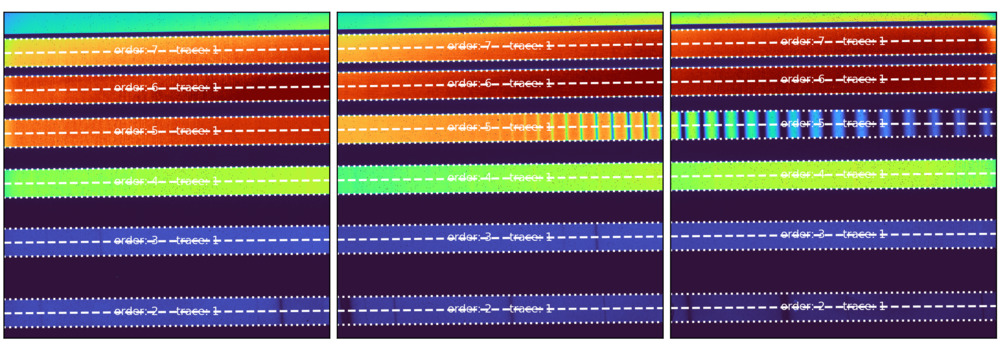
\includegraphics[width=0.9\linewidth]{tracetilt/M4187_trace.jpg}
\subsubsection*{M4211}
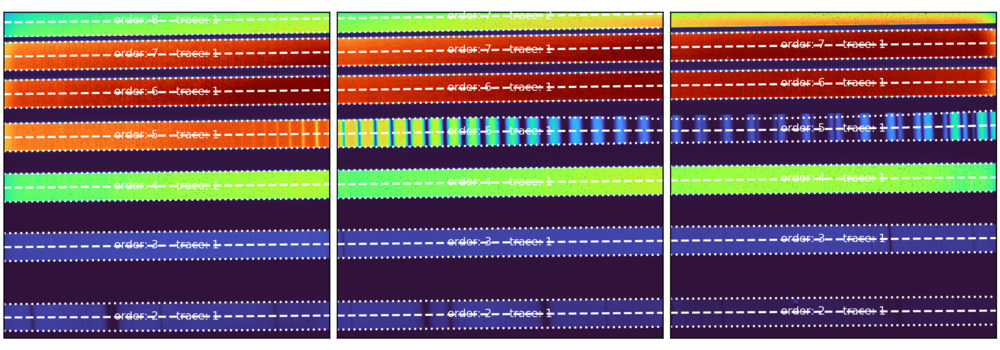
\includegraphics[width=0.9\linewidth]{tracetilt/M4211_trace.jpg}
\subsubsection*{M4266}
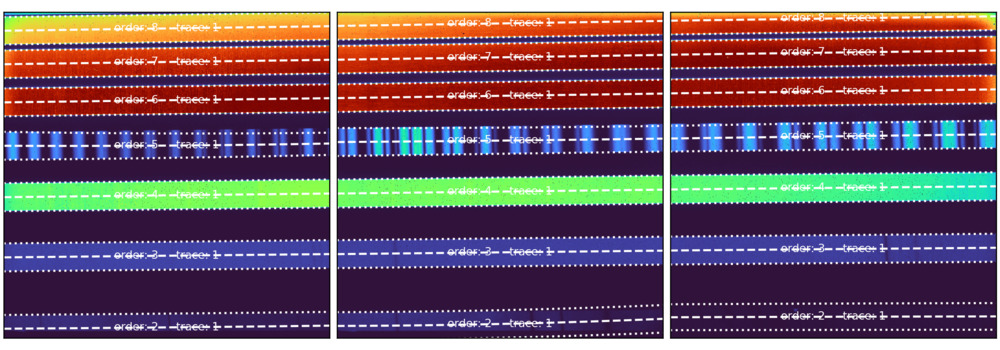
\includegraphics[width=0.9\linewidth]{tracetilt/M4266_trace.jpg}
\subsubsection*{M4318}
\includegraphics[width=0.9\linewidth]{tracetilt/M4318_trace.jpg}
\subsubsection*{M4368}
\includegraphics[width=0.9\linewidth]{tracetilt/M4368_trace.jpg}
\subsubsection*{M4416}
\includegraphics[width=0.9\linewidth]{tracetilt/M4416_trace.jpg}
\subsubsection*{M4461}
\includegraphics[width=0.9\linewidth]{tracetilt/M4461_trace.jpg}
\subsubsection*{M4504}
\includegraphics[width=0.9\linewidth]{tracetilt/M4504_trace.jpg}
\subsubsection*{M4519}
\includegraphics[width=0.9\linewidth]{tracetilt/M4519_trace.jpg}
\section{Processing reduced CRIRES data with MOLECFIT}
\label{sec:molecfit}


\subsection{Introduction}

Telluric lines - absorption from species in the Earth atmosphere - are strongly 
contaminating astronomical spectroscopic observation in the near-infrared, being
superimposed to the spectrum of the science target. The removal
of telluric lines from observations is therefore an important step in the reduction
and analysis of near-infrared spectra .

The removal of telluric lines is usually done either by observing a telluric standard star
close in time from the science target, or through the modelling of the telluric spectrum.
The latter method has the advantage of using no observing time. One tool of interest for 
ESO instruments which can model telluric spectrum and correct it in science spectra is {\tt MOLECFIT}
\footnote{{\tt MOLECFIT} can be downloaded at \url{https://www.eso.org/sci/software/pipelines/}} 
 \cite{smette-molecfit}.

The processing of CRIRES extracted spectra with {\tt MOLECFIT} is, at this point, neither
a part of the DRS nor supported by ESO. However, we provide here basic instructions and a custom script to convert
CRIRES reduced spectra into data which are ready to be processed with {\tt MOLECFIT}. This appendix
is not a tutorial, we assume that the user is familiar with {\tt MOLECFIT}. 

\subsection{Instructions}

We assume that the user has an extracted spectrum from the DRS, hereafter called input spectrum. It can be a spectrum:
\begin{itemize}
  \item acquired in staring or nodding mode
  \item  if from nodding: either from A or B position, or combined
\end{itemize}

The python script \verb!cr2res_drs2molecfit! will change the format of the input spectrum so that it can be processed with
{\tt MOLECFIT}. The primary extension of the output spectrum will be identical to the input spectrum. However,
every subsequent FITS extention will contain a spectral order projected on a single detector in table format with
threw columns: WAVE, SPEC, and ERR containing respectively the wavelength in microns, the spectrum, and the error spectrum.

The script \verb!cr2res_drs2molecfit! also creates a corresponding 
\begin{itemize}
  \item a \verb!WAVE_INCLUDE.fits! file, indicating the wavelength
region to be included in the fit. By default, all the spectrum is included, the user can modify the file if they wish.
  \item a  \verb!ATM_PARAMETERS_EXT.fits! file
\end{itemize}

Make sure to edit the configuration file for the \verb!molecfit_model! recipe with:
\begin{itemize}
 \item \verb!COLUMN_LAMBDA=WAVE!
 \item \verb!COLUMN_FLUX=SPEC!
 \item \verb!COLUMN_DFLUX=ERR!
\end{itemize}
so that {\tt MOLECFIT} can map the columns from the SCIENCE.fits file to wavelength, flux, and error arrays.

\section{UNE line selection}
\label{sec:uneselect}

\subsection*{Storing and using line selections}

\subsection*{Selecting lines}

\begin{figure}[ht]
    \begin{center}
\includegraphics[width=1.25\linewidth, angle=90]{linesel_examp.pdf}
\end{center}
\caption{An example of a UNe spectrum in setting J1228. }
\label{fig:linesel}
\end{figure}


avoid blends
matching relative strength.

goal is cross-correlation
different selection needed for line-fitting.

%\section{Scripts}
\label{sec:scripts}

There also exists a number of scripts, as listed below. Most are for visualization
purposes only. Nevertheless, they can serve as a starting point, for example for
how to open data products for further custom processing and analysis.

They do not perform necessary actions, and are not officially supported
-- please do not make support requests about them, or they might have to be
removed altogether in the future.

The scripts are not part of the RPM or MacPorts packages of the DRS, but are
included in the source-kit, downloadable from
\url{https://www.eso.org/sci/software/pipelines/}. Look for the file
\linebreak\verb!cr2re-X.X.X.tar.gz! within the source kit, and then the subdirectory
\verb!cr2re-X.X.X/tools/! therein.

Most likely you will have to look at the source code for how to use each script.
For the Python scripts, the only dependencies are \texttt{numpy},
\texttt{matplotlib} and \texttt{astropy.io.fits}. Shell scripts use bash-isms
and might or might not run in other shells.\footnote{Note that \texttt{/bin/sh}
is not linked to \texttt{bash} on many modern linux-systems.}

% in cr2rep/tools/
% ls *py | sed s/_/\\\\_/g | awk '//{printf "\\subsection{%s}\n",$1}'

\subsection{cr2res\_show\_raw.py}
Simply show raw (or calibrated) frames as a three-panel-plot. Cuts are chosen automatically unless given as first argument. Plots are saved as PNG-files with the same base name as the input.
\begin{shell}
    %prompt python3 show_raw.py 1,1000 somefile.fits another.fits
\end{shell}

\subsection{cr2res\_show\_trace.py}
Make a plot like Fig.~\ref{fig:flat_trace} by plotting the traces on top of any
frame, raw or otherwise.

\subsection{cr2res\_show\_trace\_curv.py}
Similar to previous, but also plots the slit-tilt in regular intervals. Examples
can be seen in App.~\ref{sec:extrafigs}.

\subsection{cr2res\_update\_wl.py}
Update the wavelength columns in extracted spectra from a TW table.

\subsection{cr2res\_show\_spec\_catal.py}
Plot extracted spectra against a catalog of lines. Also has some key-bindings
to select regions from cursor and re-fit a wavelength solution.

\subsection{cr2res\_plotresiduals.py}
Plot the residuals from line-diagnostics output.

\subsection{cr2res\_drs2molecfit.py}
Convert spectra to MolecFit-format, see Ch.~\ref{sec:molecfit}

\subsection{cr2res\_run\_setting.sh}
Reduce calibrations from a single setting from scratch, as in
Ch.~\ref{sec:calibscratch}. I has hardcoded paths, assumes data is organized in
a certain way and that plotting-scripts are in \verb!$PATH!, so this will not
run for users, but can serve as inspiration.

\subsection{cr2res\_makeSOFS.sh}
Companion script to the previous one, to set up directory structure and SOFs.

\subsection{cr2res\_measure\_lines.py}
\subsection{cr2res\_plot\_obs2d.py}
\subsection{cr2res\_plotfpet.py}
\subsection{cr2res\_plotsolution.py}
\subsection{cr2res\_select\_catalogue.py}
\subsection{cr2res\_show\_wavecal.py}
\subsection{cr2res\_wlen\_table.py}

\bibliography{cr2res-pipeline-manual}


\end{document}
